% !TEX encoding = UTF-8 Unicode

% ------------------------------------------------------------------------------------------------------
%	Formatvorlage für wissenschaftliche Arbeiten (Diplomarbeit, Bachelorarbeit, Masterarbeit)
% ------------------------------------------------------------------------------------------------------
%	ursprünglich erstellt von Stefan Macke, 24.04.2009
%	http://blog.stefan-macke.de
%
%	erweitert von Felix Rupp
%	http://www.felixrupp.com/
%
%	Version: 1.2
%	Datum: 21.05.2013


% Dokumentenkopf ---------------------------------------------------------------------------------------
%   Diese Vorlage basiert auf "scrreprt" aus dem koma-script.
% ------------------------------------------------------------------------------------------------------
\documentclass[
    12pt, % Schriftgröße
    DIV10, % Änderung der Größe des Satzspiegels (bedruckbarer Bereich einer Seite), nur in Verbindung mit koma-script verwendbar
    ngerman, % für Umlaute, Silbentrennung etc.
    a4paper, % Papierformat
    oneside, % einseitiges Dokument
    titlepage, % es wird eine Titelseite verwendet
    parskip=half, % Abstand zwischen Absätzen (halbe Zeile)
    headings=normal, % Größe der Überschriften verkleinern
    listof=totoc, % Verzeichnisse im Inhaltsverzeichnis aufführen
    bibliography=totoc, % Literaturverzeichnis im Inhaltsverzeichnis aufführen
    index=totoc, % Index im Inhaltsverzeichnis aufführen
    captions=tableheading, % Beschriftung von Tabellen unterhalb ausgeben
    final % Status des Dokuments (final/draft)
]{scrreprt}

% UTF8 und T1 Fontencoding -----------------------------------------------------------------------------
\usepackage[utf8]{inputenc}
\usepackage[T1]{fontenc}


% Meta-Informationen -----------------------------------------------------------------------------------
%   Informationen über das Dokument, wie z.B. Titel, Autor, Matrikelnr. etc
%   werden in der Datei Meta.tex definiert und können danach global
%   verwendet werden.
% ------------------------------------------------------------------------------------------------------
% !TEX encoding = UTF-8 Unicode
% !TEX root =  Bachelorarbeit.tex

% Meta-Informationen ------------------------------------------------------------------------------------
%   Definition von globalen Parametern, die im gesamten Dokument verwendet
%   werden können (z.B auf dem Deckblatt etc.).
%
%   ACHTUNG: Wenn die Texte Umlaute oder ein Esszet enthalten, muss der folgende
%            Befehl bereits an dieser Stelle aktiviert werden:
%            \usepackage[latin1]{inputenc}
% -------------------------------------------------------------------------------------------------------
\newcommand{\titel}{Implementierung einer interruptgesteuerten Benutzerschnittstelle}
\newcommand{\untertitel}{auf einem Low-Power-Mikrocontroller}
\newcommand{\untertitelDeckblatt}{auf einem Low-Power-Mikrocontroller}
\newcommand{\art}{Bachelor-Thesis}
\newcommand{\fachgebiet}{zur Erlangung des akademischen Grades\\ Bachelor of Science (B.\,Sc.) im Studienfach\xspace}
\newcommand{\autor}{Julian Rapp}
\newcommand{\keywords}{Bachelorarbeit, Julian Rapp}
\newcommand{\studienbereich}{Angewandte Informatik\xspace}
\newcommand{\matrikelnr}{304875}
\newcommand{\erstgutachter}{Prof. Dr. Irenäus Schoppa}
\newcommand{\zweitgutachter}{Prof. Dr. Heiko von Drachenfels}
\newcommand{\jahr}{2025}
\newcommand{\hochschule}{Hochschule für Technik, Wirtschaft und Gestaltung}
\newcommand{\ort}{Konstanz}
\newcommand{\logo}{Logo.png}
\newcommand{\creator}{TeXShop 3.16}



% benötigte Packages -----------------------------------------------------------------------------------
%   LaTeX-Packages, die benötigt werden, sind in die Datei Packages.tex
%   "ausgelagert", um diese Vorlage möglichst übersichtlich zu halten.
% ------------------------------------------------------------------------------------------------------
% !TEX encoding = UTF-8 Unicode
% !TEX root =  Bachelorarbeit.tex

% Anpassung des Seitenlayouts ---------------------------------------------------
%   siehe Seitenstil.tex
% -----------------------------------------------------------------------------------------
\usepackage[
    automark, % Kapitelangaben in Kopfzeile automatisch erstellen
    headsepline, % Trennlinie unter Kopfzeile
    ilines % Trennlinie linksbündig ausrichten
]{scrlayer-scrpage}


% Anpassung an Landessprache -------------------------------------------------
\usepackage[ngerman]{babel}


% Umlaute ------------------------------------------------------------------------------
%   Umlaute/Sonderzeichen wie äüöß direkt im Quelltext verwenden (CodePage).
%   Erlaubt automatische Trennung von Worten mit Umlauten.
%   Für Umlaute siehe Hauptdokument Zeile 35
% -----------------------------------------------------------------------------------------
\usepackage{textcomp} % Euro-Zeichen etc.


% Schrift --------------------------------------------------------------------------------
\usepackage{lmodern} % bessere Fonts
\usepackage{relsize} % Schriftgröße relativ festlegen


% Bessere Unterstreichungen ---------------------------------------------
\usepackage[normalem]{ulem}


% Grafiken -----------------------------------------------------------------------------
% Einbinden von JPG-Grafiken ermöglichen
\usepackage[dvips,final]{graphicx}
% hier liegen die Bilder des Dokuments
\graphicspath{{Bilder/}}


% Befehle aus AMSTeX für mathematische Symbole z.B. \boldsymbol \mathbb
\usepackage{amsmath,amsfonts}


% Eurozeichen benutzen ------------------------------------------------------------
\usepackage{eurosym}


% für Index-Ausgabe mit \printindex -----------------------------------------------
\usepackage{makeidx}


% Einfache Definition der Zeilenabstände und Seitenränder etc. ------------
\usepackage{setspace}
\usepackage{geometry}


% Symbolverzeichnis ------------------------------------------------------------------
%
%   Symbolverzeichnisse bequem erstellen. Beruht auf MakeIndex:
%     makeindex.exe %Name%.nlo -s nomencl.ist -o %Name%.nls
%   erzeugt dann das Verzeichnis unter WIndows. Dieser Befehl kann z.B. im TeXnicCenter
%   als Postprozessor eingetragen werden, damit er nicht ständig manuell
%   ausgeführt werden muss.
%
%   Unter Unix bitte einfach das mitgelieferte Shellskript "makemyindex" nutzen.
%
%   Die Definitionen werden im Fließtext mit den Befehlen:
%               - \Fachbegriff
%               - \FachbegriffSpezial
%               - \FachbegriffSpezialB
%    erzeugt oder separat in die Datei "Glossar.tex" eingetragen.
% -------------------------------------------------------------------------------------------
\usepackage[intoc]{nomencl}
\let\abbrev\nomenclature
\renewcommand{\nomname}{Abkürzungsverzeichnis und Glossar}
\setlength{\nomlabelwidth}{.25\hsize}
\renewcommand{\nomlabel}[1]{#1 \dotfill}
\setlength{\nomitemsep}{-\parsep}


% zum Umfließen von Bildern ---------------------------------------------------------
\usepackage[vflt]{floatflt}
\usepackage{subfigure}

% zum Einbinden von Programmcode -----------------------------------------------
\usepackage{listings}
\usepackage{xcolor} 
\definecolor{hellgelb}{rgb}{1,1,0.9}
\definecolor{colKeys}{rgb}{0.8,0,0.5}
\definecolor{colIdentifier}{rgb}{0.6,0,0.3}
\definecolor{colComments}{rgb}{0,0.5,0}
\definecolor{colString}{rgb}{0,0,1}

\lstset{
    float=htbp,
    basicstyle=\ttfamily\color{black}\small\smaller,
    identifierstyle=,%\color{colIdentifier},
    keywordstyle=\color{colKeys}\bfseries,
    stringstyle=\color{colString},
    commentstyle=\color{colComments},
    columns=flexible,
    tabsize=4,
    frame=single,
    extendedchars=true,
    showspaces=false,
    showstringspaces=false,
    numbers=left,
    numberstyle=\tiny,
    breaklines=true,
    backgroundcolor=\color{hellgelb},
    breakautoindent=true,
    escapeinside={(*}{*)},
    literate={Ö}{{\"O}}1 {Ä}{{\"A}}1 {Ü}{{\"U}}1 {ß}{{\ss}}2 {ü}{{\"u}}1 {ä}{{\"a}}1 {ö}{{\"o}}1 {µ}{\textmu}1
 }

% --------------------------------------------------------------------------------------------
% 
% Eigene Definitionen für Quelltext-Stile
%
% Define CSS:
\lstdefinelanguage{CSS}{
    morestring=[b]',
    morestring=[b]",
    comment=[l]{/*}{*/},
    sensitive=false,
    morekeywords={accelerator,adjust,after,align,attachment,azimuth,background,before,behavior,binding,border,bottom,bottomright,bottomleft,break,caption-side,char,clear,clip,color,colors,cue,cursor,collapse,decoration,direction,display,elevation,empty-cells,family,filter,float,flow,focus,font,grid,height,image,increment,indent,input,inside,ime-mode,include-source,justify,last,layer,left,letter,line,list,margin,marker,marks,max,min,mode,modify,moz,offsett,opacity,orphans,outline,overflow,overflow-X,overflow-Y,overhang,position,position-x,position-y,padding,page,pause,pitch,play-during,position,quotes,radius,range,repeat,replace,reset,richness,right,ruby,set-link-source,select,shadow,size,spacing,speak,speak-header,speak-numeral,speak-punctuation,speech-rate,stress,stretch,style,table-layout,text,transform,text-autospace,text-kashida-space,top,topleft,topright,type,underline,unicode-bidi,use-link-source,user,variant,vertical,visibility,voice-family,volume,white-space,weight,widows,width,word,wrap,word-wrap,writing-mode,z-index,zoom}
}


% Define JavaScript:
\lstdefinelanguage{JavaScript}{
  keywords={typeof, new, true, false, catch, function, return, null, catch, switch, var, if, in, while, do, else, case, break},
  keywordstyle=\color{colKeys}\bfseries,
  ndkeywords={class, export, boolean, throw, implements, import, this},
  ndkeywordstyle=\color{darkgray}\bfseries,
  sensitive=false,
  comment=[l]{//},
  morecomment=[s]{/*}{*/},
  morestring=[b]',
  morestring=[b]"
}

% Define TypoScript:
\lstdefinelanguage{TypoScript}{
  keywords=[1]{PAGE, HTML, TEXT, COA, COA\_INT, FILE, IMAGE, IMG\_RESOURCE, CLEARGIF, CONTENT, RECORDS, HMENU, CTABLE, OTABLE, COLUMNS, HRULER, IMGTEXT, CASE, LOAD\_REGISTER, RESTORE\_REGISTER, FORM, SEARCHRESULT, USER, USER\_INT, TEMPLATE, FLUIDTEMPLATE, MULTIMEDIA, SVG, EDITPANEL, GIFBUILDER, GMENU, TMENU, TMENUITEM, IMGMENU, IMGMENUITEM, JSMENU, JSMENUITEM, BOX},
  keywordstyle=[1]{\color{blue}\bfseries},
  keywords=[2]{plugin, view, page, file, text, config},
  keywordstyle=[2]{\color{blue}\bfseries},
  keywords=[3]{EXT},
  keywordstyle=[3]{\color{blue}\bfseries},
  sensitive=true,
  comment=[l]{\#\ }
}

% PHP5 dialect 
\lstdefinelanguage[5]{PHP}[]{PHP} {
  morekeywords={
  %--- class and exceptions keywords 
  class,static,private,public,abstract,interface,const,function,require_once,final,new,extends,implements,
  %--- additional array functions 
  array_combine,array_diff_uassoc,array_udiff,array_udiff_assoc,% 
  array_udiff_uassoc,array_walk_recursive,array_uintersect_assoc,% 
  array_usintersect_uassoc,array_uintersect,% 
  %--- string functions 
  str_split, strpbrk,substr_compare 
  %--- Date and time functions 
  idate,date_sunset,date_sunrise,time_nanosleep,
  %--- return
  return
  } 
} 


% Fluid dialect 
\lstdefinelanguage[Fluid]{HTML}[]{HTML} {
  morekeywords={if, for, each, as, condition, controller, arguments, image, link, action, class} 
} 


% URL verlinken, lange URLs umbrechen etc. -------------------------------------
\usepackage{url}


% natbib einbinden -----------------------------------------------------------------------
%\usepackage[numbers]{natbib}

% csquotes einbinden ---------------------------------------------------------------------
\usepackage{csquotes}

% biblatex einbinden ---------------------------------------------------------------------
\usepackage[
	style=numeric,
	backend=biber,
	citestyle=numeric,
	sorting=ynt
]{biblatex}

\usepackage{ifthen}

% PDF-Optionen -------------------------------------------------------------------------
\usepackage[
    bookmarks,
    bookmarksopen=true,
    colorlinks=true,
% diese Farbdefinitionen zeichnen Links im PDF farblich aus
    linkcolor=red, % einfache interne Verknüpfungen
    anchorcolor=black,% Ankertext
    citecolor=blue, % Verweise auf Literaturverzeichniseinträge im Text
    filecolor=magenta, % Verknüpfungen, die lokale Dateien öffnen
    menucolor=red, % Acrobat-Menüpunkte
    urlcolor=cyan, 
%
% diese Farbdefinitionen sollten für den Druck verwendet werden (alles schwarz):
%
    %linkcolor=black, % einfache interne Verknüpfungen
    %anchorcolor=black, % Ankertext
    %citecolor=black, % Verweise auf Literaturverzeichniseinträge im Text
    %filecolor=black, % Verknüpfungen, die lokale Dateien öffnen
    %menucolor=black, % Acrobat-Menüpunkte
    %urlcolor=black, 
%
    %backref,
    plainpages=false, % zur korrekten Erstellung der Bookmarks
    pdfpagelabels, % zur korrekten Erstellung der Bookmarks
    hypertexnames=false, % zur korrekten Erstellung der Bookmarks
    linktocpage % Seitenzahlen anstatt Text im Inhaltsverzeichnis verlinken
]{hyperref}
% Befehle, die Umlaute ausgeben, führen zu Fehlern, wenn sie hyperref als Optionen übergeben werden
\hypersetup{
    pdftitle={\titel \untertitel},
    pdfauthor={\autor},
    pdfcreator={\creator},
    pdfsubject={\titel \untertitel},
    pdfkeywords={\keywords},
}

% Paket zum sauberen Einbauen von externen PDF-Dateien -----------------
\usepackage[final]{pdfpages}


% fortlaufendes Durchnummerieren der Fußnoten -------------------------------
\usepackage{chngcntr}


% schönere Tabellen --------------------------------------------------------------------
\usepackage{tabularx}
\usepackage{multirow}


% für lange Tabellen ---------------------------------------------------------------------
\usepackage{longtable}
\usepackage{ltxtable}
\usepackage{filecontents}
\usepackage{array}
\usepackage{ragged2e}
\usepackage{lscape}


% Rotation von Elementen -------------------------------------------------------
\usepackage{rotating}


% Formatierung von Listen ändern --------------------------------------------------
\usepackage{paralist}
\usepackage{enumitem}


% bei der Definition eigener Befehle benötigt -------------------------------------
\usepackage{ifthen}
\usepackage{forloop}


% definiert u.a. die Befehle \todo und \listoftodos --------------------------------
\usepackage{todonotes}


% sorgt dafür, dass Leerzeichen hinter parameterlosen Makros nicht als Makroendezeichen interpretiert werden
\usepackage{xspace}



% Erstellung eines Index und Abkürzungsverzeichnisses/Glossars aktivieren ------------------------------
\makeindex{}
\makenomenclature{}


% Kopf- und Fußzeilen, Seitenränder etc. ---------------------------------------------------------------
% !TEX encoding = UTF-8 Unicode
% !TEX root =  Bachelorarbeit.tex

% Zeilenabstand 1,5 Zeilen ---------------------------------------------------------------------
\onehalfspacing{}


% Seitenränder ------------------------------------------------------------------------------------
\setlength{\topskip}{\ht\strutbox} % behebt Warnung von geometry
\geometry{paper=a4paper,left=30mm,right=30mm,top=30mm}


% Kopf- und Fußzeilen --------------------------------------------------------------------------
\pagestyle{scrheadings}

% Kopf- und Fußzeile auch auf Kapitelanfangsseiten
\renewcommand*{\chapterpagestyle}{scrheadings} 

% Schriftform der Kopfzeile
\renewcommand{\headfont}{\normalfont}


% Kopfzeile für einseitiges Dokument:
\ihead{%\small{\textsc{\titel}	\\
	%\untertitel
	%\\[2ex]
	\textit{\headmark}%}
}
\chead{}
\rohead{\includegraphics[scale=0.3]{\logo}}
\setlength{\headheight}{21mm} % Höhe der Kopfzeile
% Kopfzeile über den Text hinaus verbreitern
\setheadwidth[0pt]{textwithmarginpar} 
\setheadsepline[text]{0.4pt} % Trennlinie unter Kopfzeile


%% Kopfzeile für Zweiseitiges Dokument:
%\ihead{\textit{\leftmark}}
%\chead{}
%\ohead{}
%\lehead{\includegraphics[scale=0.25]{\logo}}
%\rohead{\includegraphics[scale=0.25]{\logo}}
%\setheadsepline[text]{0.4pt} % Trennlinie unter Kopfzeile


% Fußzeile
%\ifoot{\copyright\ \autor}
\cfoot{}
\ofoot{\pagemark \\[4ex]}


% sonstige typographische Einstellungen ---------------------------------------------------
% erzeugt ein wenig mehr Platz hinter einem Punkt
\frenchspacing{}

% Schusterjungen und Hurenkinder vermeiden
\clubpenalty = 10000
\widowpenalty = 10000 
\displaywidowpenalty = 10000

% Quellcode-Ausgabe formatieren
\lstset{numbers=left, numberstyle=\tiny, numbersep=5pt, breaklines=true}
\lstset{emph={square}, emphstyle=\color{red}, emph={[2]root,base}, emphstyle={[2]\color{blue}}}

% Fußnoten fortlaufend durchnummerieren
\counterwithout{footnote}{chapter}




% eigene Definitionen für Silbentrennung ---------------------------------------------------------------
% !TEX encoding = UTF-8 Unicode
% !TEX root =  Bachelorarbeit.tex

% Trennvorschläge im Text werden mit \" angegeben
% untrennbare Wörter und Ausnahmen von der normalen Trennung können in dieser
% Datei mittels \hyphenation definiert werden

\hyphenation{End-an-wen-der}
\hyphenation{sym-bo-li-siert}
\hyphenation{for-ma-te}
\hyphenation{Ma-nage-ment}
\hyphenation{An-for-de-rungs-be-schrei-bung}
\hyphenation{Cor-po-rate}
\hyphenation{De-sign}
\hyphenation{Pro-gram-mier-schnitt-stel-le}
\hyphenation{in-ter-rupt-ge-steu-er-ten}
\hyphenation{Be-nut-zer-schnitt-stel-le}
\hyphenation{in-ter-rupt-ge-st-e-u-er-ten}
\hyphenation{Low-Power-Microcontroller}
\hyphenation{Steu-er-ein-heit}
\hyphenation{Echt-zeit-ver-hal-ten}
\hyphenation{Cap-ture/Com-pa-re-Re-gis-tern}
\hyphenation{Pro-gramm-un-ter-bre-chun-gen}
\hyphenation{un-er-l\"as-slich}
\hyphenation{Hoch-ge-sch-win-dig-keits-kom-mu-ni-ka-ti-on}
\hyphenation{Kom-mu-ni-ka-tions-schnit-ts-tel-le}
\hyphenation{Ter-mi-nie-rungs-zei-chen}
\hyphenation{null-ter-mi-nie-rungs-zei-chen}
\hyphenation{Ein-ga-be}


% eigene LaTeX-Befehle ---------------------------------------------------------------------------------
% !TEX encoding = UTF-8 Unicode
% !TEX root =  Bachelorarbeit.tex
% Eigene Befehle und typographische Auszeichnungen für diese


% einfaches Wechseln der Schrift, z.B.: \changefont{cmss}{sbc}{n} ---------------------------------------
\newcommand{\changefont}[3]{\fontfamily{#1} \fontseries{#2} \fontshape{#3} \selectfont}


% Abkürzungen mit korrektem Leerraum --------------------------------------------------------------------
\newcommand{\ua}{\mbox{u.\,a.\ }}
\newcommand{\zB}{\mbox{z.\,B.\ }}
\newcommand{\dahe}{\mbox{d.\,h.\ }}
\newcommand{\Vgl}{Vgl.\ }
\newcommand{\bzw}{bzw.\ }
\newcommand{\evtl}{evtl.\ }
\newcommand{\ggf}{ggf.\ }

\newcommand{\Abbildung}[1]{Abbildung~\ref{fig:#1}}
\newcommand{\Tabelle}[1]{Tabelle~\ref{tab:#1}}

\newcommand{\bs}{$\backslash$}


% erzeugt ein Listenelement mit fetter Überschrift ------------------------------------------------------
\newcommand{\itemd}[2]{\item{\textbf{#1}}\\{#2}}


% einige Befehle zum Zitieren ---------------------------------------------------------------------------
\newcommand{\Zitat}[2][\empty]{%
	\ifthenelse{\equal{#1}{\empty}}%
	{\cite{#2}}%
	{\cite[#1]{#2}}%
}
%\newcommand{\Zitat}[2][\empty]{\ifthenelse{\equal{#1}{\empty}}{\citep{#2}}{\citep[#1]{#2}}}
\newcommand{\ZitatSpezialA}[3]{\citep[#1][#2]{#3}}
\newcommand{\ZitatSpezialB}[2]{\citep[#1][]{#2}}


% zum Ausgeben von Autoren
\newcommand{\AutorName}[1]{\textsc{#1}}
\newcommand{\Autor}[1]{\AutorName{\citeauthor{#1}}}


% verschiedene Befehle um Wörter semantisch auszuzeichnen -----------------------------------------------
\newcommand{\NeuerBegriff}[1]{\textbf{#1}}

\newcommand{\Abkuerzung}[2]{\textit{#2}\nomenclature{#2}{#1}}

\newcommand{\Fachbegriff}[2][\empty]{\ifthenelse{\equal{#1}{\empty}}{\textit{#2}\xspace}{\textit{#2}\xspace\footnote{#1}\nomenclature{#2}{#1}}}

\newcommand{\FachbegriffSpezialA}[4]{\textit{#4}\footnote{#3}\label{fn:#1}\nomenclature{#4}{#2. Siehe auch Fu{\ss}zeile auf Seite~\pageref{fn:#1}.}}

\newcommand{\FachbegriffSpezialB}[5]{\textit{#5}\footnote{#3}\label{fn:#1}\nomenclature{#4}{#2. Siehe auch Fu{\ss}zeile auf Seite~\pageref{fn:#1}.}}


% Beträge mit Währung -----------------------------------------------------------------------------------
\newcommand{\Betrag}[2][general]{#2\,\ifthenelse{\equal{#1}{dollar}}{\$}{}\ifthenelse{\equal{#1}{euro}}{€}{}\ifthenelse{\equal{#1}{yen}}{¥}{}\ifthenelse{\equal{#1}{cent}}{¢}{}\ifthenelse{\equal{#1}{pound}}{£}{}\ifthenelse{\equal{#1}{peso}}{₱}{}\ifthenelse{\equal{#1}{baht}}{฿}{}\ifthenelse{\equal{#1}{franc}}{₣}{}\ifthenelse{\equal{#1}{lira}}{₤}{}\ifthenelse{\equal{#1}{drachma}}{₯}{}\ifthenelse{\equal{#1}{pfennig}}{₰}{}\ifthenelse{\equal{#1}{general}}{¤}{}}


% Sonstiges ---------------------------------------------------------------------------------------------
\newcommand{\Eingabe}[1]{\texttt{#1}}
\newcommand{\Code}[1]{\texttt{#1}}	% Monotype oder Type Writer
\newcommand{\Datei}[1]{\texttt{#1}}

\newcommand{\Datentyp}[1]{\textsf{#1}}
\newcommand{\XMLElement}[1]{\textsf{#1}}
\newcommand{\Webservice}[1]{\textsf{#1}}


% Beschriftung von Tabellen und Bildern ändern ----------------------------------------------------------
\addto\captionsngerman{
	\renewcommand{\figurename}{Abb.}
	\renewcommand{\tablename}{Tab.}
}

% Hinweis auf Unterstütztes schreiben durch AI
\newcommand{\AI}{\footnote{Die sprachliche \"Uberarbeitung dieses Kapitels erfolgte unter Zuhilfenahme von KI-Sprachmodellen. Inhaltliche Aussagen und Schlussfolgerungen stammen ausschlie{\ss}lich vom Autor.}}


% Spaltendefinition rechtsbündig mit definierter Breite -------------------------------------------------
\newcolumntype{w}[1]{>{\raggedleft\hspace{0pt}}p{#1}}


% Linksbündige Tabellenspalten mit tabularx -------------------------------------------------------------
\newcolumntype{y}[1]{>{\RaggedRight\arraybackslash\hsize=#1\hsize}X}



% Das eigentliche Dokument -----------------------------------------------------------------------------
%   Der eigentliche Inhalt des Dokuments beginnt hier. Die einzelnen Seiten
%   und Kapitel werden in eigene Dateien ausgelagert und hier nur inkludiert.
% ------------------------------------------------------------------------------------------------------
\begin{document}


% auch subsubsections nummerieren ----------------------------------------------------------------------
\setcounter{secnumdepth}{3}
% Nummerierungsebenen im Inhaltsverzeichnis
\setcounter{tocdepth}{2}


% Deckblatt und Abstract ohne Seitenzahl ---------------------------------------------------------------
\ofoot{}
% !TEX encoding = UTF-8 Unicode
% !TEX root =  Bachelorarbeit.tex

\thispagestyle{plain}
\begin{titlepage}

\changefont{cmss}{bx}{n}

\begin{flushleft}

\LARGE{\textbf{\titel}}\\[1.5ex]
\Large{\textbf{\untertitelDeckblatt}}\\[6ex]
\Large{\textbf{\art}}\\[1.5ex]

\changefont{cmss}{m}{n}
\large{\fachgebiet \studienbereich}\\[12ex]



\includegraphics[width=0.7\textwidth]{Logo.png}\\[12ex]

\normalsize{}
\begin{tabular}{ll}
vorgelegt von:  & \quad \autor\\[1.2ex]
Matrikelnummer: & \quad \matrikelnr\\[1ex]
Erstgutachter:  & \quad \erstgutachter\\[1ex]
Zweitgutachter: & \quad \zweitgutachter\\[1ex]
eingereicht in: & \quad \ort, am 30.\,Juni\,2025
\end{tabular}

\end{flushleft}


% Die folgenden Kommentare entfernen um einen Sperrvermerk auf der 2. Seite zu erzeugen
%\singlespacing

%\newpage

%\thispagestyle{empty}

%\changefont{cmr}{m}{n}

%\small
%\noindent Die nachfolgende \art\ \textbf{enth\"alt vertrauliche Daten der Musterfabrik GmbH \& Co. Betriebs KG}. Ver\"offentlichungen oder Vervielf\"altigungen -- auch auszugsweise -- sind ohne ausdr\"uckliche Genehmigung der Musterfabrik GmbH \& Co. Betriebs KG nicht gestattet. Die \art\ ist nur den Erst- und Zweitgutachtern und dem Prüfungsausschuss zug\"anglich zu machen.\\[5ex]

\end{titlepage}

% !TEX encoding = UTF-8 Unicode
% !TEX root =  ../Bachelorarbeit.tex
\chapter*{Zitat}
\label{cha:Zitat}

\thispagestyle{empty}

\begin{center}
\begin{minipage}{14cm}
\begin{verse}
\textit{So I listen to the radio and all the songs we used to know \\
So I listen to the radio remember where we used to go}

(The Corrs -- Radio)
\end{verse}
%\hfill \textsf 
\end{minipage}
\end{center}

% !TEX encoding = UTF-8 Unicode
% !TEX root =  ../Bachelorarbeit.tex

\chapter*{Abstract}
\label{cha:Abstract}

\thispagestyle{empty}


Die vorliegende wissenschaftliche Arbeit behandelt die Planung und Entwicklung einer interruptgesteuerten Benutzerschnittstelle zur Überwachung und Manipulation von Registern und Speicherzellen. Die Entwicklung soll auf Basis eines Low-Power-Microcontrollers der MSP430 Familie von Texas Instruments erfolgen.
\\
Es erfolgt eine umfangreiche Planungs-/ und Entwicklungsphase, die in Anlehnung an den Rational Unified Process dokumentiert wird. Auf Basis dieser Planung wird die Software dann als austauschbares Modul implementiert. Der Vorgang der praktischen Umsetzung wird schriftlich dokumentiert. Zum Abschluss der Arbeit wird die Erweiterung im Live-Betrieb des Praktikums von Microprozessorsysteme zum Einsatz kommen.
\ofoot{\pagemark \\[4ex]}


% Seitennummerierung -----------------------------------------------------------------------------------
%   Vor dem Hauptteil werden die Seiten in großen römischen Ziffern 
%   nummeriert.
% ------------------------------------------------------------------------------------------------------
\pagenumbering{Roman}
\phantomsection{} % Sorgt für korrekte Aufnahme des Inhaltsverzeichnisses in das Inhaltsverzeichnis
\addcontentsline{toc}{chapter}{Inhaltsverzeichnis}
\tableofcontents{}


% Abkürzungsverzeichnis --------------------------------------------------------------------------------
% !TEX encoding = UTF-8 Unicode
% !TEX root =  ../Bachelorarbeit.tex

%\nomenclature{TEST}{Dummy}
% für korrekte Überschrift in der Kopfzeile
\clearpage\markboth{\nomname}{\nomname} 
\printnomenclature{}
\label{sec:Glossar}


% arabische Seitenzahlen im Hauptteil ------------------------------------------------------------------
\clearpage{}
\pagenumbering{arabic}


% die Inhaltskapitel werden in "Inhalt.tex" inkludiert -------------------------------------------------
% !TEX encoding = UTF-8 Unicode
% !TEX root =  Bachelorarbeit.tex

% Hier können die einzelnen Kapitel inkludiert werden. Sie müssen in den 
% entsprechenden .TEX-Dateien vorliegen. Die Dateinamen können natürlich 
% angepasst werden.

% !TEX encoding = UTF-8 Unicode
% !TEX root =  ../Bachelorarbeit.tex

\chapter{Einleitung}
\label{cha:Einleitung}


\section{Das Ziel dieser Arbeit}
\label{sec:ZielDerArbeit}

Diese Bachelor-Thesis befasst sich mit der Entwicklung einer \Fachbegriff{Ein Mechanismus zur ereignisorientierten Unterbrechung des normalen Programmablaufs}{interruptgesteuerten}[interruptgesteuert] Benutzerschnittstelle auf einem \Fachbegriff{Ein Mikrocontroller, der f\"ur energieeffiziente Anwendungen optimiert ist. Typischerweise eingesetzt in batteriebetriebenen Embedded-Systemen}{Low-Power-Mikrocontroller}, zur \"Uberwachung und Manipulation von \Fachbegriff{Speicherzellen, die fl\"uchtig sind und ihre Inhalte beim Ausschalten verlieren}{Registern}[Register] und Speicherzellen in \Abkuerzung{Random Access Memory}{RAM} und \Abkuerzung{Ferroelectric Random Access Memory}{FRAM}.

Im Zuge des Arbeitsauftrags wird ein unabh\"angiges \Fachbegriff{Eine funktionale Einheit innerhalb eines gr\"o{\ss}eren Systems, die separat entwickelt und gewartet werden kann}{Modul} entwickelt, welches nach Wunsch aktiviert oder deaktiviert wird.


\section{Die Umgebung, in der die Arbeit entstand}
\label{sec:EntstehungsUmgebungArbeit}

Die Entwicklung der Software geschah in Absprache mit Herr Prof. Dr. Iren\"aus Schoppa, welcher ein zus\"atzliches Tool f\"ur Studenten im Praktikum von Microprozessorsysteme ben\"otigt.

Als Entwicklungsbasis kam der in \Abkuerzung{Microprozessorsysteme}{MIPS} herangezogene MSP430FR5729 von Texas Instruments zum Einsatz, welcher bereits ein ausgereifter und etablierter \Abkuerzung{Low-Power-Mikrocontroller}{LP-MCU} ist. Viele Technologien, die diesem Prozessor zugrunde liegen, werden in dieser Arbeit wissentlich nicht behandelt, um den Rahmen nicht zu sprengen und sich auf das wesentliche zu konzentrieren.


\section{Der Aufbau dieser Arbeit}
\label{sec:AufbauDieserArbeit}

\begin{description}

	\item[Grundlagen, Technologien und Evaluation:] Im Kapitel \ref{UeberblickEntwicklungsplattform} werden die zur Planung und Umsetzung verwendeten Grundlagen und Technologien erarbeitet. Die grundlegenden Eigenschaften und der Aufbau des Softwareentwicklungsprozesses auf einem LP-MCU werden erkl\"art und die ben\"otigten Dokumentationen referenziert.
	
	\item[Konzeptionierung der Benutzerschnittstelle:] Dieses Kapitel umfasst die Dokumentation der gesamten Planungsphase des Observer-Moduls. Hier wird eine \"Ubersicht \"uber die L\"osungsfindung geschaffen und anschlie{\ss}end die zur Planung erforderlichen Dokumente und Diagramme angefertigt.
	
	\item[Die Entwicklung des Observers:] Dieses Kapitel enth\"alt die Dokumentation der tats\"achlichen Programmierung des Software-Moduls. Hier wird die Implementation gekl\"art und der Verlauf der Entwicklung anhand von Beispielen schrittweise abgearbeitet.
	
	\item[Fazit und kritische Bewertung:] Im Fazit werden die gemachten Erfahrungen und die Ergebnisse der Planung und Entwicklung abschlie{\ss}end zusammengefasst und kritisch bewertet. Zus\"atzlich wird ein kleiner Ausblick auf Erweiterungsm\"oglichkeiten und m\"ogliche Optimierungsschritte unternommen.

\end{description}


\section{Viele Informationen, wenige Quellen \dots}
\label{sec:Quellenlage}

Grunds\"atzlich war es einfach geeignete Quellen zu den Themen rund um die Technologien zu finden, da -- wie bereits erw\"ahnt -- die Entwicklungsplattform und der Microcontroller weitesgehend etabliert sind. Allerdings k\"onnen alle wichtigen Informationen aus erster Hand, von dem Hersteller entnommen werden, weshalb andere Quellen unn\"otig erscheinen.
	
% !TEX encoding = UTF-8 Unicode
% !TEX root =  ../Bachelorarbeit.tex

\chapter{Technische Hintergr\"unde}
\label{sec:UeberblickEntwicklungsplattform}

Die gew\"ahlte Entwicklungsplattform ist entscheidend f\"ur die darauf folgende Implementierung eingebetteter Software. Im Rahmen dieser Arbeit dient der MSP430FR5729 von Texas Instruments als zentrale Hardwarekomponente. Dessen Technische Daten und Funktionalit\"aten werden in den folgenden Abschnitten n\"aher betrachtet.

Der MSP430FR5729 ist ein Low-Power-Mikrocontroller  \Fachbegriff{Mikrocontroller mit 16-Bit-Registerbreite und reduzierter Befehlssatzarchitektur (Reduced Instruction Set Computer)}{16-Bit-RISC-MCU} von Texas Instruments mit einer Maximalen Taktfrequenz von Acht \Fachbegriff{Ma{\ss}einheit f\"ur die Frequenz und entspricht einer Million Schwingungen pro Sekunde (1 MHz = 10$^{6}$ Rechenschritte).}{Megaherz}. Eingebaute Low-Power-Modi (\Abkuerzung{Low Power Mode}{LPMs}[LPM]) erm\"oglichen \ua niedrigere Taktfrequenzen und das Deaktivieren von Oszillatoren, wodurch er sich besonders gut f\"ur energieeffiziente Anwendungen im Bereich eingebetteter Systeme eignet. Eine Auflistung aller Modi sind in \Abbildung{operation_modes} zu sehen. \Zitat[S. 43, Kap. 6.3, S. 35, Kap. 1.4 \& S. 37, Kp. 1.4.1]{ti:slase35c, ti:slau272d}

\begin{figure}[h!]
	\centering
	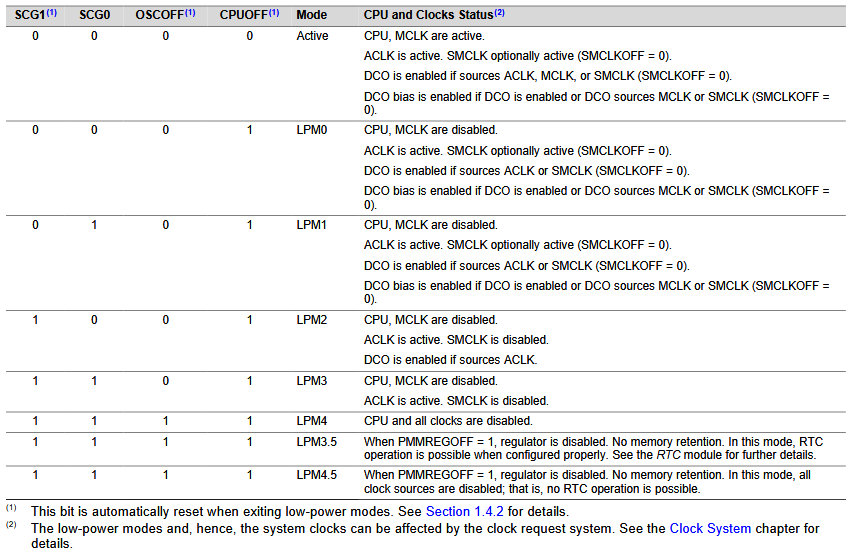
\includegraphics[width=1.0\textwidth]{../Bilder/Operating_Modes.png}
	\caption{Operating Modes \Zitat[S. 37, Kap. 1.4, Tab. 1-2]{ti:slau272d}}
	\label{fig:operation_modes}
\end{figure}

\newpage
Der Mikroprozessor besitzt 16 Kilobyte an nicht-fl\"uchtigen FRAM, sowie ein Kilobyte \Fachbegriff{Schnellster, fl\"uchtiger Speicher mit geringer Kapazit\"at, bestehend aus Flip-Flops welcher meist direkt in der \Abkuerzung{Central Processing Unit}{CPU} mit eingebaut ist.}{statischen Arbeitsspeicher}[statischer Arbeitsspeicher] (\Abkuerzung{Static Random Access Memory}{SRAM}). 

Die Versorgungsspannung betr\"agt 2 bis 3,6 Volt wobei ebenfalls verschiedene Low-Power-Modi verwendet werden k\"onnen, um den Stromverbrauch zunehmend zu minimieren. Diese beeinflussen den sp\"ateren Umgang mit Timer-Interrupts, weil sie den Energieverbrauch im Wartezustand beeinflussen. \Zitat[S. 26, Kap. 5.20]{ti:slase35c}

Des Weiteren besitzt der Chip F\"unf Interne 16-Bit Timer mit jeweils Sieben\\\NeuerBegriff{Capture and Compare} Registerbl\"ocken. Diese internen Timer stellen eine zentrale Komponente f\"ur die Realisierung pr\"aziser Zeitgesteuerter Funktionen und die Generierung von Interrupts dar, welche im nachfolgenden \Kapitel{TIMER&ISR} tiefgreifender erl\"autert werden.

Zur externen Kommunikation sind Protokolle wie \Abkuerzung{Universal Asynchronous Receiver Transmitter}{UART}, \Abkuerzung{Inter-Integrated Circuit}{I$^{2}$C} und \Abkuerzung{Serial Peripheral Interface}{SPI} integriert, welche mit 32 Programmierbaren \Abkuerzung{General Purpose Input/Output}{GPIO}-Pins angeschlossen werden k\"onnen. Kommunikationsschnittstellen sind f\"ur die Interaktion mit der Au{\ss}enwelt und Peripherieger\"aten von hoher Bedeutung. Eine detailliertere Ausarbeitung des \Fachbegriff{Serielle Schnittstelle in Mikrocontrollern von Texas Instruments, die verschiedene Kommunikationsprotokolle (\zB UART, SPI, I$^{2}$C) unterst\"utzt.}{enhanced Universal Serial Communication Interface} (\Abkuerzung{enhanced Universal Serial Communication Interface}{eUSCI}) folgt in \Kapitel{eUSCI}.\\\Zitat[S. 1, Kap. 1.1]{ti:slase35c}	

\newpage
\Abbildung{BlockDiagramm_msp430} zeigt ein vollst\"andiges Block-Diagramm des Mikroprozessors, welches noch einige weitere Eigenschaften, Funktionen und Subsysteme auflistet.\AI

\begin{figure}[h!]
	\centering
	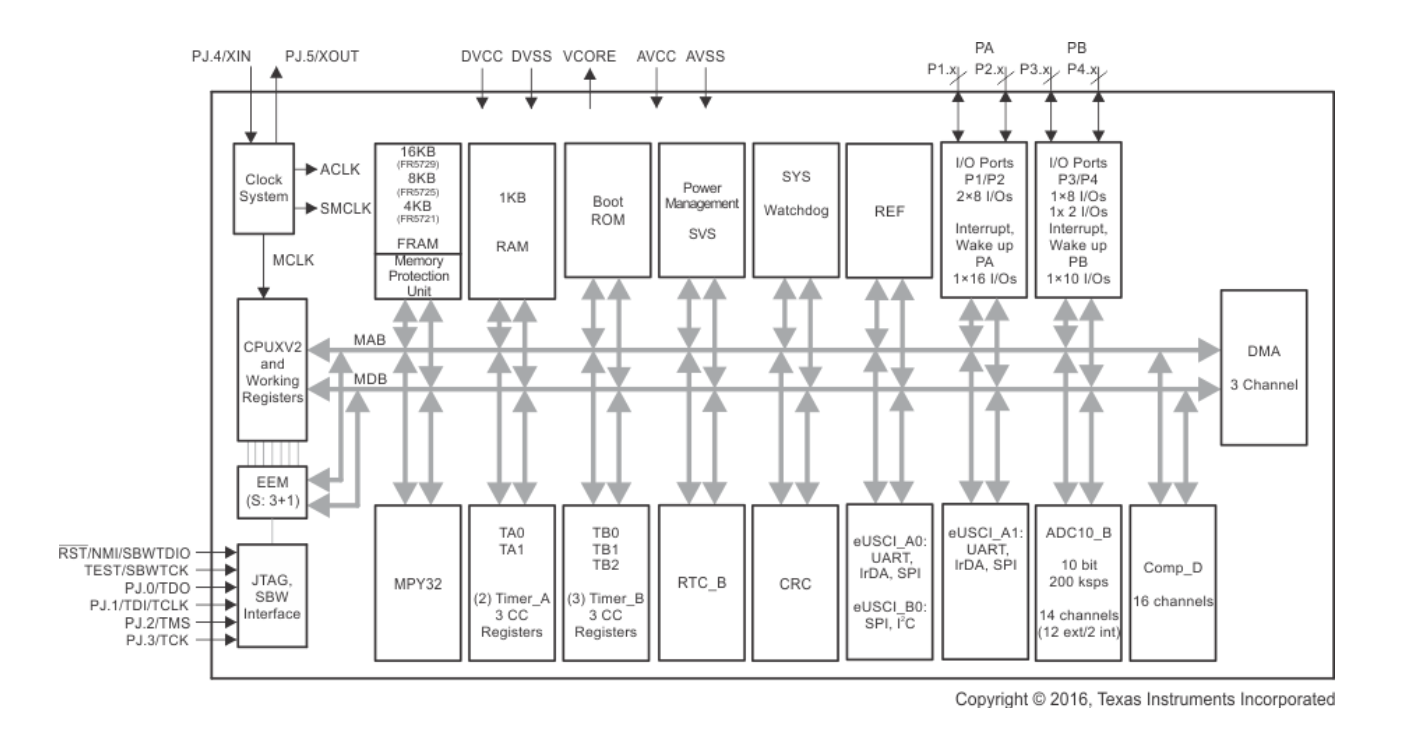
\includegraphics[width=1.0\textwidth]{../Bilder/FunctionalBlockDiagram_MSP430FR5729.png}
	\caption{Block Diagramm MSP430FR5729\\Mikrocontroller \Zitat[S. 2, Kap. 1.4]{ti:slase35c}}
	\label{fig:BlockDiagramm_msp430}
\end{figure}

\section{Timer und Interrupt Service Routinen (ISR)}
\label{sec:TIMER&ISR}

Timer und Interrupt Service Routinen (\Abkuerzung{Interrupt Service Routine}{ISR\grq s}[ISR]) stellen einen fundamentalen Baustein moderner eingebetteter Systeme dar. Sie erm\"oglichen pr\"azise, zeitgesteuerte Funktionen sowie das Reagieren auf externe Ereignisse. Womit die Realisierungen komplexer, Echtzeitsysteme m\"oglich wird. Im Folgenden wird die Timer-Architektur des MSP430FR5729 und die zugeh\"origen ISR-Mechanismen detailliert betrachtet.

Der MSP430FR5729 verf\"ugt \"uber insgesamt f\"unf 16-Bit-Timer, wovon zwei zu Typ A und drei zu Typ B geh\"oren. Timer haben vielseitige Einsatzgebiete und erm\"oglichen verschiedenste Zeitsteuerungsfunktionen. Die Unterscheidung in zwei Typen l\"asst dabei eine gr\"o{\ss}ere Vielfalt an spezifischen Konfigurationsm\"oglichkeiten zu.

\newpage
Beide Timer-Typen verf\"ugen \"uber einen gemeinsamen 16-Bit-Z\"ahler sowie sieben Capture/Compare-Register. Die korrekte Konfiguration dieser Register ist ausschlaggebend f\"ur die Implementierung verschiedenster Funktionen. Eine der beiden \"ubergeordneten Eigenschaften, die Capture-Funktionalit\"at, dient dazu, den aktuellen Z\"ahlerwert bei einem externen oder internen Ereignis pr\"azise zu erfassen. Dies ist beispielsweise n\"utzlich f\"ur die Messung von Pulsweiten oder Frequenzen. Die Compare-Funktionalit\"at hingegen erlaubt den Vergleich des aktuellen Z\"ahlerstandes mit einem in den Compare-Registern hinterlegten Wert. Bei einer \"ubereinstimmung kann eine konfigurierbare Aktion ausgel\"ost werden, wie beispielsweise das Setzen oder R\"ucksetzen eines Ausgangspins oder das Generieren eines Interrupts. Ausf\"uhrlicher beleuchtet ab \Kapitel{Timer_CaptureMode}. Die vielseitigen Einstellungsm\"oglichkeiten dieser und weiterer Register erlauben die Realisierung komplexer Zeitgesteuerter Aufgaben.\\\Zitat[S. 333, Kap. 11 \& S. 355, Kap. 12, S. 287, Kap. 8.3 \& S. 194, Kap. 6.8.2]{ti:slau272d,davies:msp430}

Die Timer des Typs B weisen im Vergleich zu dem Timer des Typs A, erweiterte Konfigurationsm\"oglichkeiten auf. Darunter f\"allt die Konfigurierbarkeit der Timer-L\"ange auf 8, 10, 12 oder 16 Bit, was eine flexible Anpassung der Z\"ahlaufl\"osung und der \"uberlaufperiode f\"ur unterschiedliche Aufl\"osungen erm\"oglicht. Zus\"atzlich sind alle Capture/Compare-Bl\"ocke doppelt gepuffert. Diese doppelte Pufferung erlaubt das Laden neuer Vergleichswerte, w\"ahrend eines aktiven Z\"ahlzyklus. Unerw\"unschte Effekte oder Inkonsistenzen in den Ausgangssignalen k\"onnen dadurch vermieden werden. Ein weiterer Unterschied besteht darin, dass die Capture/Compare-Eing\"ange asynchron zueinander sind. Somit k\"onnen sie unabh\"angig zum internen Takt des Timers operieren, was in bestimmten Szenarien die Erfassung externer Ereignisse erleichtert. \Zitat[S. 356, Kap. 12.1.1, S. 353, Kap. 8.9]{ti:slau272d, davies:msp430}

F\"ur die pr\"azise Steuerung und Ereignisbehandlung bieten die Timer verschiedene Betriebsarten, die im Folgenden n\"aher erl\"autert werden.

\newpage
\subsection{Timer Z\"ahlweisen}
\label{sec:Timer_CountMode}

Der Z\"ahlmodus, bestimmt die interne Z\"ahlweise des Timers. Die Timer unterst\"utzen typischerweise mehrere Varianten, um unterschiedlichen Anforderungen gerecht zu werden. \Zitat[S. 291, Kap. 8.3.1]{davies:msp430}

\begin{itemize}
	\item \textbf{Up Mode:} Im Up Mode (Additive Z\"ahlweise, \Vgl \Abbildung{up_mode}) beginnt der Z\"ahler bei Null und inkrementiert seinen Wert mit jedem Taktimpuls der gew\"ahlten \Fachbegriff{Eine Referenz auf ein periodisches Zeitsignal um zeitliche Abl\"aufe zu synchronisieren; typischerweise in Form von Quarzoszillatoren oder externen Taktsignalen.}{Clock-Source}. Er erreicht einen vordefinierten Maximalwert, der im Compare-Register gespeichert ist, und beginnt dann wieder von Null an zu z\"ahlen. Ein \"uberlauf-Interrupt wird generiert, sobald der Z\"ahler den Wert von \Code{CCR0} erreicht. Dieser Modus eignet sich ideal f\"ur die Erzeugung periodischer Ereignisse oder die Messung von Zeitintervallen bis zu einem bestimmten Grenzwert. Beispielsweise kann durch die Wahl einer geeigneten Clock-Source und eines passenden Wertes im Compare-Register eine pr\"azise Zeitbasis f\"ur periodische Aufgaben geschaffen werden. \Zitat[S. 337, Kap. 11.2.3.1 \& S. 359, Kap. 12.2.3.1, S. 330, Kap. 8.6]{ti:slau272d, davies:msp430}
	
	\vspace{1.25cm}
	\begin{figure}[h!]
		\centering
		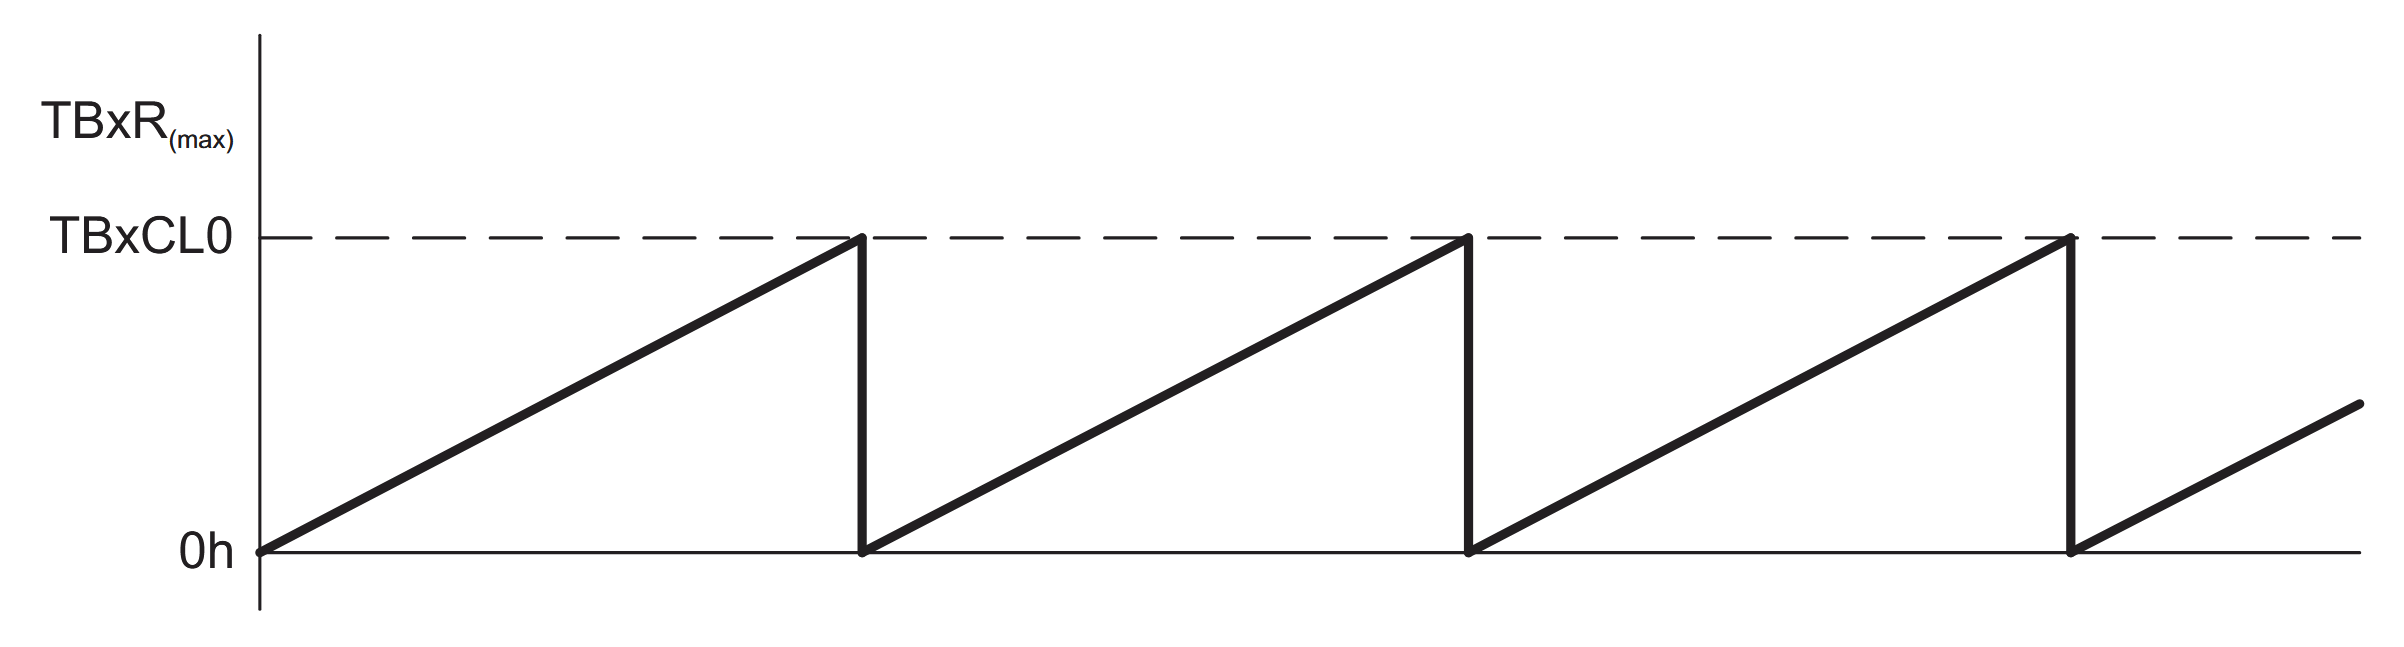
\includegraphics[width=0.85\textwidth]{../Bilder/up_mode.png}
		\caption{Up Mode \Zitat[S. 359, Abb. 12.2]{ti:slau272d}}
		\label{fig:up_mode}
	\end{figure}
	
	\newpage
	\item \textbf{Continuous Mode:} Der Continuous Mode (\Vgl \Abbildung{continuous_mode}) l\"asst den Z\"ahler von Null bis zum maximal m\"oglichen Wert (FFFFh f\"ur 16-Bit-Timer) z\"ahlen und anschlie{\ss}end wieder bei Null beginnen. Ein \"uberlauf-Interrupt wird generiert, wenn der Z\"ahler vom Wert von FFFFh auf 0 \"uberl\"auft. \Zitat[S. 338, Kap. 11.2.3.2 \& S. 360, Kap. 12.2.3.2]{ti:slau272d} Dieser Modus ist besonders n\"utzlich, wenn l\"angere, voneinander unabh\"angige Zeitintervalle zu messen sind oder eine freilaufende Zeitbasis ben\"otigt wird, um Ereignisse in Bezug auf den Z\"ahlerstand, ohne einen periodischen Neustart durch das Compare-Register, zu erfassen. \Zitat[S. 338, Kap. 11.2.3.3 \& S. 360, Kap. 12.2.3.3, S. 318, Kap. 8.5]{ti:slau272d, davies:msp430}
	
	\begin{figure}[h!]
		\centering
		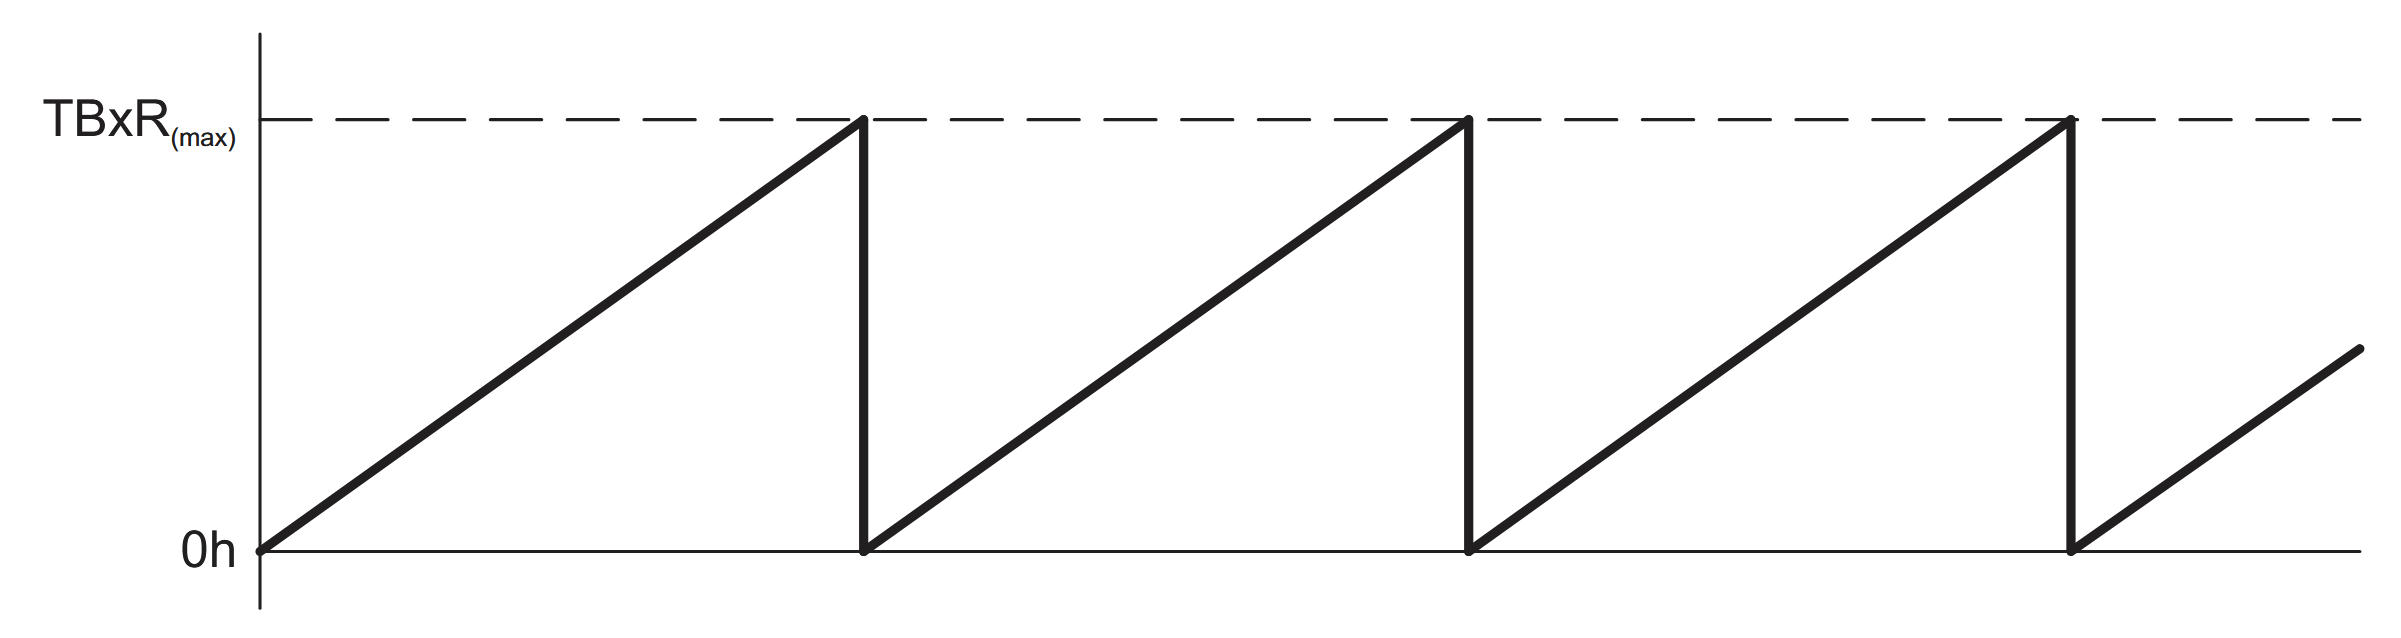
\includegraphics[width=0.75\textwidth]{../Bilder/continuous_mode.png}
		\caption{Continuous Mode \Zitat[S. 360, Abb. 12.4]{ti:slau272d}}
		\label{fig:continuous_mode}
	\end{figure}

	\item \textbf{Up/Down Mode:} Der Up/Down Mode (Auf-/Abw\"artsz\"ahlmodus, \Vgl \Abbildung{UpDown_mode}) kombiniert das Auf- und Abz\"ahlen. Der Z\"ahler beginnt bei Null, z\"ahlt Zyklisch bis zum festgelegten Wert im Compare-Register und dann wieder bis Null herunter. Ein \"uberlauf-Interrupt wird generiert, wenn der Z\"ahler den Wert von CCR0 erreicht, und ein weiterer Interrupt (sofern aktiviert) kann beim Erreichen von Null gesetzt werden. \Zitat[S. 339, Kap. 11.2.3.4 \& S. 361, Kap. 12.2.3.4]{ti:slau272d} Dieser Modus erzeugt eine symmetrische \Fachbegriff{Ein Verfahren zur Steuerung der Leistungszufuhr, bei dem die mittlere Ausgangsleistung durch Variieren des Abtastverh\"altnisses eines Rechtecksignals reguliert wird.}{Pulsweitenmodulation} (\Abkuerzung{Pulsweitenmodulation}{PWM}) und wird h\"aufig in Anwendungen zur Motorsteuerung oder zur Erzeugung pr\"aziser analoger Ausgangssignale eingesetzt. \Zitat[S. 340, Kap. 11.2.3.5 \& S. 362, Kap. 12.2.3.5, S. 349, Kap. 8.7]{ti:slau272d, davies:msp430}
	
	\begin{figure}[h!]
		\centering
		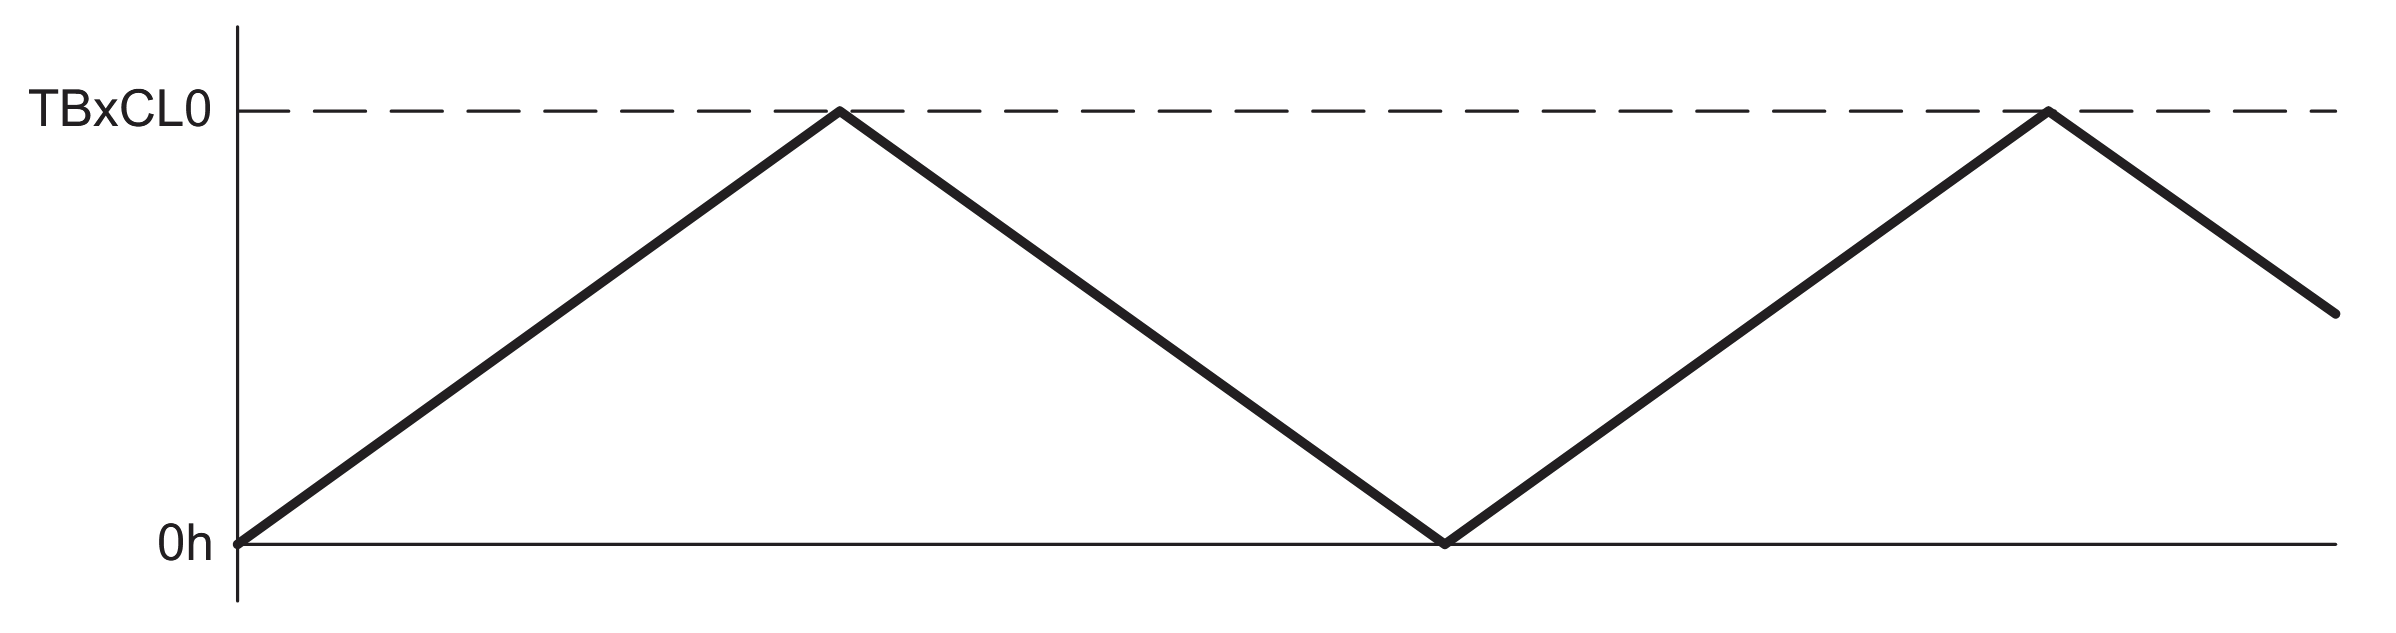
\includegraphics[width=0.75\textwidth]{../Bilder/up_down_mode.png}
		\caption{Up/Down Mode \Zitat[S. 361, Abb. 12.7]{ti:slau272d}}
		\label{fig:UpDown_mode}
	\end{figure}
\end{itemize}

Die Wahl eines geeigneten Modus h\"angt stark von der spezifischen Anwendung ab. F\"ur einfache Zeitmessungen oder periodische Aufgaben ist der Up Mode oft ausreichend, w\"ahrend der Continuous Mode f\"ur l\"angere Intervalle oder als Basis f\"ur komplexere Zeitsteuerungen dient. Der Up/Down Mode hingegen findet seine Anwendung prim\"ar in der Erzeugung von Steuersignalen.

Zur Erg\"anzug der drei Z\"ahlweisen des Timers, wird in den folgenden Kapiteln die genaue Rolle der bereits erw\"ahnten Capture-/Compare-Modi erl\"autert.

\subsection{Capture-Mode}
\label{sec:Timer_CaptureMode}

Der Capture Mode erm\"oglicht es, den aktuellen Wert des Z\"ahlers pr\"azise zu erfassen, wenn ein bestimmtes Ereignis an einem zugeh\"origen Eingangspin auftritt. Der erfasste Z\"ahlerwert wird in einem der Capture-Register (\Code{CCR0} bis \Code{CCR6}) gespeichert. Dies ist besonders n\"utzlich f\"ur die Messung von externen Signalen wie Pulsweiten, Frequenzen oder der Zeit zwischen zwei Ereignissen. Beispiele hierzu in \Abbildung{CaptureModeBeispiele}.

\vspace{1.25cm}
\begin{figure}[h!]
	\centering
	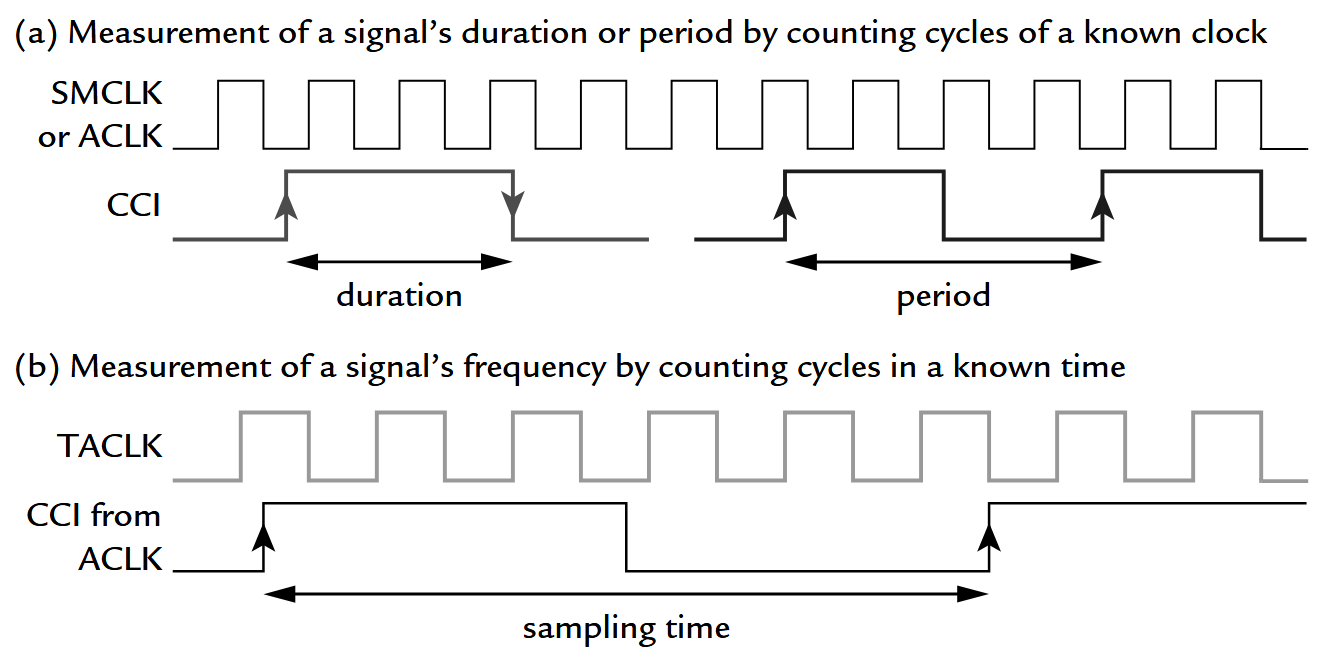
\includegraphics[width=1.0\textwidth]{../Bilder/CaptureMode_Beispiele.png}
	\caption{Capture Mode Einsatzbeispiele\\\Zitat[S. 301, Abb. 8.7]{davies:msp430}}
	\label{fig:CaptureModeBeispiele}
\end{figure}

\newpage
Die Timer des MSP430FR5729 unterst\"utzen verschiedene Capture-Modi. Diese legen fest, bei welcher Art von Signal\"anderung die Erfassung des Z\"ahlerwertes erfolgt:

\begin{itemize}
	\item \textbf{Capture on rising edge:} Sobald am zugeh\"origen Eingangspin eine steigende Flanke detektiert wird (\"ubergang von Low nach High) wird in diesem Modus der aktuelle Z\"ahlerwert in das Capture-Register geschrieben.

	\item \textbf{Capture on falling edge:} Hier erfolgt die Erfassung des Z\"ahlerwertes am Eingangspin bei einer fallenden Flanke (\"ubergang von High nach Low).

	\item \textbf{Capture on both edges:} Dieser Modus erm\"oglicht die Erfassung des Z\"ahlerwertes sowohl bei steigender als auch fallender Flanken. Dies ist besonders praktisch f\"ur die Messung von Signalperioden oder bei Relevanz beider Flanken eines Signals.
\end{itemize}

Sofern ein Interrupt im entsprechenden Capture-Register aktiviert ist, kann dieser auch Interrupts ausl\"osen. In der zugeh\"origen ISR kann der erfasste Z\"ahlerwert aus dem Capture-Register gelesen und weiterverarbeitet werden. Mehrere Capture-Register innerhalb eines Timers erm\"oglichen die Erfassung und Auswertung mehrerer aufeinanderfolgender Ereignisse, ohne dass der vorherige Wert \"uberschrieben wird. 

Die Konfiguration des Capture Mode umfasst die Auswahl des ausl\"osenden Ereignisses (Flanke) sowie \ggf die Aktivierung des Capture-Interrupts. Die erfassten Zeitstempel im Capture-Register erlauben pr\"azise Messungen und die Analyse externer Signale in eingebetteten Systemen. \Zitat[S. 340, Kap. 11.2.4.1 \& S. 362, Kap. 12.2.4.1, S. 300, Kap. 8.4]{ti:slau272d, davies:msp430}

\vspace{0.5cm}
\subsection{Compare-Mode}
\label{sec:Timer_CompareMode}

Der Compare Mode erm\"oglicht es, den aktuellen Wert des Z\"ahlers kontinuierlich mit den in den Compare-Registern \Code{CCR0} bis \Code{CCR7} hinterlegten Werten zu vergleichen. Wenn der Z\"ahlerstand mit dem Vergleichswert \"ubereinstimmt, kann \zB ein Interrupt ausgel\"ost oder ein Ausgangspin beeinflusst werden.

\newpage
Die Compare-Modi bieten verschiedene M\"oglichkeiten, wie der Ausgangspin bei einer \"ubereinstimmung beeinflusst werden soll:

\begin{itemize}
	\item \textbf{Set output on compare:} Bei einer \"ubereinstimmung des Z\"ahlerstandes mit dem Compare-Registerwert wird der zugeh\"orige Ausgangspin auf High gesetzt.

	\item \textbf{Reset output on compare:} Hier wird der Ausgangspin bei \"ubereinstimmung auf Low gesetzt.

	\item \textbf{Toggle output on compare:} In diesem Modus \"andert der Ausgangspin bei jeder \"ubereinstimmung seinen Zustand (von High nach Low oder von Low nach High).

	\item \textbf{Output High:} Der Ausgangspin wird permanent auf High gehalten.

	\item \textbf{Output Low:} Der Ausgangspin wird permanent auf Low gehalten.

	\item \textbf{Set/Reset:} In Kombination mit dem Compare-Register Null (\Code{CCR0}) kann ein PWM-Signal erzeugt werden. Beispielsweise kann der Ausgang bei Erreichen des \Code{CCR0}-Wertes gesetzt und bei Erreichen des \Code{CCRn}-Wertes zur\"uckgesetzt werden (oder umgekehrt), wobei \Code{CCRn} die Pulsweite bestimmt.
\end{itemize}

\Abbildung{OutputUnit_UpDown_Mode} zeigt eine m\"ogliche Konfiguration im Z\"ahlmodus Up/Down mit zwei Compare-Registern (\Code{TAxCCR1} \& \Code{TAxCCR2}), eingestellt auf Toggle/Set und Toggle/Reset.

\vspace{1.25cm}
\begin{figure}[h!]
	\centering
	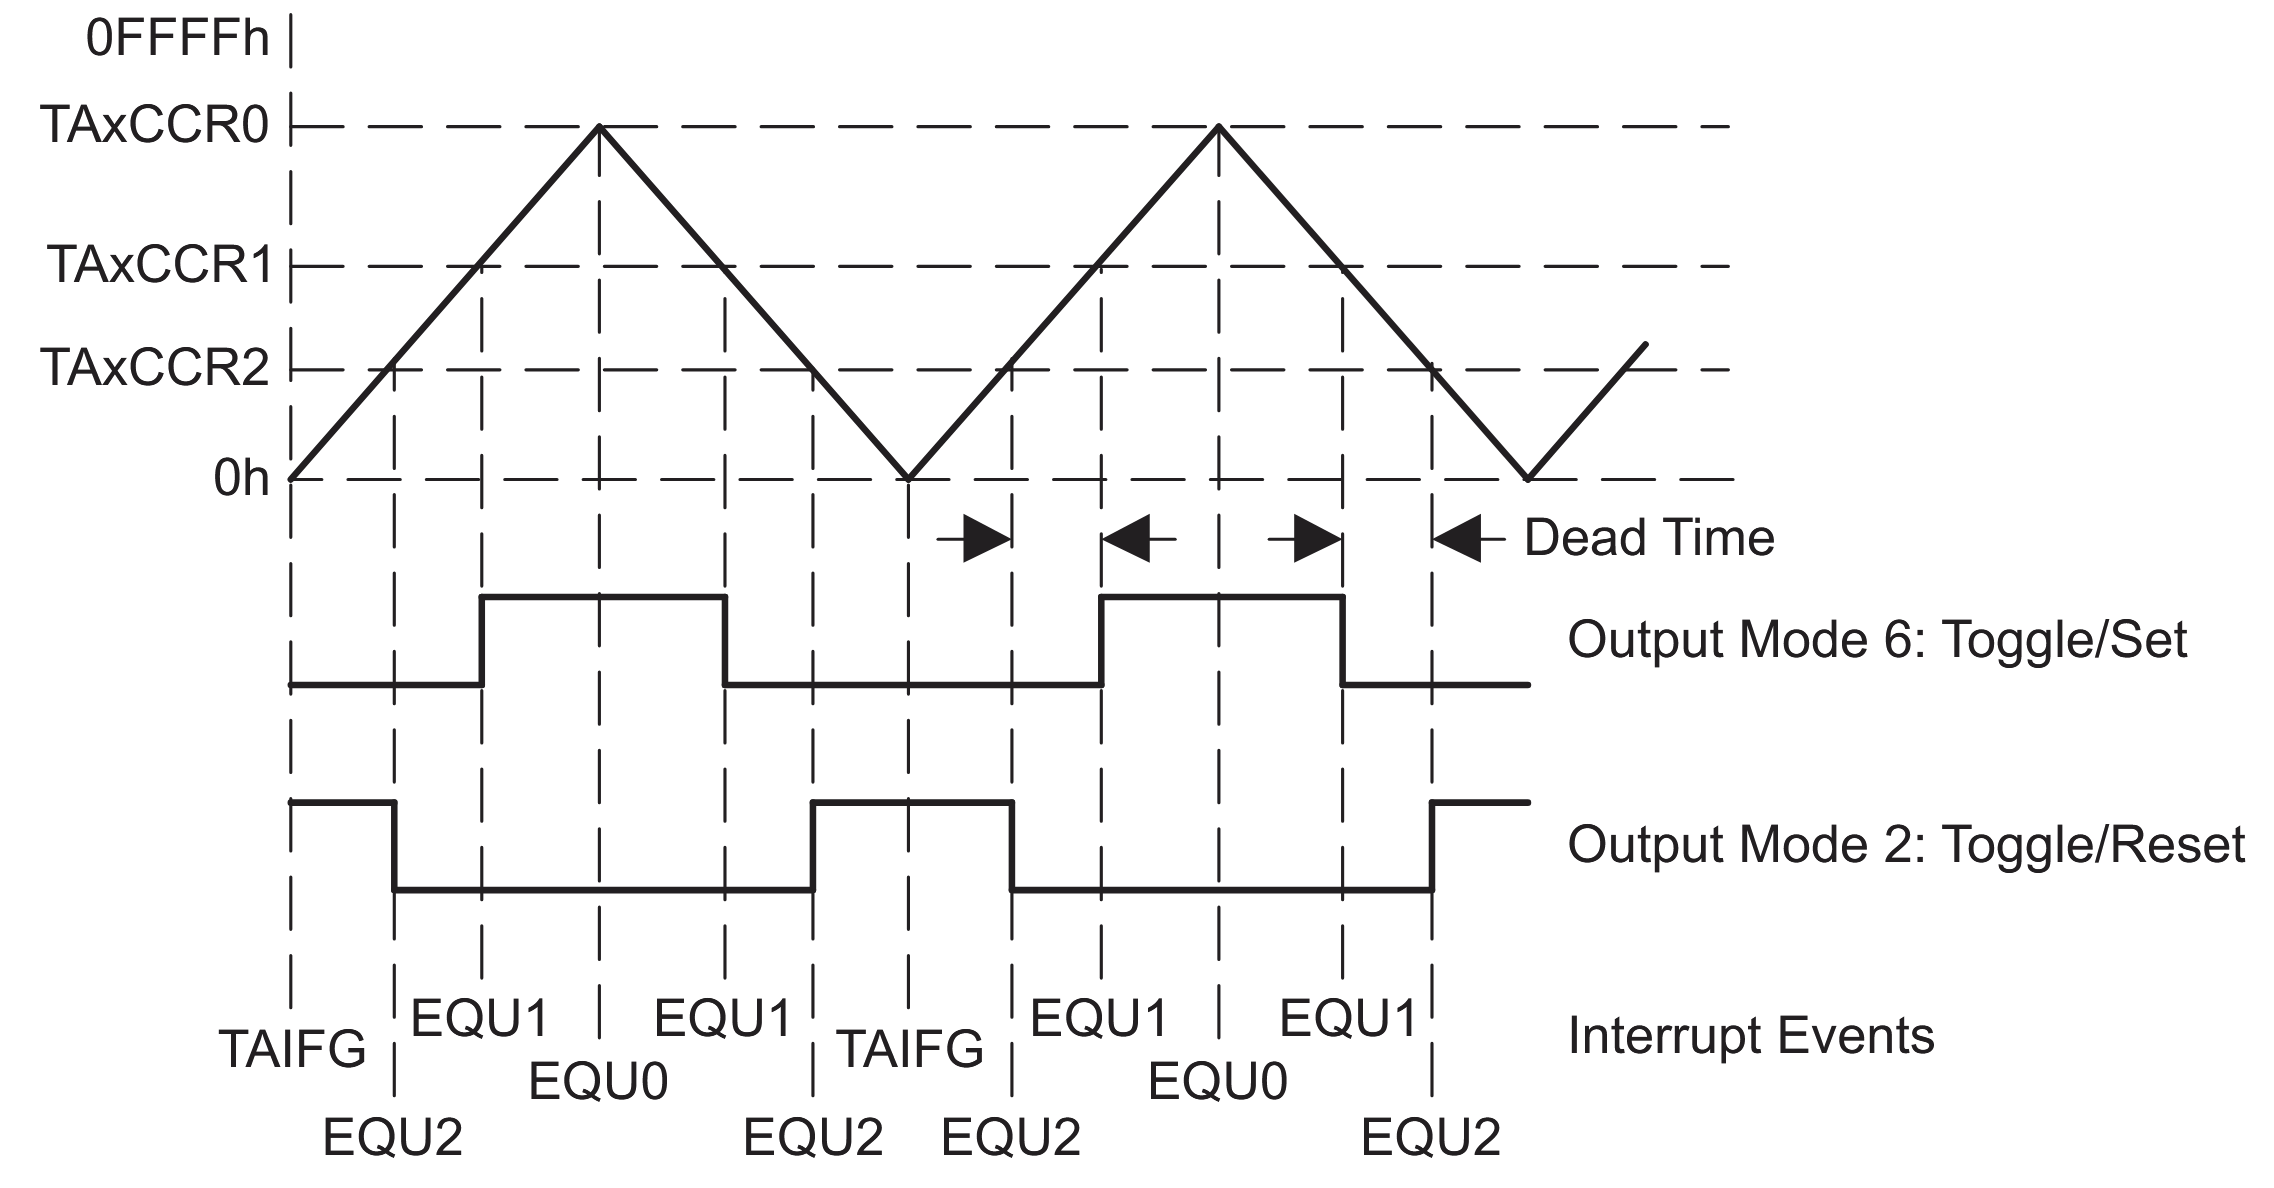
\includegraphics[width=0.95\textwidth]{../Bilder/UpDown_ModeBsp.png}
	\caption{Ausgabeeinheit im Up/Down-Modus\\\Zitat[S. 340, Abb. 11-9]{ti:slau272d}}
	\label{fig:OutputUnit_UpDown_Mode}
\end{figure}

\newpage
\"Ahnlich wie beim Capture Mode erm\"oglicht ein Interrupt der CPU, auf pr\"azise Zeitpunkte zu reagieren und entsprechende Aktionen auszuf\"uhren. Der Compare Mode ist somit ein vielseitiges Werkzeug zur Erzeugung von Steuersignalen, zur Implementierung von Zeitverz\"ogerungen oder zur Synchronisation interner Operationen mit einer pr\"azisen Zeitbasis. \Zitat[S. 342, Kap. 11.2.4.2 \& S. 364, Kap. 12.2.4.2, S. 352, Kap. 8.8]{ti:slau272d, davies:msp430}

Nachdem die verschiedenen Betriebsarten des Timers betrachtet wurden, ist es wichtig zu verstehen, wie die zugeh\"origen Register konfiguriert werden, um die gew\"unschte Funktionalit\"at zu erzielen.

\subsection{Einstellungen der Capture and Compare Register}
\label{sec:CC_Register}

Die Konfiguration der zugeh\"origen Register bestimmt ma{\ss}geblich die Funktionalit\"at der Capture- und Compare-Einheiten. Hierzu geh\"oren die Aktivierung und Deaktivierung von Interrupts, die Auswahl des Ausgangsmodus (nur f\"ur Compare) sowie die Festlegung des ausl\"osenden Ereignisses.

F\"ur jedes Capture/Compare-Register kann individuell festgelegt werden, ob ein Interrupt ausgel\"ost werden soll, wenn ein entsprechendes Ereignis eintritt. Die Aktivierung erfolgt \"uber spezifische \NeuerBegriff{Interrupt-Enable-Bits} im jeweiligen Capture/Compare-Control-Register (\Code{TAxCCTLn} oder \Code{TBxCCTLn}). Beispielsweise durch das Setzen des \Code{CCIE}-Bits auf Eins oder Null, kann die Generierung eines Interrupts bei einem Capture- oder Compare-Ereignis aktiviert \bzw deaktiviert werden. \Tabelle{tb_ccc_register} fasst alle Register, beispielhaft anhand des Timers B, mit ihren Beschreibungen zusammen.

Wie in \Kapitel{Timer_CompareMode} zum Compare-Modus erl\"autert, legen die Output-Mode-Bits (\Code{OUTMOD}) fest, wie der zugeh\"orige Ausgangspin bei einer \"ubereinstimmung des Z\"ahlerstandes mit dem Compare-Registerwert seinen Zustand ver\"andert. Die Auswahl des passenden Output-Modus ist entscheidend f\"ur die Erzeugung der gew\"unschten Ausgangssignale, wie beispielsweise bei der Pulsweitenmodulation.

Die Auswahl des ausl\"osenden Ereignisses f\"ur eine Capture- oder Compare-Operation wird ebenfalls \"uber Bits im \Code{TAxCCTLn}- oder \Code{TBxCCTLn}-Register gesteuert. F\"ur den Capture-Modus wird hier beispielsweise mit dem \Code{CM}-Bit festgelegt, ob die Erfassung bei einer steigenden, fallenden oder bei beiden Flanken des Eingangssignals erfolgen soll. 

\newpage
Im Compare-Modus legt diese Einstellung fest, unter welchen Bedingungen die Vergleichsoperation erfolgreich ist und welche Aktion (Interrupt, Ausgangssignal\"anderung) dabei erfolgt. Dies kann beispielsweise ein reiner Vergleich oder auch ein Vergleich in Kombination mit dem \"uberlauf des Z\"ahlers im Up-Modus sein.\\\Zitat[S. 351, Kap. 11.3.3 \& S. 375, Kap. 12.3.3, S. 292, Kap. 8.3.2]{ti:slau272d, davies:msp430}

\vspace{1cm}
\begin{table}[h!]
	\small
	\centering
	\begin{tabular}{|c|l|c|c|p{8cm}|}
		\hline
		\textbf{Bit} & \textbf{Feld} & \textbf{Typ} & \textbf{Reset} & \textbf{Beschreibung} \\ \hline
		15-14 & CM & RW & 0h & Capture mode \\ \hline
		13-12 & CCIS & RW & 0h & Capture/compare input select. \"Uber diese Bits wird das \Code{TBxCCRn} Input-Signal ausgew\"ahlt. \\ \hline
		11 & SCS & RW & 0h & Synchronize capture source. Dieses Bit entscheidet, ob das Capture-Input-Signal mit der Timer-Clock synchronisiert wird. \\ \hline
		10-9 & CLLD & RW & 0h & Compare latch load. Ausw\"ahlen des \glqq compare latch load events\grqq{}. \\ \hline
		8 & CAP & RW & 0h & Capture-/Compare mode \\ \hline
		7-5 & OUTMOD & RW & 0h & Output mode \\ \hline
		4 & CCIE & RW & 0h & Capture/compare interrupt enable. Aktivieren der Interrupt-Anforderung des entsprechenden \Code{CCIFG}-\FachbegriffT{Ein Flag bezeichnet in der Informatik ein einzelnes Bit oder eine boolesche Variable, die einen bin\"aren Zustand (\zB \glqq{}wahr/falsch\grqq{} oder \glqq{}aktiv/inaktiv\grqq{}) repr\"asentiert und h\"aufig zur Steuerung von Programmabl\"aufen oder zur Statusanzeige verwendet wird.}{Flag}. \\ \hline
		3 & CCI & R & Undef & Capture/compare input. Das ausgew\"ahlte Eingangssignal kann \"uber dieses Bit ausgelesen werden. \\ \hline
		2 & OUT & RW & 0h & Output. F\"ur Output-Mode \grqq 0\grqq{} kontrolliert dieses Bit den Ausgangsstatus. \\ \hline
		1 & COV & RW & 0h & Capture overflow. Dieses Bit zeigt ein \grqq capture overflow\grqq{} an. \Code{COV} muss Softwareseitig zur\"uckgesetzt werden.  \\ \hline
		0 & CCIFG & RW & 0h & Capture/compare interrupt flag \\ \hline
	\end{tabular}
	\caption{Registerbeschreibung – Capture-/Compare Register Timer B \\ \Zitat[S. 375, Tab. 12-8]{ti:slau272d}}
	\label{tab:tb_ccc_register}
\end{table}

\newpage
Die sorgf\"altige Konfiguration dieser Einstellungen in den Capture/Compare-Registern gew\"ahrleistet die Anpassung des Timers an die jeweiligen Anforderungen der Applikation.

Ein weiterer fundamentaler Aspekt der Timer-Konfiguration ist \ua die Wahl der Taktquelle, welche die Zeitbasis f\"ur den Z\"ahler und somit f\"ur alle zeitgesteuerten Operationen des Timers bestimmt.\AI

\subsection{Timer Control-Register}
\label{sec:TimerControlRegister}

Die Timer des MSP430FR5729 verwenden verschiedene interne Taktquellen, die jeweils unterschiedliche Eigenschaften aufweisen. Die prim\"aren Taktquellen sind \Fachbegriff{Niederfrequente Taktquelle in Mikrocontroller-Systemen, die typischerweise von einem Quarzoszillator gespeist wird und f\"ur energiesparende Betriebsmodi verwendet wird.}{Auxiliary Clock} (\Abkuerzung{Auxiliary Clock}{ACLK}) und \Fachbegriff{Taktgesteuertes Signal, das typischerweise f\"ur Peripherieger\"ate verwendet wird und sich aus einer frei w\"ahlbaren Taktquelle ableiten l\"asst.}{Sub-Main Clock} (\Abkuerzung{Sub-Main Clock}{SMCLK}). Auch externe Taktquellen k\"onnen zur Taktung des Timers herangezogen werden wie \zB das \Code{TACLK}/\Code{TBCLK}-Register oder der \Code{INCLK}-Pin. \\\Zitat[S. 71, Kap. 3.1, S. 163, Kap. 5.8 \& S. 289, Kap. 8.3.1]{ti:slau272d, davies:msp430}

Die Auswahl einer geeigneten \glqq Clock-Source\grqq{} f\"ur den Timer erfolgt \"uber spezifische Bits im \Code{TAxCTL} oder \Code{TBxCTL} Timer-Control-Register. Das \Code{TASSEL}-/\Code{TBSSEL}-Bit legt fest, ob der Timer von \Code{TAxCLK}/\Code{TBxCLK}, \Code{ACLK}, \Code{SMCLK} oder \Code{INCLK} getaktet wird. Diese Wahl hat einen direkten Einfluss auf die Timer-Frequenz, wobei sie nicht gleich der Frequenz der gew\"ahlten Clock-Source entsprechen muss. Durch optionale \Fachbegriff{Vorschaltglied in elektronischen Z\"ahlschaltungen oder Timern, welches die Frequenz eines Eingangssignals durch einen festen Faktor reduziert, um eine nachfolgende Verarbeitung mit geringerer Taktrate zu erm\"oglichen.}{Prescaler-Werte}[Prescaler] wie dem \Code{ID}-Bit und dem \Code{TAIDEX}-/\Code{TBIDEX}-Bit kann die Frequenz weiter individualisiert werden. \Zitat[S. 349, Kap. 11.3.1 \& S. 372, Kap. 12.3.1, S. 289, Kap. 8.3.1]{ti:slau272d, davies:msp430}

\newpage
Die Timer-Frequenz bestimmt wiederum die Zeitbasis des Timers. Eine h\"ohere Timer-Frequenz f\"uhrt zu einer feineren Zeitaufl\"osung, da der Z\"ahler schneller inkrementiert. Dies erm\"oglicht pr\"azise Zeitmessungen und die Erzeugung hochfrequenter Signale. Umgekehrt f\"uhrt eine niedrigere Frequenz zu einer gr\"oberen Zeitaufl\"osung, kann aber den Stromverbrauch reduzieren.

Ein weiteres Steuerbit, das \glqq{}Mode Control\grqq{}-Bit (\Abkuerzung{Mode Control}{MC}) steuert die -- bereits in \Kapitel{Timer_CountMode} erl\"auterten -- Z\"ahl-Modi und das \Code{TAIE}-/\Code{TBIE}-Bit steuert, ob Interrupts Ein- oder Ausgeschaltet sind.

Die Auswahl der Clock-Source, des Prescalers und weiteren Steuerbits ist daher entscheidend, um die gew\"unschte Zeitbasis, Aufl\"osung und Verhalten f\"ur den zu konfigurierenden Timer zu erreichen um die Anforderungen der jeweiligen Anwendung optimal zu erf\"ullen.

\Tabelle{tb_c_register} fasst alle weiteren Register des Timers B mit ihren Beschreibungen zusammen.\AI

\begin{table}[h!]
	\small
	\centering
	\begin{tabular}{|c|l|c|c|p{8cm}|}
		\hline
		\textbf{Bit} & \textbf{Feld} & \textbf{Typ} & \textbf{Reset} & \textbf{Beschreibung} \\ \hline
		15 & Reserved & R & 0h & Reserved. Immer als 0 gelesen. \\ \hline
		14–13 & TBCLGRP & RW & 0h & \textbf{\Code{TBxCLn}-group;} Synchrone Aktualisierung mehrerer Capture/Compare-Register. \\ \hline
		12–11 & CNTL & RW & 0h & Counter length \\ \hline
		10 & Reserved & R & 0h & Reserved. Immer als 0 gelesen. \\ \hline
		9–8 & TBSSEL & RW & 0h & clock source select \\ \hline
		7–6 & ID & RW & 0h & \textbf{Input divider;} Teilung der gew\"ahlten Clock-Source in Verbindung mit dem \Code{TBIDEX}-Register. \\ \hline
		5–4 & MC & RW & 0h & \textbf{Mode control;} Ausf\"uhrlicher in \Kapitel{Timer_CountMode} \\ \hline
		3 & Reserved & R & 0h & Reserved. Immer als 0 gelesen. \\ \hline
		2 & TBCLR & RW & 0h & Setzt \Code{TBR} und Kontroll-Logik zur\"uck. \\ \hline
		1 & TBIE & RW & 0h & Timer\_B interrupt enable \\ \hline
		0 & TBIFG & RW & 0h & Timer\_B interrupt flag \\ \hline
	\end{tabular}
	\caption{Registerbeschreibung – Control Register Timer B\\\Zitat[S. 372, Tab. 12-6]{ti:slau272d}}
	\label{tab:tb_c_register}
\end{table}

\newpage
\subsection{Zusammenfassung der Einsatzm\"oglichkeiten}
\label{sec:TimerEinsatzmoeglichkeiten}

Die detaillierte Auseinandersetzung mit der Timer-Architektur des MSP430FR5729 verdeutlicht die Flexibilit\"at und Leistungsf\"ahigkeit dieser Peripheriekomponente. Die Unterscheidung zwischen Timer des Typs A und B, die verschiedenen Betriebsarten (Z\"ahlmodus und Capture/Compare) sowie die vielf\"altigen Einstellm\"oglichkeiten der Steuerregister und die Auswahl der Taktquelle er\"offnen ein breites Spektrum an Anwendungsm\"oglichkeiten in eingebetteter Software.

Analog zur \"Ubersicht \glqq What Timer Where?\grqq{} von John H. Davies lassen sich die prim\"aren Einsatzgebiete der Timer des MSP430FR5729 wie folgt zusammenfassen: \Zitat[S. 356, Kap. 8.10]{davies:msp430}

\begin{itemize}
	\item \textbf{Zeitmessung und Zeitbasis:} Unabh\"angig vom Timer-Typ k\"onnen alle als eine pr\"azise Zeitbasis dienen. Durch die Wahl einer geeigneten Clock-Source und passender Prescaler-Werte lassen sich genaue Zeitintervalle festlegen. Dies ist fundamental f\"ur das Zeitmanagement innerhalb des Mikrocontrollers und die Synchronisation mit externen als auch Internen Ereignissen. Timer A eignet sich f\"ur grundlegende Zeitsteuerungsaufgaben, w\"ahrend Timer B durch seine flexiblere Konfiguration eine genauere Anpassung erm\"oglicht.

	\item \textbf{Ereigniserfassung (Capture):} Die Capture-Funktionalit\"at erm\"oglicht eine pr\"azise Erfassung des Zeitpunkts externer -- oder \ggf auch interner -- Ereignisse. Diese Erfassung spielt eine zentrale Rolle bei Anwendungen wie der Pulsweitenmessung, der Frequenzmessung oder der Detektion von Ankunftszeiten. Die M\"oglichkeit, sowohl steigende, fallende Flanken oder auch beide zu erfassen, erweitert den Anwendungsbereich in vielen verschiedenen Szenarien.

	\item \textbf{Signalerzeugung (Compare/PWM):} Die Compare-Einheiten in Verbindung mit den verschiedenen Ausgangsmodi erlauben die Generierung pr\"aziser Ausgangssignale. Dies ist besonders relevant f\"ur die Pulsweitenmodulation, die zur Steuerung von Motoren, zur Dimmung von LEDs oder zur Erzeugung analog wirkender Signale eingesetzt wird. Der Up/Down Mode des Count-Modus in Kombination mit den Compare-Registern des Timer B bietet hierbei besonders flexible M\"oglichkeiten zur Erzeugung verschiedenster PWM-Signale.

	\newpage
	\item \textbf{Interrupt-Steuerung und Task-Rotation:} Sowohl Capture- als auch Compare-Ereignisse l\"osen Interrupts aus. Dies erm\"oglicht eine effiziente Reaktion des Mikrocontrollers auf zeitgesteuerte Ereignisse oder Signale, ohne die kontinuierliche abfrage des Timer-Status. Die pr\"azise Interrupt-Generierung tr\"agt ma{\ss}geblich zur Realisierung reaktiver und effizienter eingebetteter (Echtzeit-) Systeme bei.
\end{itemize}

Zusammenfassend zeigt sich der grundlegende Aufbau eines Timers in Anlehnung an Abbildung 8.5 und Abbildung 8.16 aus Davies' Buch, wie folgt:

Ein Timer besteht im Kern aus einem Z\"ahler (\Kapitel{Timer_CountMode}), der durch eine ausgew\"ahlte Clock-Source (\Kapitel{TimerControlRegister}) in definierten Schritten inkrementiert oder dekrementiert wird. Der Z\"ahler arbeitet entsprechend der gew\"ahlten Betriebsart.

Zus\"atzlich verf\"ugt der Timer \"uber Sieben Capture/Compare-Kan\"ale. Jeder Kanal beinhaltet mindestens ein Capture/Compare-Register sowie die zugeh\"orige Steuereinheit.

Im Capture Mode (\Kapitel{Timer_CaptureMode}) wird der aktuelle Wert des Z\"ahlers in das \Code{CCRx}-Register geschrieben, wenn ein durch die Steuereinheit ausgew\"ahltes Ereignis (\zB Flanke an einem Eingangspin) eintritt.

Im Compare Mode (\Kapitel{Timer_CompareMode}) wird der aktuelle Wert des Z\"ahlers kontinuierlich mit dem Wert im \Code{CCRx}-Register verglichen. Bei einer \"Ubereinstimmung l\"ost die Steuereinheit eine konfigurierte Aktion aus -- wie beispielsweise das Setzen/R\"ucksetzen/Toggeln eines zugeh\"origen Ausgangspins oder die Generierung eines Interrupts -- sofern der Interrupt in der Steuereinheit aktiviert ist.

Die Steuereinheit erm\"oglicht die Konfiguration des jeweiligen Kanals, einschlie{\ss}lich der Auswahl des Capture/Compare-Modus, des ausl\"osenden Ereignisses, des Ausgangsmodus und der Aktivierung/Deaktivierung des Interrupts.

Das Blockdiagramm in \Abbildung{BlockDiagramm_Timer} zeigt Timer B mit seinen grundlegenden Komponenten und deren Zusammenspiel. Die flexiblen Konfigurationsm\"oglichkeiten dieser Bl\"ocke erm\"oglicht die Realisierung einer Vielzahl von Zeitsteuerungs- und Signalverarbeitungsaufgaben.

\newpage
\vspace{1cm}
\begin{figure}[h!]
	\centering
	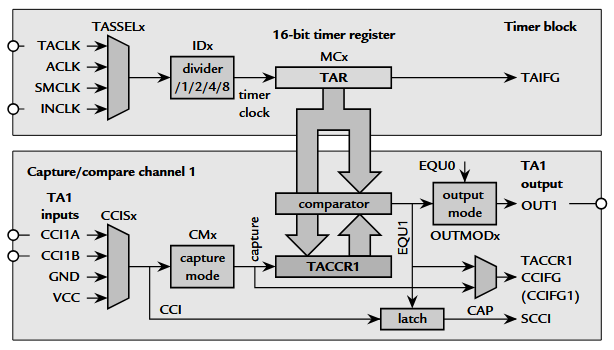
\includegraphics[width=1.0\textwidth]{../Bilder/BlockDiagram_TimerB.png}
	\caption{Timer B Block \& Capture/Compare Channel 1\\\Zitat[S. 355, Kap. 8.16]{davies:msp430}}
	\label{fig:BlockDiagramm_Timer}
\end{figure}

\section{Enhanced Universal Serial Communication Interface (eUSCI)}
\label{sec:eUSCI}

Das eUSCI ist eine vielseitige und flexible serielle Peripheriekomponente des MSP430FR5729. Sie erm\"oglicht die Kommunikation mit externen Ger\"aten und Systemen \"uber zahlreiche Schnittstellen und Protokolle. Auch Sensoren, Aktoren und Speichermedien verbindet das System auf diese Weise. Dieses Kapitel beleuchtet die Architektur des \Fachbegriff{Ein Interface bezeichnet in der Informatik eine definierte Schnittstelle, \"uber die Komponenten eines Softwaresystems miteinander kommunizieren k\"onnen, ohne deren interne Implementierung zu kennen.}{Interfaces}[Interface], seine verschiedenen Betriebsmodi und Konfigurationsm\"oglichkeiten bereitgestellter Kommunikationstechnologien.

Der MSP430FR5729 besitzt zwei Kommunikationskan\"ale, die die folgenden Kapitel n\"aher beschreiben.

\newpage
\subsection{Die eUSCI-Architektur}
\label{sec:eUSCI_Architektur}

Jede Form der \Fachbegriff{Die \"Ubertragung von Datenbitfolgen \"uber eine einzelne Leitung, wobei die Bits nacheinander (also \glqq seriell\grqq{}) gesendet werden. Sie wird h\"aufig bei einfachen oder ressourcenschonenden Datenverbindungen eingesetzt, \zB \"uber UART, SPI oder I$^{2}$C.}{Seriellen Kommunikation}[Serielle Kommunikation] basiert auf einem Taktgeber. Der zentrale Unterschied zwischen Protokollen liegt im Timing: Wann gestattet der Taktgeber dem Sender das Schreiben des n\"achsten Bits auf einen Ausgangskanal und dem Empf\"anger das Lesen des kommenden Bits. Dabei gibt es Synchrone und Asynchrone Ans\"atze, weshalb zwei Kommunikationskan\"ale bereitgestellt werden.\\\Zitat[S. 494, Kap. 10]{davies:msp430}

Beim MSP430FR5729 ist der Kommunikationskanal vom Typ-B f\"ur Synchrone Daten\"ubertragung optimiert, w\"ahrend Kanal A vorrangig f\"ur asynchrone \"Ubertragungsverfahren vorgesehen ist. \Zitat[S. 496, Kap. 10.1.2]{davies:msp430}

Der wesentliche Unterschied zwischen diesen beiden \"Ubertragungsarten besteht darin, ob das Taktsignal ebenfalls mit \"ubertragen wird. Bei der synchronen Kommunikation, wie sie etwa mit den Protokollen SPI oder I$^{2}$C erfolgt, wird dieses Taktsignal explizit mitgef\"uhrt. Im Gegensatz dazu kommt das UART-Protokoll ohne ein separates Taktsignal aus, da Sender und Empf\"anger \"uber eine gemeinsame \Fachbegriff{Bezeichnet die Anzahl der Signal\"anderungen (Symbole) pro Sekunde in einem \"Ubertragungskanal. Sie bestimmt somit die \"Ubertragungsgeschwindigkeit, ist aber nicht zwingend identisch mit der Bitrate, da pro Symbol mehrere Bits codiert sein k\"onnen.}{Baudrate} synchronisiert sind. \Zitat[S. 494, Kap. 10]{davies:msp430}

Entsprechend ist der universelle Kommunikationskanal vom Typ B (\Abkuerzung{enhanced Universal Serial Communication Interface Type B}{eUSCI\_B}{}) speziell auf die Anforderungen synchroner Protokolle wie SPI und I$^{2}$C ausgelegt. Das \Abkuerzung{enhanced Universal Serial Communication Interface Type A}{eUSCI\_A}{}-Modul hingegen unterst\"utzt prim\"ar die UART-Kommunikation, kann jedoch dar\"uber hinaus auch eine asynchrone Variante des SPI-Protokolls abbilden.\\\Zitat[S. 496, Kap. 10.1.2]{davies:msp430}

\newpage
\begin{table}[h!]
	\small
	\centering
	\begin{tabular}{|l|c|c|}
		\hline
		\textbf{Funktion} & \textbf{eUSCI\_A} & \textbf{eUSCI\_B} \\\hline
		UART (asynchron) & \checkmark & -- \\\hline
		SPI (synchron) & \checkmark (Master/Slave) & \checkmark (Master/Slave) \\\hline
		SPI (asynchron, nur TX) & \checkmark & -- \\\hline
		I\textsuperscript{2}C (synchron) & -- & \checkmark (Master/Slave) \\\hline
		\Abkuerzung{Local Interconnected Network}{LIN}-kompatibel (\FachbegriffT{Serieller Kommunikationsstandard, zur kosteng\"unstigen Vernetzung von Mikrocontrollern in Fahrzeugen, insbesondere bei weniger zeitkritischen Steuerger\"aten.\Zitat{csselectronics_lin}}{Local Interconnected Network}) & \checkmark & -- \\\hline
		Automatische Baudratenerkennung (UART) & \checkmark & -- \\\hline
		Adress- und Broadcast-Modus (I$^{2}$C) & -- & \checkmark \\\hline
		Multimaster-Unterst\"utzung (I$^{2}$C) & -- & \checkmark \\\hline
	\end{tabular}
	\caption{Funktionsvergleich der eUSCI-Module des MSP430FR5729\\\Zitat[Kap. 18, 19, 20, S. 493, Kap. 10]{ti:slau272d, davies:msp430}}
	\label{tab:eusci-vergleich}
\end{table}

\Tabelle{eusci-vergleich} fasst nochmals alle Eigenschaften beider Kan\"ale zusammen und stellt sie gegen\"uber. Wobei tiefgreifendere protokollspezifische Funktionen in den entsprechenden Unterkapiteln n\"aher betrachtet werden.

\subsection{Einordnung vorhandener Kommunikationsschnittstellen}
\label{sec:Einordnung_Schnittstellen}

Diese Arbeit entwickelt eine interruptgesteuerte Benutzerschnittstelle. Die Evaluation daf\"ur geeigneter Protokolle zur Interaktion mit externen \Abkuerzung{Personal Computer}{PC} Systemen bestimmt ma{\ss}geblich den weiteren Verlauf des Projekts. Daher ordnet die Arbeit die verf\"ugbaren seriellen Protokolle ein, um im weiteren Verlauf gezielt auf jene Technologie eingehen zu k\"onnen, welche im Kontext der Arbeit von praktischer Relevanz ist.

Die Kommunikation \"uber synchrone Protokolle wie I$^{2}$C und SPI eignen sich besonders gut f\"ur den Datenaustausch zwischen einem Mikrocontroller und seinen Peripherieger\"aten oder weiteren Mikrocontrollern im Master-Slave-Verh\"altnis. Die Wahl der Technologie richtet sich unter anderem nach der Anzahl beteiligter Ger\"ate sowie der Distanz zu den Kommunikationspartnern. Weitere technische Unterschiede dieser Protokolle sind in \Tabelle{synchrone_protokolle} aufgelistet.

\newpage
\begin{table}[h!]
	\small
	\centering
	\begin{tabular}{|p{4.5cm}|p{4.5cm}|p{4.5cm}|}
		\hline
		\textbf{Kriterium} & \textbf{SPI} & \textbf{I$^{2}$C} \\\hline
		\textbf{Signalleitungen} & 4 Leitungen: SCLK, MOSI, MISO, CS (pro Slave) & 2 Leitungen: SCL (Takt), SDA (Daten) \\\hline
		\textbf{Adressierung} & Keine; Slaves \"uber eigene Chip Selects (CS) & Ja; \"uber 7- oder 10-Bit-Adresse auf dem Bus \\\hline
		\textbf{Daten\"ubertragung} & \FachbegriffT{Gleichzeitige Daten\"ubertragung in beide Richtungen}{Vollduplex} m\"oglich & \FachbegriffT{Daten\"ubertragung zu einem Zeitpunkt nur in eine Richtung m\"oglich}{Halbduplex} \\\hline
		\textbf{Taktfrequenz} & Bis > 10\,MHz (ger\"ateabh\"angig) & Typisch 100\,kHz, 400\,kHz, bis 3.4\,MHz (High-Speed) \\\hline
		\textbf{Komplexit\"at des Protokolls} & Einfach, ohne Start-/Stopp- oder ACK-Signale & H\"oher, mit Start-/Stoppbedingungen und Acknowledgements \\\hline
		\textbf{Multimaster-Unterst\"utzung} & Nein (standardm\"a{\ss}ig) & Ja \\\hline
		\textbf{Skalierbarkeit (Anzahl Ger\"ate)} & Eingeschr\"ankt, abh\"angig von verf\"ugbaren CS-Leitungen & Hoch, bis zu 128 Ger\"ate durch Adressierung \\\hline
		\textbf{Typische Einsatzgebiete} & Hochgeschwindigkeits-kommunikation (\zB SD-Karten, Displays) & Niedriggeschwindigkeits-Komponenten (\zB Sensoren, EEPROMs) \\\hline
		\textbf{Leitungsl\"ange / St\"oranf\"alligkeit} & Gut f\"ur kurze, direkte Verbindungen & H\"ohere Anf\"alligkeit f\"ur St\"orungen und Begrenzung durch Leitungskapazit\"at \\\hline
	\end{tabular}
	\caption{Vergleich der synchronen seriellen Protokolle SPI und I$^{2}$C\\\Zitat[S. 497, Kap. 10.2, S. 534, Kap. 10.7]{davies:msp430}}
	\label{tab:synchrone_protokolle}
\end{table}

Zusammenfassend zeigt sich, dass die synchrone Daten\"ubertragung sich nur bedingt f\"ur die Kommunikation mit einem auf Windows oder Linux basierenden System eignet. Im Gegensatz dazu sind asynchrone Protokolle wie UART f\"ur diese Art der Anwendung deutlich besser geeignet, wie der folgende Abschnitt beschreibt. 

Das UART-Protokoll zeichnet sich nicht nur durch eine einfache Implementierung aus, sondern ist auch \"au{\ss}erst robust und ressourcenschonend -- Eigenschaften, die insbesondere bei modularen, \Fachbegriff{Automatische Erkennung und Integration von Komponenten in ein System ohne manuelle Konfiguration}{Plug-and-Play-f\"ahigen}[Plug-and-Play] Systemkomponenten entscheidend sind. Der Verzicht auf eine gemeinsame Taktleitung erlaubt eine Punkt-zu-Punkt-Verbindung mit vergleichsweise geringen Hardwareanforderungen. 

\newpage
Diese Vorteile gelten gleicherma{\ss}en f\"ur die gegen\"uberliegende Seite der Schnittstelle: Alle g\"angigen Betriebssysteme wie Windows, Linux oder macOS stellen standardm\"a{\ss}ig Treiber f\"ur die asynchrone serielle Daten\"ubertragung bereit. Unter Windows erfolgt dies beispielsweise \"uber sogenannte \NeuerBegriff{COM-Ports}, w\"ahrend unter Linux Schnittstellen wie \NeuerBegriff{/dev/ttySx} oder \NeuerBegriff{/dev/ttyUSBx} verwendet werden. \Zitat{microsoft_serial, linux_kernel_docs}

Im Falle des MSP430FR5729 erfolgt die UART-Kommunikation zus\"atzlich interruptgesteuert. Dies erlaubt es, eingehende Daten \"uber eine eigens definierte ISR zu verarbeiten, was eine latenzarme, gleichzeitig jedoch energieeffiziente Verarbeitung erm\"oglicht. \Zitat[S. 574, Kap. 10.12]{davies:msp430}

Aus diesen Gr\"unden stellt UART die technisch sinnvollste Wahl f\"ur die Kommunikation zwischen dem MSP430FR5729 und einem PC mit Windows, Linux oder macOS dar. Das Protokoll erlaubt eine minimalinvasive, betriebssystemkompatible und energieeffiziente Verbindung. Im weiteren Verlauf wird die asynchrone universelle serielle Schnittstelle mit dem UART Protokoll detaillierter betrachtet.\AI

\subsection{eUSCI\_A Modul: UART-Modus (Asynchrone Kommunikation)}
\label{sec:eUSCI_UART}

F\"ur ein tiefgreifendes Verst\"andnis des Zusammenspiels zwischen dem Interface und dem UART-Protokoll ist es unerl\"asslich, zun\"achst die fundamentalen technischen Aspekte, notwendige Register und charakteristische Merkmale zu erl\"autern.

\subsubsection{Informations\"ubertragung}
\label{sec:UART_uebertragung}

Die Baudrate, wie in \Kapitel{eUSCI_Architektur} bereits er\"ortert, fungiert als entscheidender Synchronisationsmechanismus f\"ur asynchrone Daten\"ubertragungen. Dies impliziert, dass Sender und Empf\"anger sich zwar nicht an ein pr\"azises Timing f\"ur die \"Ubertragung einzelner Bits halten m\"ussen, jedoch eine \"Ubereinstimmung hinsichtlich der Frequenz zur \"Ubertragung ganzer Bl\"ocke -- typischerweise Bytes oder Zeichen -- erforderlich ist. 

\newpage
\Abbildung{uart_send} visualisiert beispielhaft die \"Ubertragung zweier Bl\"ocke, die jeweils durch ein Start-Bit (\Abkuerzung{Start-Bit}{ST}) eingeleitet und durch ein Stop-Bit (\Abkuerzung{Stop-Bit}{SP}) abgeschlossen werden. Durch die Verwendung dieser Rahmenbits ergibt sich bei einer Konfiguration von acht Datenbits eine Netto-Datenrate von 8/10 der Brutto-\"Ubertragungsrate. Das bedeutet, dass von zehn \"ubertragenen Bits acht Bits die eigentliche Nutzinformation darstellt. Es gibt auch die M\"oglichkeit, flexibel auf unterschiedliche Baudraten zu reagieren. Vorausschauend sei erw\"ahnt, dass die in \Kapitel{auto_baud} erl\"auterte automatische Baudraten-Erkennung die Kommunikation mit mehreren Partnern bei unterschiedlichen Baudraten erlaubt. \Zitat[S. 576, Kap. 10.12.1]{davies:msp430, riverdi_baudrate}

\begin{figure}[h!]
	\centering
	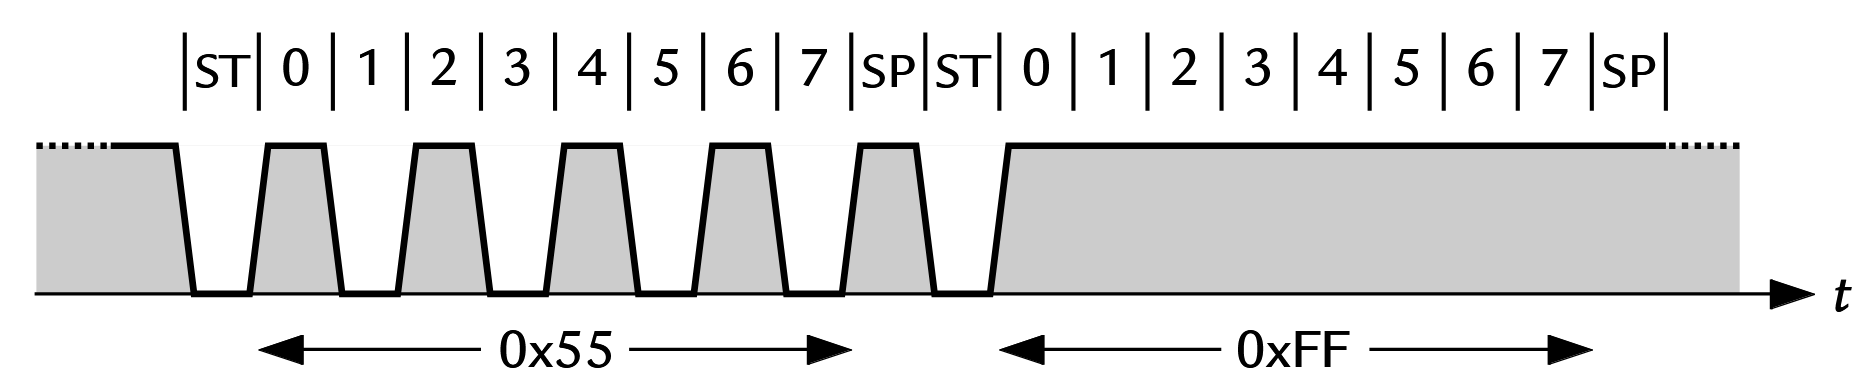
\includegraphics[width=1.0\textwidth]{../Bilder/Baudrate.png}
	\caption{UART \"ubertragung der Werte 0x55 und 0xFF\\\Zitat[S. 576, Abb. 10.18]{davies:msp430}}
	\label{fig:uart_send}
\end{figure}

Die einzelnen Bits innerhalb eines Datenblocks werden mittels des \Fachbegriff{Bin\"ares Leitungscodierungsverfahren, bei dem der Signalpegel w\"ahrend eines Bitintervalls konstant bleibt und nicht zwischen den Bits auf einen Nullpegel zur\"uckkehrt}{Non-Return-to-Zero-Verfahrens}[Non-Return-to-Zero] (\Abkuerzung{non-return to zero}{NRZ}) kodiert und \"ubertragen. Eine typische Baudrate f\"ur eingebettete Systeme betr\"agt 9600 Baud, obgleich auch h\"ohere Frequenzen zur beschleunigten Daten\"ubertragung Anwendung finden k\"onnen. \Zitat{riverdi_baudrate}

Drei Leitungen stellen \"ublicherweise die physikalische Verbindung zwischen zwei Parteien her. Eine Leitung f\"ur jede Kommunikationsrichtung (\Abkuerzung{Transmit Data}{TxD} zu \Abkuerzung{Receive Data}{RxD}) und eine f\"ur die gemeinsame Masse. Dies erm\"oglicht eine \NeuerBegriff{Vollduplex-Kommunikation}, bei der beide Seiten gleichzeitig und unabh\"angig voneinander Daten senden und empfangen k\"onnen. Voraussetzungen hierf\"ur sind separate Sende-/Empfangsschieberegister sowie dedizierte Puffer -- \Code{UCAxRXBUF} als Empfangs- und \Code{UCAxTXBUF} als Sendepuffer -- f\"ur beide Kommunikationsrichtungen in der Hardware des Interfaces. \\\Zitat[S. 499, Kap. 18.4.6 \& 18.4.7]{ti:slau272d}

\newpage
Beim Empfang eines UART-Blocks ergibt sich folgender Ablauf:

\begin{enumerate}
	\item Beginn der Zeitmessung mit der fallender Flanke, die das Startbit einleitet.
	\item Abtastung des Eingangs nach einer halben Bitperiode zur Best\"atigung eines g\"ultigen Startbits.
	\item Weitere Abtastung nach einer vollst\"andigen Bitperiode zur Erfassung des ersten Datenbits (\Abkuerzung{Least Significant Bit}{LSB}).
	\item Wiederholung dieses Vorgangs f\"ur alle 8 Datenbits bis zum h\"ochstwertigen Bit (\Abkuerzung{Most Significant Bit}{MSB}).
	\item Abschlie{\ss}ende Abtastung nach einer weiteren Bitperiode zur \"Uberpr\"ufung des Stopbits (\Fachbegriff{Bezeichnet in der Digitaltechnik einen Spannungszustand, der \"uber einer definierten Schaltschwelle liegt.}{High-Pegel} erwartet). Liegt stattdessen ein \Fachbegriff{Bezeichnet in der Digitaltechnik einen Spannungszustand, der unter einer definierten Schaltschwelle liegt.}{Low-Pegel} vor, wird ein Framing-Fehler erkannt.
\end{enumerate}

\Abbildung{uart_uebertragung} visualisiert diesen Empfangsprozess unter Verwendung einer sogenannten \Fachbegriff{Bestimmt den Zeitpunkt der Abtastung eingehender Bits; sie wird \"ublicherweise aus einer \"ubergeordneten Taktquelle (\zB SMCLK) abgeleitet und beeinflusst ma{\ss}geblich die Genauigkeit der Daten\"ubertragung.}{\glqq sampling clock\grqq{}}[sampling clock]. Diese Abtastfrequenz ist \"ublicherweise um den Faktor 16 h\"oher als die konfigurierte Baudrate. Das \Fachbegriff{Oversampling bezeichnet das Verfahren, bei dem ein Signal mit einer h\"oheren Abtastrate als der Abtastgrenze (Nyquist-Rate) digitalisiert wird, um Rauscheinfl\"usse zu reduzieren und die Signalqualit\"at zu verbessern.}{Oversampling} ist notwendig um das eintreffende Start-Bit zuverl\"assig und zeitnah auch zwischen den regul\"aren Bit-Takten detektieren zu k\"onnen.

\newpage
\begin{figure}[h!]
	\centering
	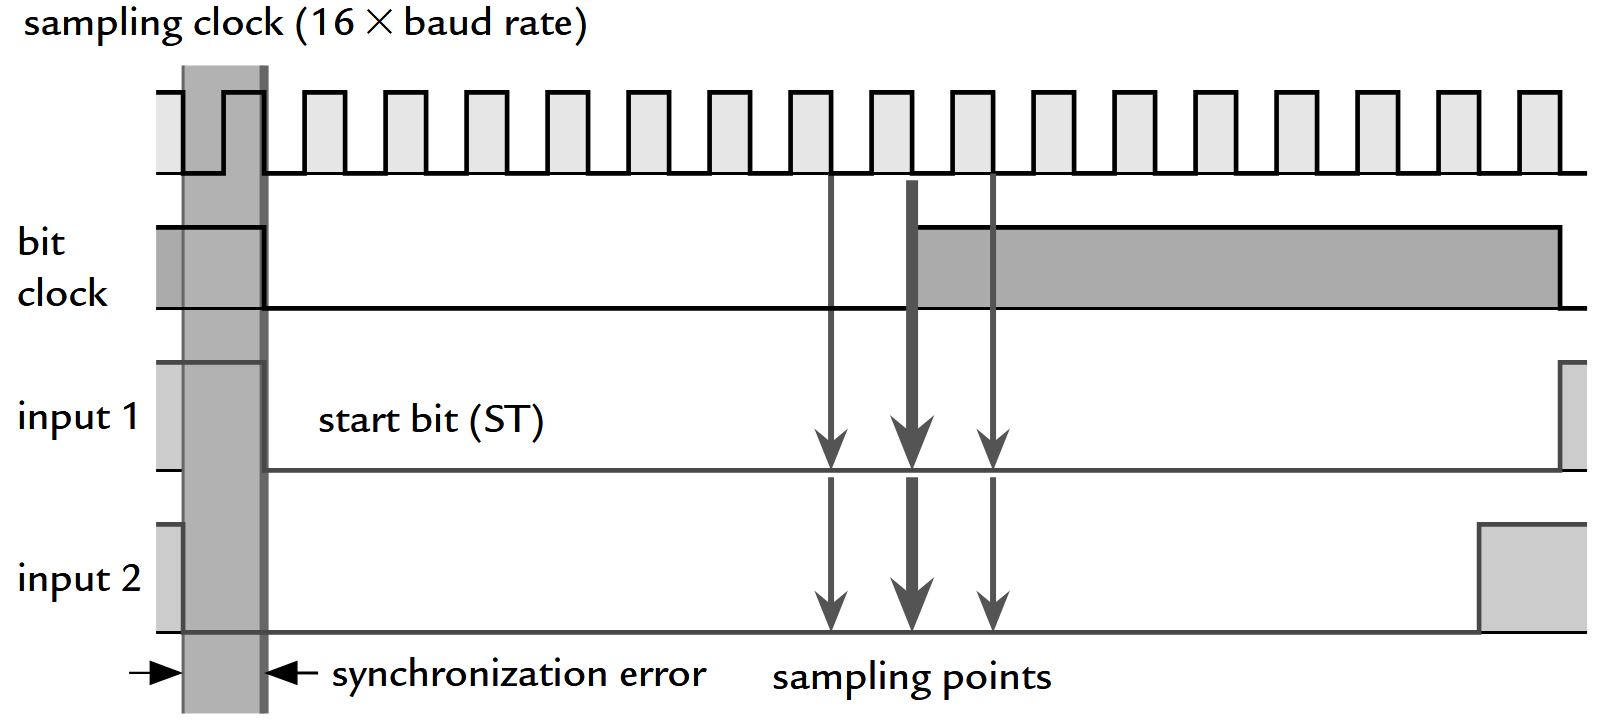
\includegraphics[width=1.0\textwidth]{../Bilder/uart_protocoll.png}
	\caption{UART \"ubertragung der Werte 0x55 und 0xFF\\\Zitat[S. 577, Abb. 10.19]{davies:msp430}}
	\label{fig:uart_uebertragung}
\end{figure}

Die interne Bit-Clock (\Abkuerzung{Bit-Clock}{BITCLK}) des Empf\"angers wird mit der fallenden Flanke des eingegangenen Start-Bits synchronisiert und operiert mit der Frequenz der eingestellten Baudrate. Da die fallende Flanke des Start-Bits zu einem beliebigen Zeitpunkt relativ zur Sampling Clock auftreten kann, entsteht ein initialer Synchronisationsfehler von bis zu einer halben Periode der Sampling Clock. Die in \Abbildung{uart_uebertragung} dargestellten Szenarien, bezeichnet als \glqq Input 1\grqq{} und \glqq Input 2\grqq{}, illustrieren die hieraus resultierende minimale und maximale zeitliche Verschiebung bei der Detektion der Startbit-Flanke, abh\"angig vom Phasenverh\"altnis zwischen dem Datensignal und der Sampling Clock. \Zitat[S. 476, kap. 18.2, S. 574, Kap. 10.12 \& S. 575, Kap. 10.12.1]{ti:slau272d, davies:msp430}

\subsubsection{Datenintegrit\"at, Fehlererkennung und weitere technischen Details}
\label{sec:datenintegritaet}

Zur Sicherstellung der Datenintegrit\"at kann eine Fehlererkennung, beispielsweise \"uber ein Parit\"atsbit, eingesetzt werden. Ein UART-Datenpaket, auch Frame genannt, besteht typischerweise aus einem Start-Bit, sieben oder acht Datenbits, einem optionalen Parit\"atsbit (f\"ur gerade oder ungerade Parit\"at) und mindestens einem Stop-Bit.

Die \"ubergeordnete Protokollebene implementiert \"ublicherweise komplexere Fehlererkennung oder -korrekturmechanismen, wie \zB Pr\"ufsummen (Checksum), die auf der UART-Kommunikation aufsetzt. Dar\"uber hinaus ist f\"ur eine erfolgreiche Kommunikation die eindeutige Festlegung der Bitreihenfolge essentiell. Die LSB-first-Konvention ist De-facto-Standard. \Zitat[S. 574, Kap. 10.12 \& S. 575, Kap. 10.12.1]{davies:msp430}

\newpage
Die automatische Fehlererkennung des Interfaces erm\"oglicht dem Benutzer eine schnelle Reaktion auf Grenzf\"alle und \"Ubertragungsfehler. \Tabelle{uart_error_flags} schl\"usselt alle wichtigen Fehler-Flags mit ihren zugeh\"origen Beschreibungen auf.

\begin{table}[h!]
	\small
	\centering
	\begin{tabular}{|l|c|p{8.5cm}|}
		\hline
		\textbf{Fehlerbedingung} & \textbf{Fehler-Flag} & \textbf{Beschreibung} \\
		\hline
		Framing-Fehler & UCFE & Tritt auf, wenn das Stoppbit nicht den erwarteten High-Pegel hat. Bei zwei Stoppbits werden beide gepr\"uft.\\\hline
		Parit\"atsfehler & UCPE & Entsteht durch eine Abweichung zwischen berechneter und tats\"achlicher Parit\"at. Adressbits werden in die Berechnung einbezogen.\\\hline
		Empfangs\"uberlauf & UCOE & Wenn ein neues Zeichen empfangen wird, bevor das vorherige gelesen wurde, wird ein \"Uberlauf erkannt.\\\hline
		Break-Bedingung & UCBRK & Wird erkannt, wenn alle Bits auf Low liegen (bei deaktivierter Baudratenerkennung). \Code{UCBRK} wird gesetzt und \ggf auch \Code{UCRXIFG}, wenn \Code{UCBRKIE} aktiv ist. \\\hline
	\end{tabular}
	\caption{UART-Fehlerbedingungen und zugeh\"orige Status-Flags des MSP430FR5729\\\Zitat[S. 483, Tab. 18-1]{ti:slau272d}}
	\label{tab:uart_error_flags}
\end{table}

Weitere technische Spezifikationen sind in \Tabelle{uart_features} zusammengefasst. Eine minimale Konfiguration der Schnittstelle auf den UART-Betrieb wird in \Kapitel{eUSCI_Konfiguration} detailliert beschrieben.

\begin{table}[h!]
	\small
	\centering
	\begin{tabular}{|p{6.5cm}|p{7.5cm}|}
		\hline
		\textbf{Funktion} & \textbf{Beschreibung} \\
		\hline
		Multiprozessor-Kommunikationsprotokolle & Unterst\"utzt integrierte Idle-Line- und Address-Bit-Protokolle f\"ur Kommunikation in Multiprozessorsystemen \\
		\hline
		Energiesparmodus-Unterst\"utzung & Startflankenerkennung im Empf\"anger erm\"oglicht automatisches Aufwachen aus LPMx-Modi (ausgenommen LPMx.5) \\
		\hline
		Fehlererkennung & Statusflags zur Detektion von Kommunikationsfehlern (z.\,B. Framing-, Parit\"ats- oder \"uberlauffehler) \\
		\hline
		Adresserkennung & Statusflags zur Erkennung von Datenpaketen in Multiprozessorsystemen \\
		\hline
		Interrupt-Unterst\"utzung & Unabh\"angige Interruptquellen f\"ur Empfang, \"Ubertragung, Startbit-Empfang sowie Abschluss der \"Ubertragung \\
		\hline
	\end{tabular}
	\caption{Technische Merkmale der UART-Schnittstelle des MSP430FR5729\\\Zitat[S. 476, kap. 18.2]{ti:slau272d}}
	\label{tab:uart_features}
\end{table}

\newpage
\subsubsection{Automatische Baudraten-Erkennung}
\label{sec:auto_baud}

Neben der festen Einstellung ermittelt die automatische Baudraten-Erkennung selbstst\"andig, \"uber eine \NeuerBegriff{Break/Sync Sequenz}, die vom Sender verwendete Baudrate. Diese Synchronisations-Sequenz besteht aus einem \NeuerBegriff{Break} und einem \NeuerBegriff{Sync} Feld. Der Bereich der erkennbaren Baudraten liegt im Oversampling-Modus zwischen 244 Baud (im niedrigfrequenz-Modus beginnend ab 15 Baud) und einem Megabaud. Ein Break umfasst 11 bis 21 \"ubertragen Nullen, w\"ahrend weitere Nullen einen \NeuerBegriff{Break Timeout}-Fehler ausl\"osen. Aus Konformit\"atsgr\"unden sollte das UART Protokoll auf acht Datenbits, mit LSB-first, keiner Parit\"at und einem Stop-Bit konfiguriert werden. In \Abbildung{auto_baud} ist die beschriebene Break/Sync-Sequenz dargestellt.

\newpage
\begin{figure}[h!]
	\centering
	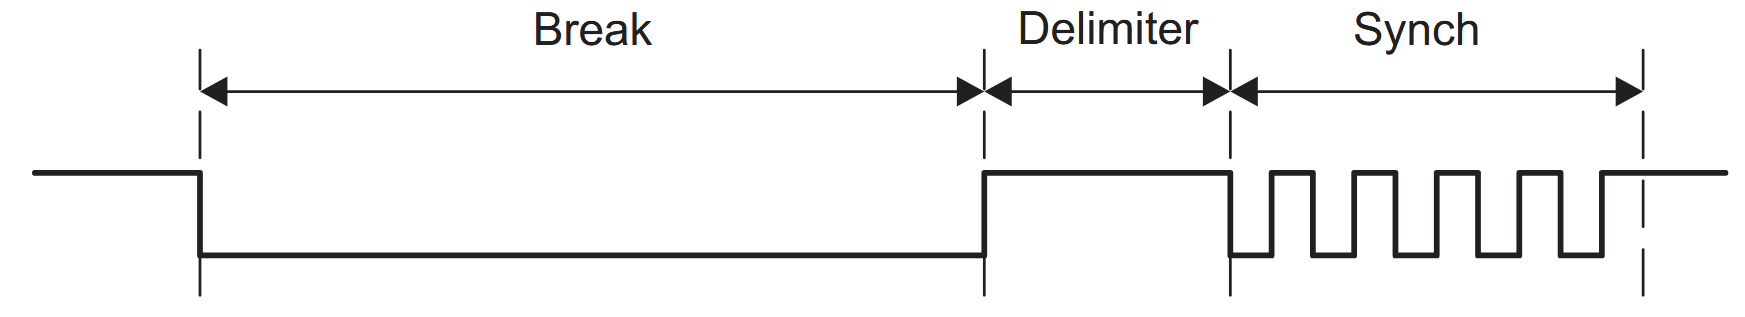
\includegraphics[width=1.0\textwidth]{../Bilder/auto_baud.png}
	\caption{Automatische Baudraten-Erkennung - Break/Sync Sequenz\\\Zitat[S. 481, Abb. 18-5]{ti:slau272d}}
	\label{fig:auto_baud}
\end{figure}

Der Synchronisations-Prozess beginnt mit der \"Ubertragung des hexadezimalen Wertes 0x55. Die Zeit zwischen der ersten und letzten fallenden Flanke wird gemessen, um die vom Sender verwendete Baudrate zu ermitteln. Dies ist grafisch in \Abbildung{sync_field} dargestellt. \"Uberschreitet die Messzeit den Maximalwert, tritt ein \NeuerBegriff{Sync-Timeout}-Fehler auf. Ist die Messung erfolgreich, liest das System nach dem Setzen des \NeuerBegriff{Receive Interrupt Flags} die Information aus. 

Nach jedem empfangenen Zeichen setzt das System das \Code{UCDORM}-Bit zur\"uck, da bei gesetztem Bit zwar alle Zeichen empfangen, aber nicht in das Puffer-Register der Schnittstelle geschrieben werden. \Zitat[S. 481, Kap. 18.3.4]{ti:slau272d}

\begin{figure}[h!]
	\centering
	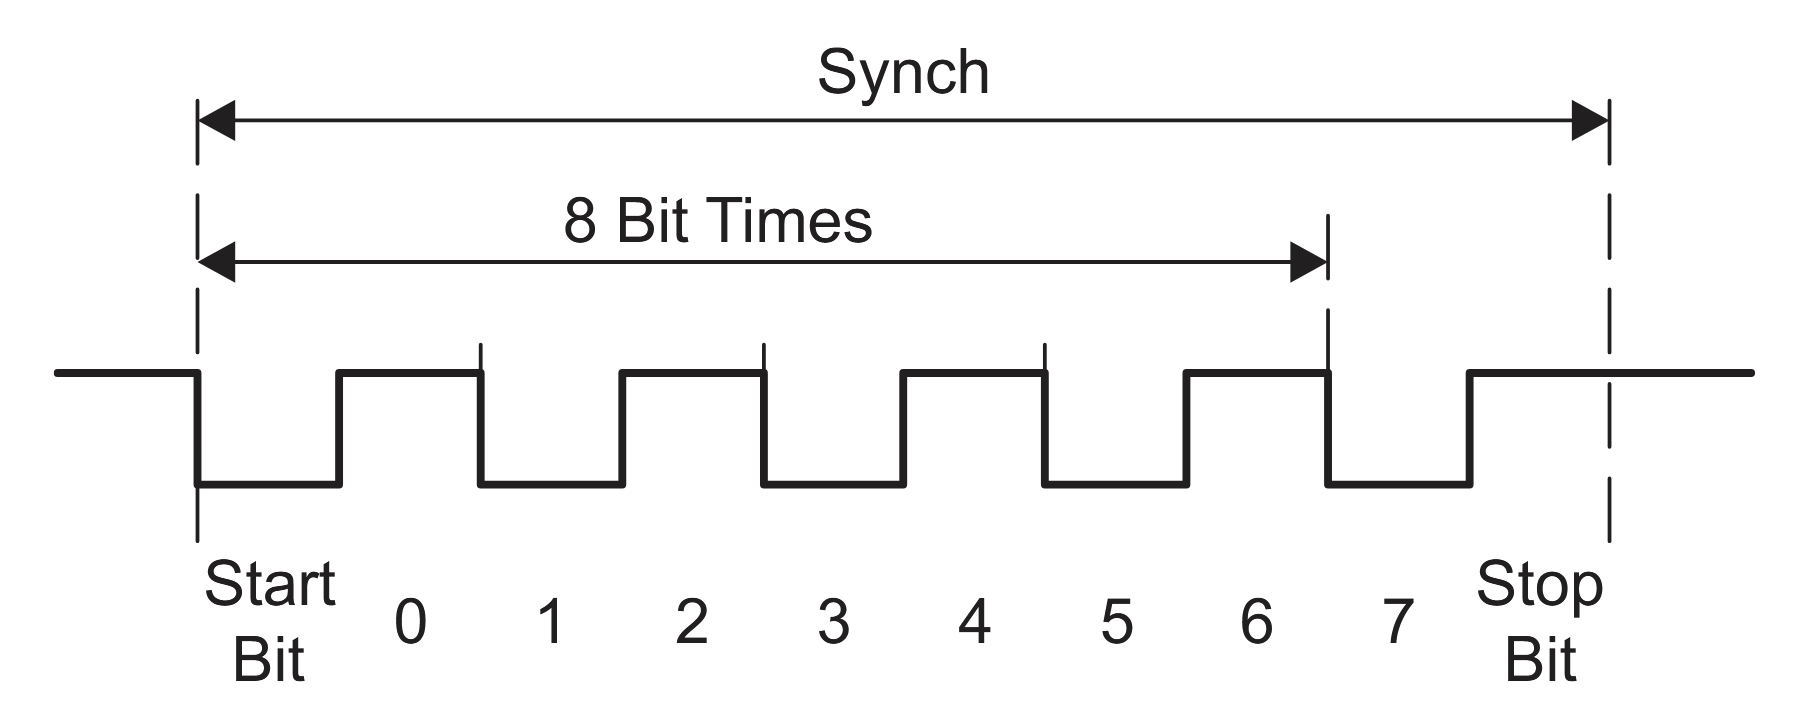
\includegraphics[width=0.95\textwidth]{../Bilder/sync_field.png}
	\caption{Automatische Baudraten-Erkennung - Sync Feld\\\Zitat[S. 481, Abb. 18-6]{ti:slau272d}}
	\label{fig:sync_field}
\end{figure}

\subsection{eUSCI-Konfiguration}
\label{sec:eUSCI_Konfiguration}

Die Initialisierung und Konfiguration des eUSCI\_A-Moduls f\"ur den UART-Betrieb folgt einer definierten Abfolge von Schritten zum Setzen von verschiedenen Bits und Werten in die daf\"ur vorgesehene Register. Der Prozess setzt das \Code{UCSWRST}-Bit zu Beginn. Dieses Bit erm\"oglicht die Konfiguration der Schnittstelle und schlie{\ss}t unerw\"unschtes Verhalten aus. Dabei wird das \Code{UCTXIFG}-Bit, zum freigeben der Konfiguration, gesetzt. Zudem werden diverse Interrupt-Enable-Bits wie \Code{UCRXIE} und \Code{UCTXIE} sowie Status- und Fehlerflags (\Code{UCRXIFG, UCRXERR, UCBRK, UCPE, UCOE, UCFE, UCSTOE, UCBTOE}) im \Code{UCAxSTATW}- und \Code{UCAxIFG}-Register gel\"oscht oder in einen definierten Anfangszustand gebracht. Dadurch gelangt das eUSCI\_A-Modul in einen sicheren Reset-Zustand. \Zitat[S. 478, Kap. 18.3.1]{ti:slau272d}

Nachdem das Modul sicher in den Reset-Zustand \"uberf\"uhrt wird, lassen sich weitere spezifische Konfigurationsparameter f\"ur den UART-Betrieb setzen. Hierzu z\"ahlen insbesondere die folgenden Kontrollbits im \Code{UCAxCTLWn}-Register, welche die grundlegenden Betriebscharakteristika des UART-Modus definieren, wie beispielsweise:

\begin{itemize}
	\item \textbf{UCPEN:} Aktiviert die Parit\"atspr\"ufung.
	\item \textbf{UCPAR:} Festlegen einer geraden oder ungeraden Parit\"at.
	\item \textbf{UCMSB:} Legt die Bitreihenfolge fest (LSB- oder MSB-first).
	\item \textbf{UC7BIT:} Konfiguriert die Datenl\"ange auf 7 oder 8 Bit.
	\item \textbf{UCSPB:} Anzahl der Stop-Bits.
	\item \textbf{UCMODEx:} W\"ahlt den UART-Modus. (\zB 0 f\"ur Normal-Betrieb, 3 f\"ur  automatische Baudratenerkennung)
	\item \textbf{UCSYNC:} F\"ur den asynchronen UART-Betrieb muss dieses Bit auf 0 gesetzt werden.
	\item \textbf{UCSSELx:} Taktquelle f\"ur Baudratengenerator.
\end{itemize}

\"Uber die genannten grundlegenden Einstellungen hinaus existieren weitere spezifischere Kontrollbits. Beispielsweise ist das \Code{UCRXEIE}-Bit zur freigabe des Fehler-Interrupts und das \Code{UCBRKIE} zum aktivieren der Break-Interrupts zust\"andig. 

\newpage
Spezialfunktionen wie der Multiprozessor-Modus, welcher \"uber das \Code{UCTXADDR}-Bit gesteuert wird, oder das Senden eines Break-Zeichens mittels \Code{UCTXBRK} sind f\"ur eine Standard-UART-Konfiguration oft zu vernachl\"assigen, sofern diese Funktionalit\"aten nicht explizit gefordert sind. \Zitat[S. 495, Kap. 18.4.1 \& S. 496, Kap. 18.4.2]{ti:slau272d}

Eine weitere essenzielle Konfiguration f\"ur den UART-Betrieb ist die der Baudrate. Diese erfolgt \"uber das \Code{UCAxBRW}-Register und das \Code{UCAxMCTLW}-Register. Die korrekte Wertermittlung f\"ur diese Register ist direkt von der Frequenz der zuvor mittels \Code{UCSSELx} gew\"ahlten Taktquelle sowie der angestrebten Baudrate abh\"angig. Der \glqq Family User's Guide\grqq{} des MSP430FR5729 von Texas Intruments liefert f\"ur die Berechnung dieser Werte detaillierte Formeln und Beispieltabellen. Das \Code{UCAxBRW}-Register nimmt den ganzzahligen Anteil des Baudratenteilers (Prescaler) auf. Das \Code{UCAxMCTLW}-Register beinhaltet die Konfiguration f\"ur die Modulation der Frequenz, sowie das Bit zur Aktivierung des Oversampling-Modus. Durch das \Code{UCBRFx}-Bit wird, in der ersten Modulationsstufe, die Feineinstellung des Prescalers vorgenommen. In der zweiten Modulationsstufe wird durch \Code{UCBRSx} ein Modulationsmuster f\"ur die BITCLK festgelegt. Im letzten Bitfeld kann nun der Oversampling-Modus aktiviert oder deaktiviert werden. \Zitat[S. 487, Kap. 18.3.10 \& S. 497, Kap. 18.4.3, 18.4.4]{ti:slau272d}

Obwohl weitere spezifische Einstellungen m\"oglich sind, w\"urde deren detaillierte Er\"orterung den Rahmen dieser \"Ubersicht \"uberschreiten. Eine unerl\"assliche, abschlie{\ss}ende Konfigurationsma{\ss}nahme vor der Inbetriebnahme betrifft jedoch die Port-Pins: Die f\"ur den UART Betrieb verwendeten Pins m\"ussen, \"uber die Function-Select-Register (\Code{PxSEL}), auf die asynchrone UART-Kommunikation konfiguriert werden. \Zitat[S. 294, Kap. 8.2.5]{ti:slau272d}

Nach Abschluss aller Konfigurationseinstellungen wird das \Code{UCSWRST}-Bit im \Code{UCAxCTLW0}-Register gel\"oscht (auf \grq{}0\grq{} zur\"uckgesetzt). Dieser Schritt hebt den Reset-Zustand auf und aktiviert das eUSCI-Modul mit der zuvor definierten Konfiguration. Optional k\"onnen nun die gew\"unschten Interrupts, wie \zB der Sende- (\Code{UCTXIE}), Empfangs- (\Code{UCRXIE}), Transmit-Complete- (\Code{UCTXCPTIE}) oder Start-Bit-Interrupt (\Code{UCSTTIE}), im \Code{UCAxIE}-Register aktiviert werden, um eine ereignisgesteuerte Datenverarbeitung zu erm\"oglichen. \Zitat[S. 502, Kap. 18.4.10]{ti:slau272d}

Diese sorgf\"altige Konfigurationssequenz ist entscheidend f\"ur die zuverl\"assige Funktion der UART-Schnittstelle des MSP430-Mikrocontrollers.

\newpage
\subsection{Zusammenfassung}
\label{sec:eUSCI_Zusammenfassung}

Die vorangegangenen Kapitel haben die Kommunikationsschnittstelle des MSP430FR5729 im UART-Betrieb detailliert beleuchtet. Das eUSCI-Modul dient der serielle Kommunikation mit Peripherieger\"aten oder anderen Systemen. Dazu werden synchrone Protokolle wie SPI und I$^{2}$C und asynchrone Protokolle wie UART bereitgestellt.

Im Rahmen dieser Arbeit zeigte sich (siehe \Kapitel{Einordnung_Schnittstellen}), dass das asynchrone Kommunikationsprotokoll UART am besten f\"ur die Kommunikation zwischen dem MSP430FR5729 und einem PC-System geeignet ist. Die Bewertung der Schnittstellen erfolgte unter den Gesichtspunkten Implementierungsaufwand, Robustheit, Interruptf\"ahigkeit und Kompatibilit\"at.

Wesentliche Aspekte des UART-Betriebs ist die asynchrone Natur der Kommunikation und die wechselseitige Daten\"ubertragung zwischen zwei Parteien mittels Baudraten-Synchronisation, auch Vollduplex-Kommunikation genannt. Wichtige Merkmale hierzu ist das Datenformat (\zB acht Datenbits, LSB-first, ein SP) und die Mechanismen zur Fehlererkennung (\zB Framing-, Parity-, Overrun-Error).

Die automatische Baudraten-Erkennung erh\"oht bei der Verkn\"upfung mehrerer Kommunikationspartner \"uber dieselbe Leitung die Flexibilit\"at, steigert jedoch auch die Komplexit\"at. Da f\"ur die aktuelle Anwendung keine Verbindung mit unterschiedlichen Baudraten \"uber eine einzelne Schnittstelle erforderlich ist, wird diese Funktion nicht ben\"otigt.

Die zentralen Schritte zur Konfiguration des eUSCI-Moduls f\"ur den UART-Betrieb umfasst das Einleiten des eUSCI-Software-Resets, das Setzen und gegebenenfalls R\"ucksetzen notwendiger Steuerbits in den Kontrollregistern, die Feinabstimmung der gew\"unschten Baudrate \"uber Prescaler-Werte und schlie{\ss}lich das Aufheben des Reset-Zustandes zur Aktivierung des Moduls.

\Abbildung{BlockDiagramm_eUSCI_A_UART} zeigt ein detailliertes Blockdiagramm des eUSCI\_A-Moduls in der konfigurierten UART-Betriebsart.

\newpage
\begin{figure}[h!]
	\centering
	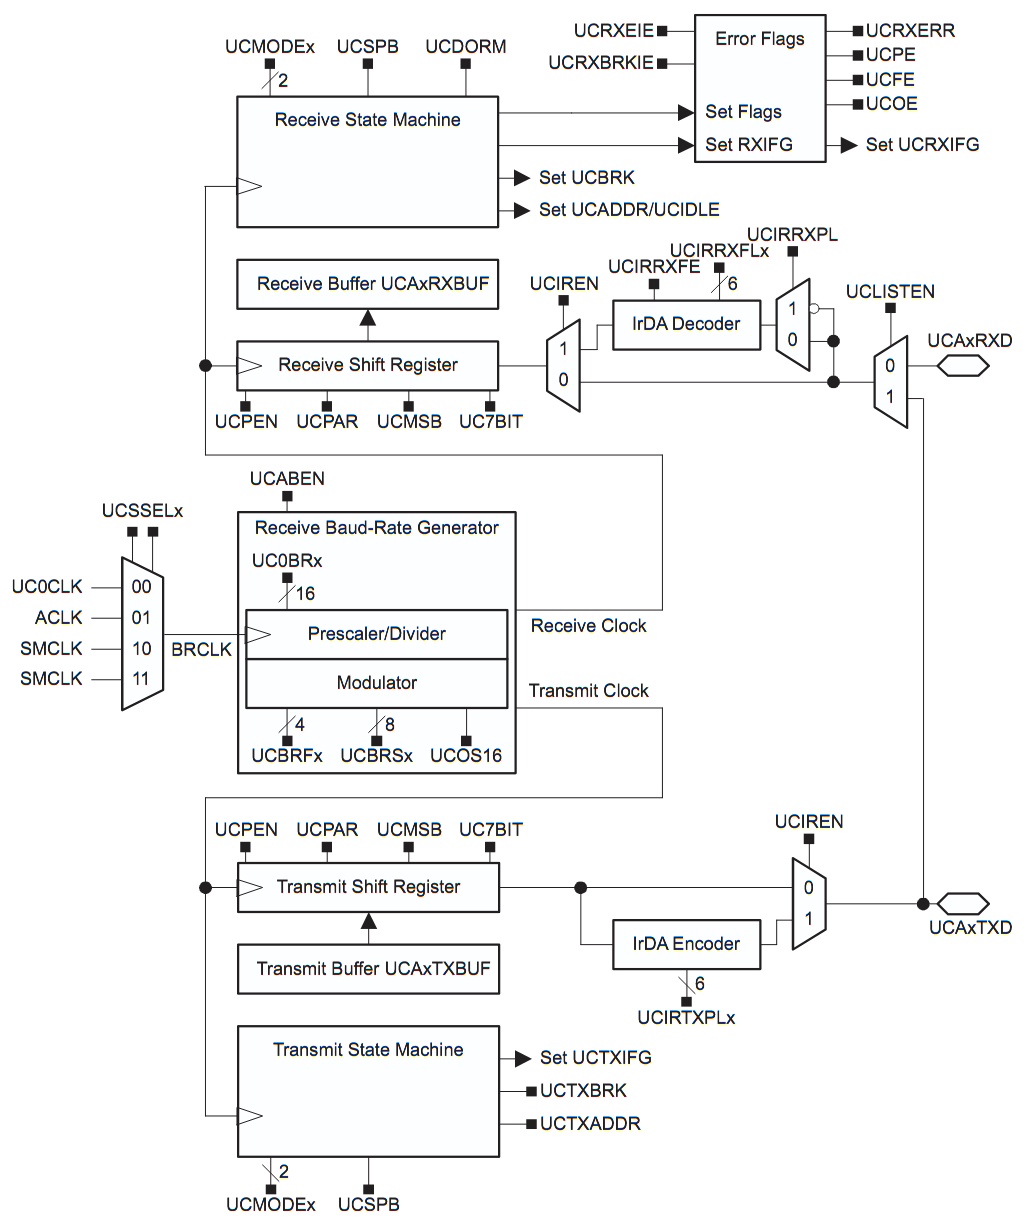
\includegraphics[width=1.0\textwidth]{../Bilder/eUSCI_UART.png}
	\caption{eUSCI Typ A -- UART-Modus\\\Zitat[S. 477, Kap. 18.2]{ti:slau272d}}
	\label{fig:BlockDiagramm_eUSCI_A_UART}
\end{figure}

% !TEX encoding = UTF-8 Unicode
% !TEX root =  ../Bachelorarbeit.tex

\chapter{Entwicklung}

Aufbauend auf den in den vorangegangenen Kapiteln -- \ref{TIMER&ISR} und \ref{eUSCI} -- vermittelten theoretischen Grundlagen zu Timern, Interrupt Service Routinen (ISR) und dem Enhanced Universal Serial Communication Interface des Mikrocontrollers MSP430FR5729, widmet sich dieses Kapitel der Entwicklung und praktischen Umsetzung der interruptgesteuerten Benutzerschnittstelle.

Zun\"achst erfolgt die systematische Konzeptionierung des \glqq Observer-Moduls\grqq. Dieses dient als zentrale Instanz zur Erfassung und Bearbeitung von Befehlseingaben sowie zur Steuerung zugeh\"origer Systemausgaben. Dieses Modul stellt somit die Grundlage f\"ur die Interaktion zwischen Benutzer und Mikrocontroller dar.

Im weiteren Verlauf wird die Konfiguration der interruptgesteuerten Kommunikation \"uber die UART-Schnittstelle erarbeitet. Hierbei liegt der Fokus auf zuverl\"assigkeit und robustheit sowie deren sicherer Ausgabe unter Echtzeitbedingungen.

Abschlie{\ss}end werden zentrale Debugging-Mechanismen vorgestellt, evaluiert und exemplarisch in Form von softwarebasierten Breakpoints implementiert. Ziel ist es, die Robustheit, Echtzeitf\"ahigkeit sowie den funktionalen Umfang der zu entwickelnden Komponente zu validieren und zu evaluieren.

Die Integration von Breakpoints erm\"oglicht es, gezielt in den Programmablauf eingreifen zu k\"onnen, ohne den Systemzustand zu beeintr\"achtigen. Insbesondere zu integrierende Funktionen f\"ur das lesen und beschreiben von Speicherzellen profitieren hiervon. Wird ein Breakpoint erreicht, k\"onnen diese Befehle kontrolliert und st\"orungsfrei ausgef\"uhrt werden, da das Hauptprogramm w\"ahrenddessen in einen definierten Haltemodus versetzt wird. Auf diese Weise l\"asst sich eine konsistente Speicherzugriffslogik realisieren, die auch w\"ahrend kritischer Zust\"ande wie Kontextwechsel zuverl\"assig funktioniert.\AI

\section{Konzeprionierung Observer-Modul}
\label{ObserverModulKonzept}

Die zentrale Einheit zur Verarbeitung eingehender Befehle und zur Steuerung s\"amtlicher Funktionen stellt das Observer-Modul dar. Es vereint die Interrupt-Basierte Abarbeitung sowie das Senden von Daten und Empfang externer Steuerbefehle. Die in den Kapiteln \ref{TIMER&ISR} und \ref{eUSCI} erl\"auterten Technologien des MSP430FR5729 bilden hierzu die technische Grundlage.

Solange kein Befehl \"uber die Eingabetaste eines verbundenen PCs best\"atigt wurde, verbleibt das Modul im Ruhezustand. Bereits ab dem ersten \Fachbegriff{Zeichenkombination aus Buchstaben (lateinisches Alphabet) und Ziffern (0–9)}{alphanumerischen}[alphanumerisch] Zeichen wird ein \glqq Time-Out\grqq-Timer aktiviert. Erfolgt keine abschlie{\ss}ende Eingabe innerhalb eines definierten Zeitintervalls, wird diese zur\"uckgesetzt und ein \glqq Time-Out-Error\grqq generiert. Mit erfolgreicher Best\"atigung wird der Timer deaktiviert und die Befehlsinterpretation eingeleitet. Das Ergebnis der Befehlsverarbeitung wird \"uber UART zur\"uckgegeben. Etwaige Fehler im Ablauf werden mithilfe eines Fehlervektors priorisiert, gespeichert und entsprechend ausgegeben. Das Observer-Modul arbeitet statusorientiert und verarbeitet Ereignisse gem\"a{\ss} ihres Auftretens. \Abbildung{StateMachine_ObserverModul} zeigt einen voll Umfassenden \Fachbegriff{Auch endlicher Automat, ist ein mathematisches Modell zur Beschreibung von Systemen mit endlich vielen Zust\"anden, das \"Uberg\"ange zwischen diesen in Abh\"angigkeit von Eingaben definiert; \Vgl Hopcroft, J.E., Motwani, R., Ullman, J.D. (2006): Introduction to Automata Theory, Languages, and Computation.}{Zustandsautomaten}.

\begin{figure}[h!]
	\centering
	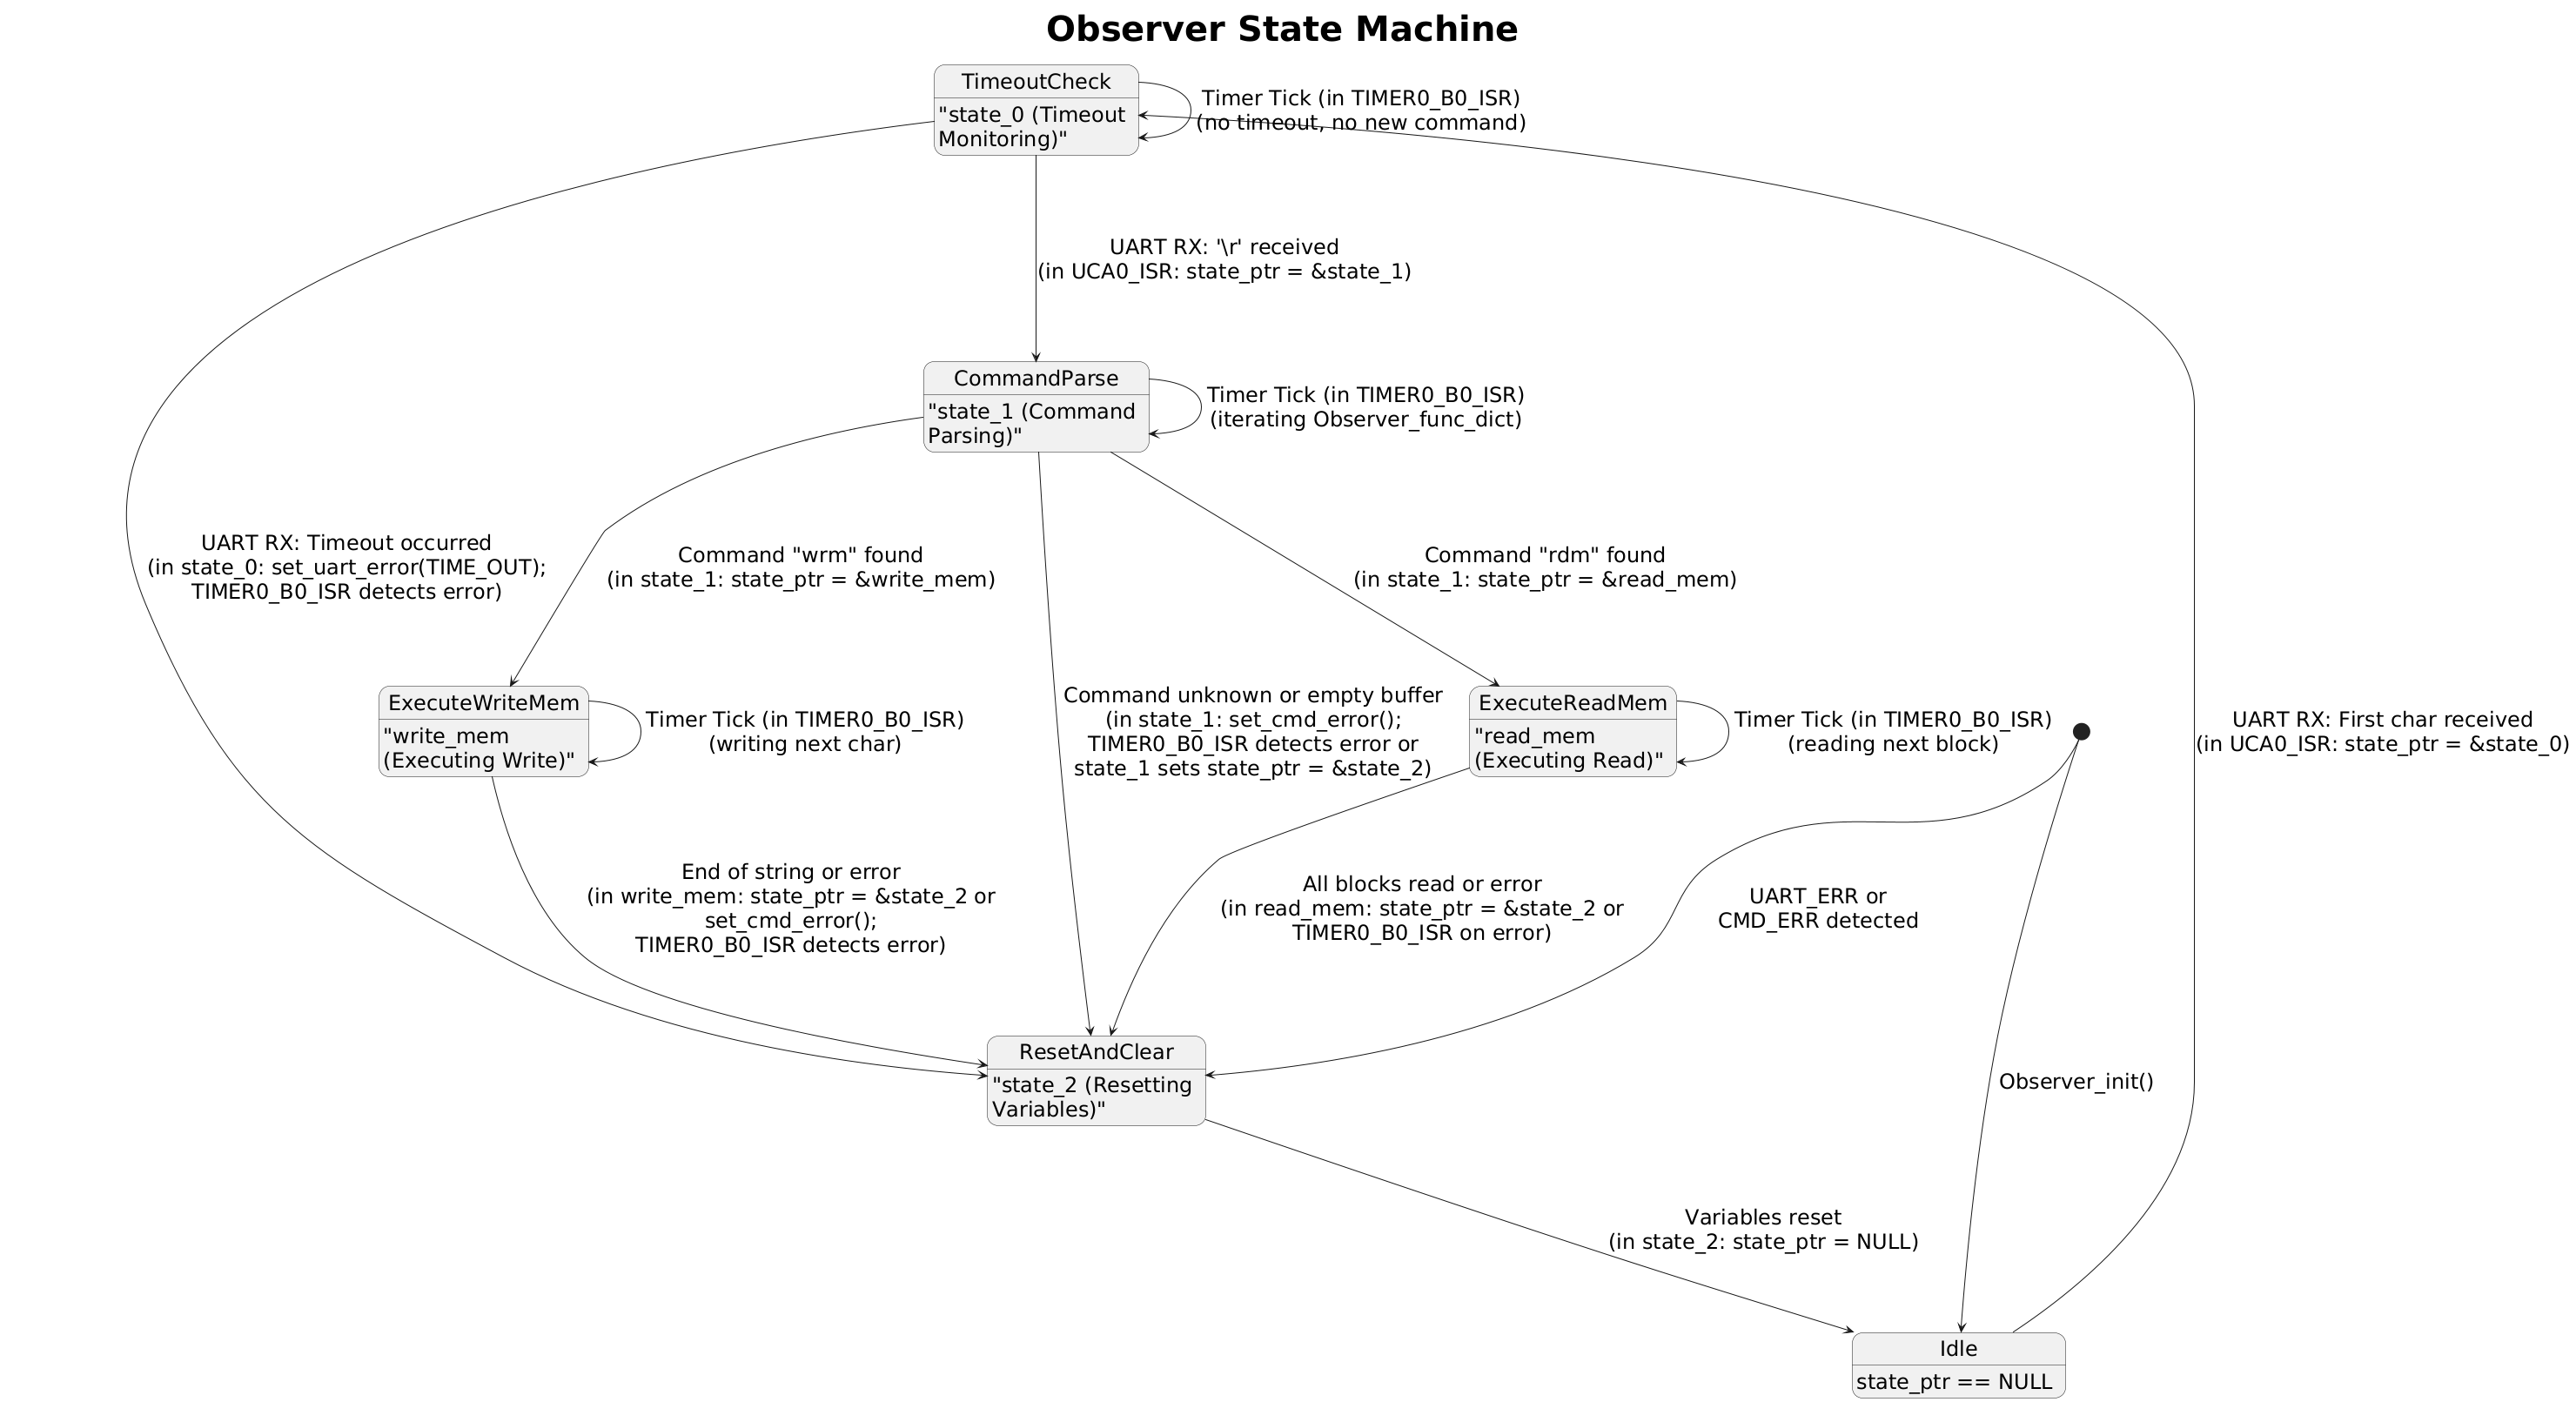
\includegraphics[width=1.0\textwidth]{../Bilder/observer_state_machine.png}
	\caption{Zustandsautomat -- Observer-Modul}
	\label{fig:StateMachine_ObserverModul}
\end{figure}

Ein funktionales Modul, welches die daf\"ur ben\"otigten Hardware-Komponenten – insbesondere Interrupt Service Routines (ISR) und das eUSCI-Modul – integriert, erfordert eine \"offentlich zug\"angliche Initialisierungsmethode, die von der Hauptroutine aufgerufen wird. Diese Methode \"ubernimmt die Konfiguration der Steuerregister sowie die Initialisierung ben\"otigter Variablen und Datenstrukturen.

F\"ur die Ein- und Ausgabe \"uber UART kann die in \ref{eUSCI_Konfiguration} beschriebene Konfiguration \"ubernommen werden. Folgende Einstellungen haben sich dabei als vorteilhaft erwiesen:

\begin{itemize}
	\item Gerade Parit\"at
	\item LSB-first
	\item Acht-Datenbits
	\item Ein Stoppbit
	\item UART-Modus
	\item Asynchroner Modus
	\item ACLK-Taktquelle
	\item Aktiver Fehler-Interrupt
	\item Aktiver Break-Interrupt
	\item 9600 Baud
	\item 16-faches Oversampling
	\item Entprellzeit von rund 100ns
\end{itemize}

Die Verarbeitung von Ereignissen wie Befehlsinterpretation, Fehlerausgabe und Eingabe-Time-Out wird \"uber eine gemeinsame ISR realisiert. Eine daf\"ur passende Periodendauer betr\"agt 10\,ms. Kapitel \ref{TIMER&ISR} beschreibt die verf\"ugbaren Timer des MSP430FR5729. Aufgrund der in diesem Zusammenhang dargestellten Eigenschaften erweist sich ein Timer vom Typ B als besonders geeignet, da seine erweiterte Konfiguration -- gegen\"uber des Timers von Typ A -- eine skalierbare und anpassungsf\"ahige Implementierung des Moduls im Hinblick auf zuk\"unftige Systemanforderungen erlaubt. Neben den funktionalen Vorteilen ergibt sich die Wahl des Timers auch deshalb, weil im System bereits s\"amtliche Timer vom Typ A anderweitig genutzt werden.

\newpage
Die relevante Konfiguration der Capture-/Compare-Register basiert auf folgenden Parametern:

\begin{itemize}
	\item Compare-Modus
	\item UP-Modus
	\item ACKL als Taktquelle
	\item Input Teiler jeweils auf acht
	\item Compare-Register auf 96 setzen
	\item Aktivierter Timer-Interrupt
\end{itemize}

Der Wert f\"ur das Compare-Register ergibt sich aus folgender Formel:

\[
\text{Compare-Wert} = \frac{f_\text{ACLK} \cdot T_\text{Periode}}{\text{Teiler}_1 \cdot \text{Teiler}_2} = \frac{614{,}4\,\text{kHz} \cdot 10\,\text{ms}}{8 \cdot 8} = 96
\]

Weitere Initialisierungen umfassen:
\begin{itemize}
	\item Puffervariablen zur Zeichenspeicherung,
	\item Event- und Fehlerflags,
	\item Laufvariablen und Zeiger zur schnellen Navigation innerhalb von Eingabepuffern,
	\item sowie Funktionszeiger f\"ur die Ereignisverarbeitung.
\end{itemize}

Ein besonderer Vorteil ergibt sich durch den Einsatz eines \Fachbegriff{Datenstruktur, die Schl\"ussel-Wert-Paare speichert und schnellen Zugriff auf Werte \"uber ihre eindeutigen Schl\"ussel erlaubt.}{Dictionarys}[Dictionary], das Befehlen eindeutig Funktionszeiger zuordnet.

\newpage
Alle beschriebenen Komponenten und ihre funktionale Zuordnung sind in \Abbildung{UmlDiagram_ObserverModul} zusammengefasst.

\begin{figure}[h!]
	\centering
	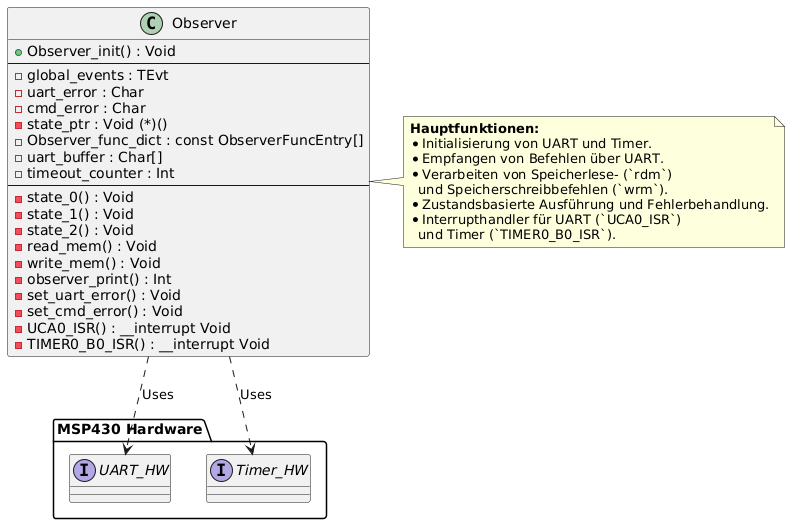
\includegraphics[width=1.0\textwidth]{../Bilder/observer_class_diagram.png}
	\caption{UML-Diagram -- Observer-Modul}
	\label{fig:UmlDiagram_ObserverModul}
\end{figure}

Ausgehend vom grundlegenden Architekturkonzept des Observer-Moduls erfolgt im Folgenden die detaillierte Implementierung der Funktionen f\"ur das interruptgesteuerte Lesen und Schreiben \"uber die serielle Schnittstelle.\AI


\newpage
\section{Interruptgesteuertes Lesen und Schreiben}
\label{Interruptgesteuertes_Lesen&Schreiben}


\newpage
\section{Debugging-Methoden: Hardware- vs. Software-Breakpoints}
\label{Hardware_VS_Software_Breakpoints}

Im Kontext der Fehlersuche und Programmanalyse in Embedded Systems stellen \Fachbegriff{Bezeichnet in der Softwareentwicklung eine vom Entwickler bewusst gesetzte Unterbrechung im Programmablauf, die typischerweise zur Laufzeit-Debugging-Zwecken verwendet wird. Beim Erreichen dieses Punkts wird die Ausf\"uhrung des Programms angehalten, sodass der aktuelle Zustand (\zB Variableninhalte, Stack, Speicher) analysiert werden kann.}{Breakpoints}[Breakpoint] ein fundamentales Werkzeug dar. Sie erm\"oglichen es, die Ausf\"uhrung eines Programms an einer vordefinierten Stelle zu unterbrechen, um den internen Zustand des Systems zu inspizieren. Grunds\"atzlich lassen sich zwei prim\"are Arten von Breakpoints unterscheiden: Software-Breakpoints und Hardware-Breakpoints, deren Implementierung und Eigenschaften sich signifikant unterscheiden.

Software-Breakpoints werden zur aktiven Laufzeit des Programms durch einen direkten Eingriff in den ausf\"uhrbaren Code im Speicher des Mikrocontrollers realisiert. An der Zieladresse wird hierbei die urspr\"ungliche Programminstruktion tempor\"ar durch eine Breakpoint-Instruktion oder einen Trap-Befehl ersetzt, der einen Software-Interrupt oder eine Exception ausl\"ost. Sobald der Programmz\"ahler diese modifizierte Stelle erreicht, unterbricht der Mikrocontroller den normalen Programmfluss der Programmz\"ahler stoppt und eine Debug-Routine wird ausgef\"uhrt. Der \Fachbegriff{Ein Werkzeug zur schrittweisen Ausf\"uhrung und Analyse von Programmen. Es erlaubt das Setzen von Haltepunkten, das \"uberpr\"ufen von Speicherinhalten und das Nachvollziehen von Kontrollfl\"ussen zur Fehlersuche und -behebung.}{Debugger} kann diesen Zustand erkennen, die urspr\"ungliche Instruktion wiederherstellen und dem Entwickler die Kontrolle \"ubergeben. Durch diesen Mechanismus sind Software-Breakpoints hochflexibel und k\"onnen an nahezu jeder beliebigen Stelle im beschreibbaren Code-Speicher (wie RAM oder FRAM) gesetzt werden.

Die Vorteile des softwarebasierten Ansatzes liegen prim\"ar in der M\"oglichkeit, eine praktisch unbegrenzte Anzahl von Breakpoints im System zu verwenden, sowie in den geringen Anforderungen an zus\"atzliche, dedizierte Hardwarekomponenten auf dem Zielsystem selbst. Die grundlegende F\"ahigkeit, Interrupts oder Exceptions zu behandeln, ist hierf\"ur ausreichend. \Zitat[Kap. 4.7.16]{ti:CCS}

Gegen\"uber den Software-Breakpoints bieten hardwarebasierte Breakpoints den Vorteil, dass sie Programmunterbrechungen auch in solchen Speichersegmenten erm\"oglichen, die schreibgesch\"utzt sind (z.B. ROM oder spezifisch gesch\"utzte Flash-Bereiche). Ein weiterer entscheidender Vorteil ist ihre Nicht-Intrusivit\"at: Da keine Modifikation des Programmcodes stattfindet, werden weder die Konsistenz des Codes im Speicher noch das pr\"azise Echtzeitverhalten (Timing) des Programms durch den Breakpoint-Mechanismus selbst beeinflusst. \Zitat[Kap. 4.7.16]{ti:CCS}, \Zitat[S. 54, Kap. 4.3]{ti:spru296}

Um dies jedoch zu erreichen, ben\"otigen Hardware-Breakpoints ein dediziertes Hardwaremodul innerhalb des Mikrocontrollers. Im Falle der MSP430-Mikrocontrollerfamilie ist dies das \NeuerBegriff{Embedded Emulation Module (EEM)} \Zitat[S. 569, Kap. 21]{ti:slau272d}. Dieses Modul beinhaltet spezielle Hardwareregister, typischerweise Adresskomparatoren, welche die Speicheradresse des Befehls halten, an welcher bei \"ubereinstimmung mit dem Programmz\"ahler ein Breakpoint ausgel\"ost werden soll. Da der Breakpoint durch externe Hardwarelogik ausgel\"ost wird und nicht durch eine im Programmablauf ausgef\"uhrte Instruktion, m\"ussen seitens des Breakpoint-Mechanismus selbst keine Registerinhalte oder Stack-Elemente explizit zwischengespeichert und im Nachhinein wiederhergestellt werden. Ganz im Unterschied wie es bei einem durch einen Software-Breakpoint induzierten Interrupt der Fall sein kann. Die Zustandssicherung erfolgt erst durch die Debug-Routine nach erfolgter Unterbrechung. Der wesentliche Nachteil hierbei ist allerdings die strikte Limitierung der Anzahl gleichzeitig setzbarer Hardware-Breakpoints, welche direkt von der Anzahl der im EEM verf\"ugbaren Komparator-Register abh\"angt. F\"ur den MSP430 sind dies oft nur zwei oder drei \Zitat[vgl. Kap. 7.1]{ti:CCS}.

Diese Gegen\"uberstellung offenbart einen klaren \Fachbegriff{Abw\"agung zwischen zwei konkurrierenden Zielen, Konzepten, oder \"ahnlichem, bei der die Verbesserung des einen mit der Verschlechterung des anderen einhergeht.}{Trade-off}: Hardware-Breakpoints gl\"anzen durch ihre Transparenz und die F\"ahigkeit, in gesch\"utzten Speicherbereichen zu operieren, sind jedoch eine knappe Ressource. Software-Breakpoints hingegen bieten eine hohe Flexibilit\"at und nahezu unbegrenzte Verf\"ugbarkeit, gehen aber mit einer leichten Modifikation des Programmcodes und potenziellen, wenn auch meist minimalen, Timing-Ver\"anderungen einher. Angesichts der begrenzten Anzahl an Hardware-Breakpoints auf der MSP430-Plattform, die insbesondere bei komplexeren Debugging-Szenarien schnell ersch\"opft sein k\"onnen, erweist sich die Implementierung von Software-Breakpoints als eine pragmatische und oft notwendige Erweiterung der Debugging-M\"oglichkeiten. Um die technischen Rahmenbedingungen f\"ur die Realisierung solcher Software-Breakpoints auf dem MSP430FR5729 sowie die Interaktion mit der Debugging-Infrastruktur genauer zu verstehen, ist eine detaillierte Betrachtung des eingesetzten Debug-Adapters und seiner Funktionsweise unerl\"asslich. 

Dar\"uber hinaus existiert auch noch eine spezielle Art von Breakpoints welcher von einem Speicherzugriff ausgl\"o{\ss}t wird. Watchpoints k\"onnen Grenzf\"alle identifizieren um dadurch invalide Speicheradressen und zugriffe sowie Puffer\"uberl\"aufe zu analysieren. \Zitat[Kap. 7.4.16.2]{ti:CCS}

Die nachfolgende Analyse des MSP-FET Debuggers wird weitere Aspekte des Software und Hardware-Basierten Debuggings beleuchten und die Grundlage f\"ur die sp\"atere Implementierungsstrategie legen.\AI

\subsection{Der MSP-FET Download Adapter im Detail}
\label{sec:MSP-FET_Debugger}

Die effektive Nutzung von sowohl Hardware- als auch Software-Breakpoints auf dem MSP430FR5729 ist ma{\ss}geblich von der externen Debugging-Hardware und -Software abh\"angig. Als zentrale Schnittstelle zwischen der Entwicklungsumgebung auf dem Host-PC und dem Ziel-Mikrocontroller dient in diesem \"okosystem der \textbf{\Abkuerzung{Flash Emulation Tool}{MSP-FET} (Flash Emulation Tool) Debugger}. Dieses externe Ger\"at, zu sehen in \Abbildung{msp_fet}, stellt die physische und logische Verbindung zum MSP430 her und erm\"oglicht tiefgreifende Eingriffe und Beobachtungen w\"ahrend der Programmausf\"uhrung.

\begin{figure}[h!]
	\centering
	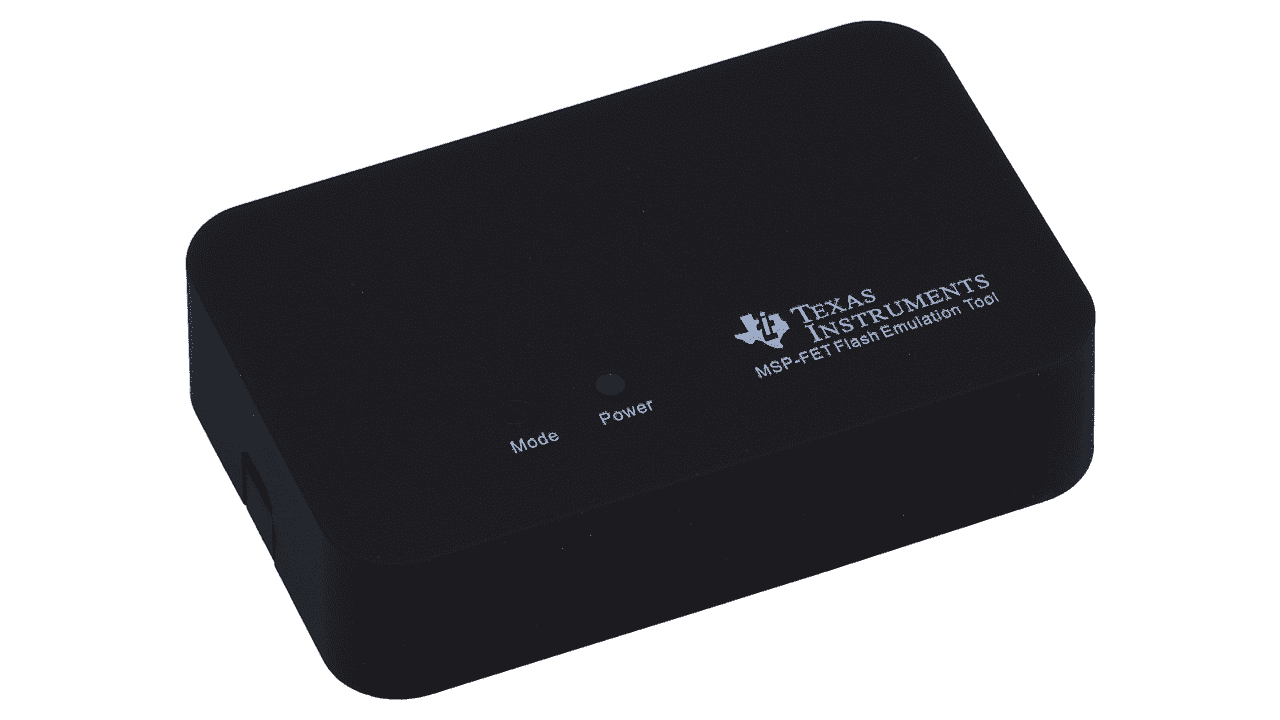
\includegraphics[width=1.0\textwidth]{../Bilder/msp_fet.png}
	\caption{Flash Emulation Tool Programmer and Debugger \Zitat{ti:MSP_FET}}
	\label{fig:msp_fet}
\end{figure}

Der MSP-FET kommuniziert mit dem MSP430-Mikrocontroller typischerweise \"uber standardisierte (Debug-)Schnittstellen wie \textbf{\Abkuerzung{Joint Test Action Group}{JTAG} (Joint Test Action Group)} oder das von Texas Instruments entwickelte \Fachbegriff{Zweidraht-Variante des JTAG-Protokolls, die Pin-Anzahl am Target reduziert und besonders f\"ur platzkritische Anwendungen von Vorteil ist.}{Spy-Bi-Wire}. (\Abkuerzung{Spy-Bi-Wire}{SBW}) \"uber diese Schnittstellen erh\"alt der MSP-FET Zugriff auf das EEM des MSP430FR5729. Wie im vorherigen Abschnitt \ref{Hardware_VS_Software_Breakpoints} dargelegt, ist das EEM f\"ur die Realisierung von Hardware-Breakpoints zust\"andig. Der MSP-FET agiert hierbei als Vermittler, der die vom Entwickler in der \NeuerBegriff{IDE (Integrated Development Environment)} gesetzten Hardware-Breakpoint-Adressen in die entsprechenden Register des EEM schreibt und die vom EEM generierten Haltesignale empf\"angt und an die IDE weiterleitet. Somit ist der MSP-FET unerl\"asslich f\"ur die Konfiguration und Nutzung der limitierten, aber pr\"azisen Hardware-Breakpoint-Ressourcen des Mikrocontrollers. \Zitat[S. 58, Kap. 3.4]{davies:msp430}

Dar\"uber hinaus spielt der MSP-FET eine ebenso gro{\ss}e Rolle f\"ur die Implementierung und Handhabung von Software-Breakpoints. Die F\"ahigkeit, den Speicher des MSP430FR5729 (sowohl RAM als auch das beschreibbare FRAM) zur Laufzeit zu lesen und zu schreiben, ist die Grundvoraussetzung, um Instruktionen mit einer Software-Breakpoint-Routine zu ersetzen. Der Debugger liest \"uber den MSP-FET die urspr\"ungliche Instruktion an der Zieladresse aus, ersetzt diese durch eine Breakpoint-Instruktion und, nach dem Ausl\"osen des Software-Interrupts, stellt er die urspr\"ungliche Instruktion wieder her. Ferner erm\"oglicht der MSP-FET die Steuerung des Programmflusses (Anhalten, Starten, Einzelschrittbetrieb) und den Zugriff auf CPU-Register und Speicherinhalte, was f\"ur die Analyse des Systemzustands an einem Breakpoint unerl\"asslich ist. Das vom Software-Breakpoint ausgel\"oste Interrupt- oder Exception-Signal wird ebenfalls \"uber die Debug-Schnittstelle an den MSP-FET und somit an die Host-Debugger-Software gemeldet. Wie solche Hardware und Software-Breakpoints in der Entwicklungsumgebung aussehen, ist in \Abbildung{CCS_SetBR} zu sehen. Das \glqq H/W\grqq oder \glqq S/W\grqq innerhalb der eckigen Klammern steht wahlweise f\"ur \glqq Hardware\grqq oder \glqq Software\grqq welches von einem \glqq BP\grqq f\"ur \glqq Breakpoint\grqq erg\"anzt wird.

\begin{figure}[h!]
	\centering
	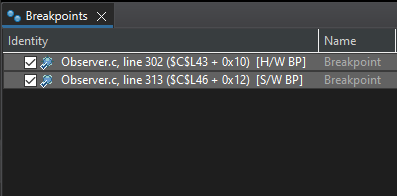
\includegraphics[width=0.75\textwidth]{../Bilder/HW_SW_Breakpoint.png}
	\caption{Code Composer Studio - Breakpoint \"Ubersicht}
	\label{fig:CCS_SetBR}
\end{figure}

Es ist wichtig zu verstehen, dass der MSP-FET prim\"ar die Kommunikationsinfrastruktur und die Low-Level-Zugriffsmechanismen bereitstellt. W\"ahrend er das Setzen von Hardware-Breakpoints direkt \"uber das EEM steuert, stellt er f\"ur Software-Breakpoints die notwendigen Lese-, Schreib- und Kontrolloperationen zur Verf\"ugung. Die eigentliche Logik eines Software-Breakpoints – das hei{\ss}t, welche Instruktion als Breakpoint-Befehl dient, wie die urspr\"ungliche Instruktion gesichert und wiederhergestellt wird sowie der resultierende Trap behandelt wird – muss in der Debugger-Software auf dem Host und gegebenenfalls durch eine minimale Debug-Monitor-Routine auf dem Target implementiert werden, wobei der MSP-FET als Br\"ucke dient. \Zitat[S. 56, Kap. 10]{ti:slau157as, ti:slau654e}

Die Kenntnis der Funktionalit\"aten und der Arbeitsweise des MSP-FET ist somit entscheidend f\"ur die Entwicklung einer robusten Software-Breakpoint-L\"osung. Er definiert die Grenzen und M\"oglichkeiten, wie mit dem Target-System interagiert werden kann, um Breakpoints zu setzen, Zustandsinformationen abzufragen und die Programmausf\"uhrung zu steuern. Die im Folgenden zu entwickelnde Strategie zur Implementierung von Software-Breakpoints muss sich daher eng an den durch den MSP-FET und die Debug-Schnittstelle des MSP430FR5729 gegebenen Rahmenbedingungen orientieren.

\newpage
\subsection{Konzeptionierung von Software-Breakpoints}
\label{sec:KonzeptionierungSoftwareBreakpoints}

Zur Realisierung von Breakpoints existieren mehrere Ans\"atze. Ein bew\"ahrter Einstieg besteht darin, etablierte Debugger und ihre Architektur zu studieren. Im Embedded‑ und Low‑Power‑Bereich kommen beispielsweise Werkzeuge wie \NeuerBegriff{TRACE32}, \NeuerBegriff{M-Core} oder das \NeuerBegriff{MSP-FET} von Texas Instruments zum Einsatz. Diese Debugger setzen Hardware-Breakpoints \"uber spezielle Debug‑Interfaces um und bieten damit eine hohe Zuverl\"assigkeit bei minimaler Eingriffstiefe in das Laufzeitsystem.

Im Gegensatz dazu zielt die hier vorgestellte L\"osung auf eine Abwandlung der Software-Breakpoints ab, die direkt den Programmspeicher manipuliert. Dabei wird, in dieser Implementierung, an der gew\"unschten Halteadresse der originale Maschinenbefehl durch einen Sprungbefehl (Jump) ersetzt, der auf eine speziell implementierte \NeuerBegriff{Breakpoint-Handler}-Routine verweist. Beim Erreichen dieses Befehls wird zun\"achst ein kritischer Abschnitt eingeleitet: Es werden die f\"ur den Prozess relevanten Register (R1 bis R3) – namentlich \Fachbegriff{Ein Register, das die Speicheradresse des derzeitigen Befehls enth\"alt.}{Program Counter} (\Abkuerzung{Program Counter}{PC}), \Fachbegriff{Ein Register, das die Speicheradresse des letzten oder ersten Datenelements im Stack speichert.}{Stack Pointer} (\Abkuerzung{Stack Pointer}{SP}), \Fachbegriff{Register f\"ur eine Reihe von Flags, die von der arithmetisch-logischen Einheit in Abh\"angigkeit der zuletzt durchgef\"uhrten Rechenoperation gesetzt werden.}{Statusregister} (\Abkuerzung{Status Register}{SR}) und \ggf mehrere \NeuerBegriff{General-Purpose-Register (R4 bis R15)} – gesichert und Interrupts deaktiviert, um eine atomare Kontextsicherung zu gew\"ahrleisten \Zitat[S.91, Kap. 4.3]{ti:slau272d}. Anschlie{\ss}end erfolgt der \"ubergang in die Handler-Routine, die das gesamte System bis auf das Observer-Modul blockiert und so das Auslesen und Manipulieren von Speicherinhalten erm\"oglicht.

Nach der Analyse kann der urspr\"ungliche Programmzustand durch das laden der Registers\"atze wiederhergestellt werden. Eine explizite reaktivierung der Interrupts ist daher nicht n\"otig. Der Compiler stellt hierf\"ur \Fachbegriff{Compiler-spezifische, vordefinierte Funktionen, die direkt in optimierten Assemblercode umgesetzt werden.}{Compiler-Intrinsics}[Compiler-Intrinsic] bereit wie \Code{\_\_get\_SR()}, \Code{\_\_get\_SP()} und \Code{\_\_set\_interrupt\_state()} \Zitat[S.137, Kap. 6.8.1]{ti:slau132r}. Auf diese Weise wird ein vollst\"andiger Zyklus von Unterbrechung, Inspektion und Fortsetzung des Programmflusses realisiert, ohne dass das Hauptprogramm von dem Observer-Modul tiefgreifender beeinflusst wird.

Vor diesem Hintergrund wird in den folgenden Abschnitten die Konzeptionierung erweiterter Software-Breakpoints im Detail erl\"autert und auf die daf\"ur notwendigen Voraussetzungen eingegangen.

\subsubsection{Verwendung eines Sprungbefehls anstelle einer Trap}
\label{sec:JumpVsTrap}

Wie in Abschnitt \ref{Hardware_VS_Software_Breakpoints} erl\"autert, basieren klassische software-Breakpoints h\"aufig auf sogenannten Trap-Instruktionen. Das Debugging-Framework der Entwicklungsumgebung unterst\"utzt dies unter anderem \"uber die \NeuerBegriff{General Extension Language} (\Abkuerzung{General Extension Language}{GEL}) – ein Makro- und Skriptsystem, das die Initialisierung von Systemen sowie die Steuerung von Debug-Sitzungen erm\"oglicht. Dar\"uber hinaus erlaubt GEL auch das Setzen von Breakpoints, Speicherzugriffe und die Ablaufkontrolle des Programms \Zitat[Kap. 7.7, 7.7.8.6 \& 7.7.8.7]{ti:CCS}.

F\"ur diese Arbeit war es jedoch erforderlich, dass bei Ausl\"osen eines Breakpoints benutzerdefinierte Routinen aus dem Observer-Modul aktiv bleiben und verwendet werden k\"onnen (\Vgl Abschnitt \ref{Interruptgesteuertes_Lesen&Schreiben}). Diese Funktionalit\"aten sind mit dem Standardverhalten von GEL-Traps nicht kompatibel, da sie typischerweise nur auf Debugger-seitige Prozesse abzielen und keine Kontextintegration benutzerdefinierter Routinen auf dem Zielsystem erlauben.

Aus diesem Grund wurde bewusst auf die Verwendung eines Trap-Mechanismus verzichtet und stattdessen ein direkter Sprungbefehl (Jump) auf eine benutzerdefinierte Breakpoint-Handler-Routine implementiert. Dadurch wird sichergestellt, dass das Observer-Modul auch w\"ahrend einer Unterbrechung aktiv bleibt und die Kontrolle \"uber Register- und Speicherzugriffe erhalten bleibt.

\subsubsection{Implementierung erweiterter Software Breakpoints}
\label{sec:ImplementierungSoftwareBreakpoints}

Die Grundidee von Software-Breakpoints besteht darin, an einer Stelle im Programmspeicher, an der ein g\"ultiger Maschinenbefehl (\Fachbegriff{Auch op code oder operation code, ist eine meist in hexadezimaler Schreibweise angegebene Zahl, die die Nummer eines Maschinenbefehls f\"ur einen bestimmten Prozessortyp angibt.}{Opcode}) liegt, diesen tempor\"ar durch einen Sprung auf die Breakpoint-Handler-Routine zu ersetzen. Zun\"achst wird der originale Opcode gesichert, um ihn sp\"ater unver\"andert wieder einsetzen zu k\"onnen. Die Auswahl der Adresse erfordert, dass diese auf ein g\"ultiges Befehlswort ausgerichtet ist und im Stack-Bereich liegt, um Kollisionen auf das Code-Segmenten zu vermeiden. Zudem muss die Interpretation der Adresse und des zu schreibenden Sprungbefehls den aktiven Adressierungsmodus ber\"ucksichtigen.

Die Implementierung gliedert sich in folgende Schritte:
\begin{enumerate}
	\item \textbf{Adressvalidierung:} Pr\"ufen, ob die Zieladresse auf vier Byte ausgerichtet ist und im Stack liegt.
	  
	\item \textbf{Kontext-Sicherung:} In einem kritischen Abschnitt werden PC, SP, SR und alle modifizierten Register in einem Puffer abgelegt. Hierbei ist zu beachten, dass die Breite des PC vom Adressierungsmodus abh\"angt, worauf entsprechend r\"ucksicht genommen werden muss. \Zitat[S. 97, Kap. 4.4]{ti:slau272d}
	
	\item \textbf{Ersetzen des Opcodes:} Der Original-Opcode (vier Byte) wird durch den vier-Byte-Sprungbefehl (zwei Byte f\"ur den Instruction-Code, zwei Byte f\"ur die Zieladresse der Handler-Routine) \"uberschrieben. \Zitat[S.161, Kap. 4.6.2.28]{ti:slau272d}
	
	\item \textbf{Ausf\"uhrung des Breakpoint-Handlers:} Beim Eintreten des Breakpoint-Opcodes springt der PC in die Handler-Routine, die das System an weiterer Ausf\"uhrung hindert und stattdessen das Observer-Modul f\"ur weitere Debug-Schritte aktiv h\"alt.
	
	\item \textbf{Kontext-Wiederherstellung:} Nach Abschluss der Debug-Aktion werden alle Register und der urspr\"ungliche Opcode wiederhergestellt, bevor der normale Programmablauf fortgesetzt wird.
\end{enumerate}

Diese Vorgehensweise stellt die R\"uckkehr zum urspr\"unglichen Systemzustand – einschlie{\ss}lich des Originalen-Opcodes – sicher und garantiert die Konsistenz des Programms.

Um die im vorigen Abschnitt \ref{sec:KonzeptionierungSoftwareBreakpoints} skizzierten Konzepte robust umzusetzen, sind die im n\"achsten Abschnitt, technischen Details wie Instruktionsl\"angen und Speicher-Alignment, zu betrachten.\AI

\subsubsection{Instruktionsl\"angen, Speicher-Alignment und Adress-Modi}
\label{sec:TechnischeUmsetzunSoftwareBreakpoints}

Die Manipulation von Befehlen im Stack ist hoch kritisch, da das Hauptprogramm keine Kenntnis vom Observer-Modul hat und eine falsche Adressierung, unterschiedlichen Adressierungs-Modi oder unvollst\"andige Opcode-substituierung zu undefiniertem Verhalten f\"uhren kann. Drei zentrale Aspekte sind dabei zu beachten:

\begin{itemize}
	\item \textbf{Speicher-Alignment:} MSP430-Instruktionen sind grunds\"atzlich an geraden Speicheradressen ausgerichtet. Vor jedem Schreib- oder Lesezugriff muss daher sichergestellt werden, dass die Zieladresse eine gerade Adresse ist. Zugriffe auf ungerade Adressen k\"onnen zu undefiniertem Verhalten f\"uhren, sofern keine Fehlerbehandlung erfolgt. Dar\"uber hinaus sind Adressen, die in der Mitte eines Opcodes liegen, ung\"ultig und d\"urfen nicht als Breakpoint oder adressiert werden.
	
	\item \textbf{Opcode-L\"angen:} W\"ahrend einzelne Maschinenbefehle in der Regel zwei bis vier Bytes belegen, k\"onnen komplexe Instruktionen – etwa \Code{CMP.B} – bis zu sechs Bytes lang sein, wie in \Abbildung{DisassemblyOpcodeLaengen} zu sehen. \Zitat[S.165, Kap. 4.6.2.32]{ti:slau272d} Diese Variabilit\"at erschwert das gezielte \"Uberschreiben von genau vier Byte, die f\"ur die Jump-Instruktion einschlie{\ss}lich Zieladresse ben\"otigt werden. Unter diesen Randbedingungen besteht die Gefahr, dass entweder zu viele oder zu wenige Bytes \"uberschrieben werden, was zu ung\"ultigen oder unbeabsichtigten Instruktionen f\"uhren kann.
	
	\item \textbf{Adressierungs Modus:} Der Speicher, im Umfang von einem Megabyte, kann \"uber sieben unterschiedliche arten Adressiert werden. Wahlweise kommen 16 oder 20-Bit Adressen zum Einsatz. Diese Variabilit\"at der Adressierungsmodi und die damit einhergehenden unterschiedlichen Adressbreiten haben tiefgreifende Konsequenzen.\Zitat[S. 97, Kap. 4.4]{ti:slau272d}
\end{itemize}

\begin{figure}[h!]
	\centering
	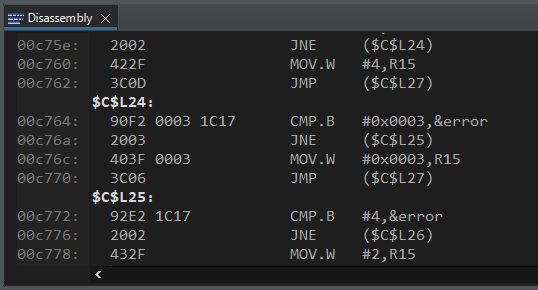
\includegraphics[width=0.75\textwidth]{../Bilder/OpcodeLaengen.png}
	\caption{Code Composer Disassembly Modus - Opcode l\"angen}
	\label{fig:DisassemblyOpcodeLaengen}
\end{figure}

Das Sichern und Wiederherstellen von Registern und des Originalen Opcodes reicht daher nicht aus, insbesondere angesichts den variablen Instruktionsl\"angen und komplexer Adressierungsmodi. 

Die gr\"o{\ss}e der Opcodes h\"angt von folgenden Parametern ab. Die Grundlegende l\"ange einer Instruktion des MSP430 liegt bei zwei Byte. Darin ist die Operation, wie beispielsweise \Code{MOV.W}, sowie die Register- und Adressierungsart kodiert. Unterschiedliche Adressierungen von Operanden \"uber Adressierungsmodi wie \glqq \Fachbegriff{Operand ist direkt in der Instruktion enthalten – also ein fester Wert, nicht aus dem Speicher.}{Immediate}\grqq , \glqq \Fachbegriff{Operand befindet sich an einer feste Speicheradresse.}{Absolute} \grqq oder \glqq \Fachbegriff{Operand ist nicht direkt gegeben, sondern steht an der Adresse, die ein Register enth\"alt.}{Indirect}\grqq, haben zur Folge, dass die Adressen oder Konstanten zus\"atzlich als \Fachbegriff{Synonym f\"ur 2 Byte gro{\ss}e Datenbreite}{Word} (2 Byte) oder \Fachbegriff{Synonym f\"ur 4 Byte gro{\ss}e Datenbreite}{extended Word} (4 Byte) kodiert werden. \Zitat[S. 97, Kap. 4.4]{ti:slau272d}

Ein Beispiel hierzu, woraus sich der 6-Byte lange Opcode, zum Vergleichen des Speicherinhalts des Registers \glqq \&error\grqq  mit dem Hexadezimalen Wert \glqq 0x0003\grqq, aus \Abbildung{DisassemblyOpcodeLaengen} zusammensetzt:
\\\textbf{\Code{CMP.B \#0x0003, \&error}}
\begin{itemize}
	\item \textbf{1 Byte} Opcode f\"ur \Code{CMP.B}
	\item \textbf{1 Byte} Modus f\"ur Quell-Operand und Ziel-Operand (Immediate -> Absolute)
	\item \textbf{2 Byte} Immediate-Wert f\"ur Konstante \glqq 0x0003\grqq
	\item \textbf{2 Byte} Absolute-Adresse f\"ur Label \glqq \&error\grqq
\end{itemize}
\Zitat[S. 147, Kap. 4.6.2.14 \& S. 112, Kap. 4.4.7 \& S. 108, Kap. 4.4.4]{ti:slau272d}

Diese Analyse verdeutlicht die komplexit\"at der Manipulation und Wiederherstellung von Instruktionen im Stack. Eine Kopie des Stacks schafft dabei eine sichere Umgebung, in welcher der bestehende Opcode Manipuliert wird. Hierbei muss die Kopie die unterschiedlichen Adressformate und die potenziell im Stack gespeicherten, modusabh\"angigen Zeiger korrekt abbilden oder transformieren. Dies garantiert ein sicheres zur\"uckkehren in die Hauptroutinen, sowie eine Robuste Ausf\"uhrung der Funktion zum verarbeiten der \ggf mehreren Breakpoints.

Dies erschwert die Umsetzung und erh\"oht die Komplexit\"at der Routine erheblich, wodurch Timing und Konsistenz gef\"ahrdet werden. Im anschlie{\ss}enden Fazit werden die gewonnenen Erkenntnisse bewertet, offene Fragestellungen skizziert und ein Ausblick auf weiterf\"uhrende Arbeiten gegeben.

\subsection{Fazit zur Umsetzung von Software Breakpoints}
\label{sec:FazitSoftwareBreakpoints}

Die Realisierung von Software-Breakpoints auf dem Low‑Power‑Mikrocontroller MSP430FR5729 erfordert ein tiefgehendes Verst\"andnis der Prozessor‑Architektur, der Instruktionsformate, der vielf\"altigen Adressierungs-Modi und ihrer Auswirkungen auf die Speicherverwaltung und der nebenl\"aufigen Abl\"aufe im System. Die Analyse der Problemstellung hat ergeben, dass unter anderem kritische Bereiche atomar bearbeitet, Register und Stack-Zust\"ande zuverl\"assig gesichert und Intrinsics korrekt eingesetzt werden m\"ussen. Zudem sind umfangreiche Funktionen zur \"uberwachung und Protokollierung des Systemzustands zu implementieren.

Die erwartete komplexit\"at inklusive der Anforderungen an Robustheit, Echtzeitf\"ahigkeit und m\"oglichst geringem Eingriff in den Betrieb \"uberschreitet den Rahmen einer \"ublichen Bachelorarbeit. Eine vollst\"andige, ausgereifte Implementierung w\"are mit dem Umfang einer Masterarbeit oder vergleichbarer Forschungsarbeiten m\"oglich. Dennoch bildet dieses Thema eine exzellente Grundlage f\"ur weiterf\"uhrende Arbeiten in den Bereichen eingebettete Echtzeitsysteme und Debugging‑Technologien, insbesondere in Bezug auf Architekturen mit flexiblen, aber komplexen Speicheradressierungsmechanismen.



% !TEX encoding = UTF-8 Unicode
% !TEX root =  ../Bachelorarbeit.tex
\chapter{Fazit und kritische Bewertung}
\label{cha:Fazit}


\section{Das Ergebnis}
\label{sec:Ergebnis}

\section{Die Bewertung der Frameworks Extbase und Fluid}
\label{sec:BewertungFrameworks}

\section{Ein Ausblick}
\label{sec:EinAusblick}








\clearpage{}
\pagenumbering{Roman}
\setcounter{page}{7} %%% Dieser Pagecounter muss entsprechend der verbrauchten Seiten im Inhaltsverzeichnis angepasst werden. Endet das IHV bei Seite III, so muss hier 4 eingetragen werden


% Literaturverzeichnis ---------------------------------------------------------------------------------
%   Das Literaturverzeichnis wird aus der BibTeX-Datenbank "Bibliographie.bib"
%   erstellt.
% ------------------------------------------------------------------------------------------------------
\bibliography{Bibliographie} % Aufruf: bibtex Masterarbeit
\bibliographystyle{natdin} % DIN-Stil des Literaturverzeichnisses


% Restliche Verzeichnisse ------------------------------------------------------------------------------
\listoffigures{} % Abbildungsverzeichnis
\listoftables{} % Tabellenverzeichnis
\renewcommand{\lstlistlistingname}{Verzeichnis der Listings}
\lstlistoflistings{} % Listings-Verzeichnis


% Index ------------------------------------------------------------------------------------------------
%   Zum Erstellen eines Index, die folgende Zeile auskommentieren.
% ------------------------------------------------------------------------------------------------------
%\printindex


% Selbständigkeitserklärung ----------------------------------------------------------------------------
% !TEX encoding = UTF-8 Unicode
% !TEX root =  Bachelorarbeit.tex

\addchap{Eidesstattliche Versicherung}
Ich, \autor, Matrikel-Nr.\ \matrikelnr, versichere hiermit, dass ich meine \art\xspace mit dem Thema
\begin{quote}
\textit{\titel} \textit{\untertitel}
\end{quote}
selbständig verfasst und keine anderen als die angegebenen Quellen und Hilfsmittel benutzt habe, wobei ich alle wörtlichen und sinngemäßen Zitate als solche gekennzeichnet habe. Die Arbeit wurde bisher keiner anderen Prüfungsbehörde vorgelegt und auch nicht veröffentlicht.

Mir ist bekannt, dass ich meine \art\xspace zusammen mit dieser Erklärung fristgemäß nach Vergabe des Themas in dreifacher Ausfertigung und gebunden im Prüfungsamt der \hochschule\xspace abzugeben oder spätestens mit dem Poststempel des Tages, an dem die Frist abläuft, zu senden habe.\\[6ex]

\ort, den \today


\rule[-0.2cm]{5cm}{0.5pt}

\textsc{\autor} 
 


% Anhang -----------------------------------------------------------------------------------------------
%   Die Inhalte des Anhangs werden analog zu den Kapiteln inkludiert.
%   Dies geschieht in der Datei "Anhang.tex".
% ------------------------------------------------------------------------------------------------------
\begin{appendix}
    \clearpage{}
    \pagenumbering{roman}
    \chapter{Anhang}
    \label{sec:Anhang}
    % Rand der Aufzählungen in Tabellen anpassen
    \setdefaultleftmargin{1em}{}{}{}{}{}
    % !TEX encoding = UTF-8 Unicode
% !TEX root =  Bachelorarbeit.tex

\section{Verwendete Hilfsmittel}

\subsection{Erkl\"arung zur Nutzung von KI-Sprachmodellen zur stilistischen \"Uberarbeitung}
Im Rahmen dieser Bachelorarbeit wurden \NeuerBegriff{Large Language Models}, namentlich ChatGPT-4o und GeminiAI 2.5 Flash, zur kritischen Bewertung und konstruktiven \"Uberarbeitung der sprachlichen Ausdrucksweise eingesetzt. Dies umfasst stilistische und Grammatikalische Optimierung in folgenden Bereichen:

\begin{itemize}
	\item Verbesserung der Lesbarkeit und sprachlichen Klarheit,
	\item Vereinheitlichung des wissenschaftlichen Ausdrucks,
	\item Korrekturvorschl\"age von Grammatik-, Rechtschreibung- und Zeichensetzung.
\end{itemize}

Alle Kapitel, die \"uberarbeitet werden, sind am Ende mit einem Hinweis in einer Fu{\ss}note gekennzeichnet.

Die inhaltliche Verantwortung f\"ur alle Aussagen, Argumentationen und wissenschaftlichen Schlussfolgerungen liegt vollst\"andig bei dem Autor. Die genannten KI-Modelle werden \textbf{nicht} zur Generierung fachlicher Inhalte, zur Datenanalyse oder zur Strukturierung argumentativer Abschnitte verwendet.

Die Verwendung dieser Werkzeuge erfolgt unter Beachtung geltender ethischer Richtlinien f\"ur wissenschaftliche Arbeiten sowie der Anforderung an Eigenst\"andigkeit und Transparenz.

\newpage
\subsection{Erkl\"arung zur Erstellung von Diagrammen}

Zur Erstellung von Diagrammen wird das Tool \textit{PlantUML} (verf\"ugbar unter \url{https://www.plantuml.com}) verwendet. 

Mit Hilfe des Tools werden verschiedene UML-Diagramme wie Aktivit\"atsdiagramme, Klassendiagramme und Zustandsdiagramme (State-Machine-Diagramme) modelliert. PlantUML erm\"oglicht die textuelle Beschreibung von Diagrammen, welche anschlie{\ss}end automatisch als grafische Darstellung generiert werden. Dies erleichtert sowohl die Versionierung als auch die Nachvollziehbarkeit der Diagrammerstellung im Entwicklungsprozess.
\end{appendix}

\end{document}
